\documentclass[twoside]{book}
\usepackage{html}	% html.sty (from latex2html) is in this directory
\usepackage{epsfig}
\usepackage{wrapfig}
\usepackage{fancybox}
\usepackage{latexsym}
\usepackage{makeidx}
\usepackage{xspace}
\usepackage{verbatim}
\makeindex

% These commands are based on the fancybox package.  Use \keycap{X} to print
% a glyph resembling a keyboard `X' key.  Use \button{Y} to print a reasonable
% facsimile of an Open Look button labelled `Y'.  Use \menubutton{Z} to print
% a similar Open Look menu button labelled `Z'.  Use \amenubutton{X} to print
% an abbreviated menu button labelled `X'.
\setlength{\fboxsep}{2.25pt}
\newcommand{\keycap}[1]{\cornersize{.5}\Ovalbox{\small\sf #1}}
\newcommand{\button}[1]{\cornersize{2}\ovalbox{\rule[-.3mm]{0cm}{2.5mm}\small\sf ~#1~}}
\newcommand{\menubutton}[1]{\button{#1~\ensuremath{\nabla}}}
\newcommand{\amenubutton}[1]{{\sf #1}~\keycap{\ensuremath{\nabla}}}

\newcommand{\WAVE}{{\sf WAVE}\xspace}

\pagenumbering{roman}

\title{\WAVE{} User's Guide}
\author{Fourth (Interim) Edition\\
(revised and with corrections for \WAVE{} version 6.3)\\
26 May 1999\\
\\
\\
\\
George B. Moody\\
Harvard-MIT Division of Health Sciences and Technology}
\date{}

\begin{document}
\begin{htmlonly}
\index{custom menu|see menu file}
\index{shell variables|see environment variables}
\end{htmlonly}
\begin{latexonly}
\index{custom menu|see{menu file}}
\index{shell variables|see{environment variables}}
\end{latexonly}

\maketitle

\pagestyle{empty}
\vspace*{\fill}
\noindent
Copyright \copyright 1992 -- 1999 George B. Moody

\vspace{1 in}
\noindent
For information on obtaining the most recent version of \WAVE{},
visit
\begin{htmlonly}
\htmladdnormallink{our web site}{http://ecg.mit.edu}, or write to:
\end{htmlonly}
\begin{latexonly}
our web site ({\tt http://ecg.mit.edu}), or write to:
\end{latexonly}

\begin{quote}
George B. Moody\\
Massachusetts Institute of Technology
77 Massachusetts Avenue, Room E25-505A\\
Cambridge, MA 02139\\
USA\\
\end{quote}

\begin{htmlonly}
\noindent
A \htmladdnormallink{PostScript version}{wug.ps} of this guide is available.
The latest version can be downloaded from
\htmladdnormallink{MIT}{http://ecg.mit.edu}.  Printed
\end{htmlonly}
\begin{latexonly}
\noindent
An HTML version of this guide is available; point your web browser to
{\tt http://ecg.\-mit.\-edu/\-wug/} to view it.  Additional printed
\end{latexonly}
copies of this guide are available for US\$10 each
(including shipping by surface mail) by writing to the address above.
Please make checks payable to ``Beth Israel Hospital Biomedical
Engineering Division.''

\vspace{0.2 in}
\noindent
Permission is granted to make and distribute verbatim copies of this
guide provided that the copyright notice and this permission notice are
preserved on all copies.

% Permission is granted to process this file through TeX and to print the
% results, provided that the printed document carries a copying permission
% notice identical to this one except for the removal of this paragraph
% (this paragraph not being relevant to the printed document).
% Permission is granted to process this file through LaTeX2html and to
% access the resulting HTML documents and image files using a Web
% browser or any other means.

\vspace{0.2 in}
\noindent
Permission is granted to copy and distribute modified versions of this
guide under the conditions for verbatim copying, provided also that the
entire resulting derived work is distributed under the terms of a
permission notice identical to this one.

\vspace{0.2 in}
\noindent
Permission is granted to copy and distribute translations of this guide
into another language, under the above conditions for modified versions.

\begin{htmlonly}
\section*{Other links of interest}

\begin{itemize}
\item
\htmladdnormallink{The MIT-BIH Database Distribution Home Page}
{http://ecg.mit.edu} \\
Information about CD-ROM databases of ECGs and other physiologic signals,
and related software.  This is the source for the software described in this
guide.

\item
\htmladdnormallink{WFDB Programmer's Guide}{../dbpg/dbpg.htm} \\
Includes tutorial and reference material relating to the WFDB library,
a portable set of functions (subroutines) for reading and writing files in the
formats supported by the applications described here.  The WFDB library may be
used with C, C++, or Fortran programs;  the guide primarily describes the C
interface.

\item
\htmladdnormallink{WFDB Applications Guide}{../dbag/dbag.htm} \\
Includes {\tt man} pages for the applications included in the WFDB Software
Package, specifications for file formats supported by the WFDB library.  Detailed
installation instructions for the WFDB Software Package are included in an
appendix, and a second appendix discusses how the performance of ECG analyzers
can be formally evaluated using standard reference databases and the standard
evaluation tools included in the WFDB Software Package.
\end{itemize}
\end{htmlonly}
\newpage
\setcounter{page}{1}
\tableofcontents

% Printing the list of figures doesn't work any more -- why??
%\newpage
%\listoffigures

\newpage
\pagestyle{plain}
\chapter*{Preface}
\addcontentsline{toc}{chapter}{Preface}

Many areas of clinical practice and research share a common need for
visualization and analysis of physiologic signals.  Typically, signals such as
electrocardiograms (ECG), respiration, blood pressure, electroencephalograms
(EEG), electrooculograms (EOG), and electromyograms (EMG) may be acquired
during a clinical procedure or experiment, for durations ranging from a few
seconds to many hours.  Often these signals must be monitored and analyzed in
real time (i.e., while they are being acquired).  In other cases, the signals
can be recorded for later analysis.

There are two common reasons for recording signals for later analysis.  First,
the analysis may be too complex to perform in real time, or it may require
observation of long time periods (for example, in Fourier spectral analysis of
very low frequencies).  Second, the analytic technique itself, as well as the
signals, may be a subject of investigation.  Digitally recorded signals are
ideally suited as test material in such cases, since they can be used to
provide strictly reproducible inputs to a variety of analysis methods.

\WAVE{} is a computer program that helps you, the clinician or researcher,
to analyze digitally recorded signals.  Using \WAVE{}, you can view any
desired portion of your signals as if you were browsing through a chart
recording.  (\WAVE{} can print a paper `chart recording' of any portion of
the signals, if you wish.)  You can annotate (label) any features of the
signals you choose.  You can select any subset of the signals, and any time
interval, to be analyzed by an external program under the control of
\WAVE{}.  If the analysis program generates signal annotations, you can view and
correct them.  Starting with example programs and library functions provided in
the WFDB Software Package, you can write your own programs for signal analysis,
and add their capabilities to \WAVE{}'s repertoire, without recompiling (or
even restarting) \WAVE{}.

This guide describes how to use \WAVE{}, how to extend its capabilities,
and what hardware and software you will need in order to do so. It does not
presume extensive familiarity with computers or signal processing, but it would
be helpful to have a friend with some computer experience available when you
begin.

Many friends have suggested improvements in \WAVE{}.  Thanks to Penny
Ford-Carleton, Ted Clancy, Kevin Clark, Leon Glass, Scott Greenwald, Farzin
Guilak, Jeff Hausdorff, Yuhei Ichimaru, David Israel, Franc Jager, Joe Mietus,
Sheila Ryan, Kambiz Soroushian, Alessandro Taddei, and Andy Wieckiewicz, and to
all of the early users of \WAVE{}.  I would especially like to thank Roger
Mark for his continuous support and encouragement of this project.

Your comments on this guide, and on \WAVE{}, are welcome.
Please send them to:
\begin{quote}
George B. Moody\\
MIT Room E25-505A\\
Cambridge, MA 02139\\
USA\\
\\
(e-mail: {\tt george@mit.edu})
\end{quote}

\section*{Notes on the third edition}

Long time users of \WAVE{} will note that this edition has been greatly
expanded over previous editions.  In part, this reflects more complete
coverage of the original material, but \WAVE{} itself has also grown.
\begin{latexonly}
If you are still using \WAVE{} 5.0, pay attention to the marginal notes here
and there indicating features of \WAVE{} 6.0 that are not available
in earlier versions.
\end{latexonly}
\WAVE{} 6.0 is available for
\hyperref{downloading from the Internet}
{downloading from the Internet (see section~}
{, page~\pageref{sec:getting-wave})}
{sec:getting-wave}.

I have received many requests for a version of \WAVE{} that runs on a
PC.  This is possible at last!  Under the remarkably complete, and
completely free, Linux operating system, \WAVE{} now runs exactly as it does
on SPARCstations.  If you have wanted to use \WAVE{} but have been
limited to using a PC, please try out 
\hyperref{Linux}
{Linux (see section~}
{, page~\pageref{sec:linux}, for details)}
{sec:linux}.

\begin{latexonly}
This guide is now available in HTML form as on-line help for \WAVE{}
(choose \button{User's Guide} in \WAVE{}'s {\sf Help Topics} window),
and it may also be read with any Web browser independently of \WAVE{}
(point your browser to {\tt
file:\-/usr\-/local\-/help\-/wave\-/wug.htm} if you 
have installed \WAVE{} on your system, or to\\
{\tt
http://ecg.mit.edu\-/software\-/wave-doc\-/guide\-/wug\-/wug.htm}\\
otherwise). 
\end{latexonly}
\begin{htmlonly}
This on-line version of the \WAVE{} User's Guide was prepared using
\htmladdnormallink{\LaTeX 2\texttt{html}}
{http://www-dsed.llnl.gov/files/programs/unix/latex2html/}
from the same \LaTeX{} sources used for the
printed manual.  You can print your own copy from the PostScript version
\htmladdnormallink{here}{wug.ps}.  The most recent \LaTeX{}, HTML, and
PostScript versions can be obtained from the
\htmladdnormallink{MIT-BIH Database Distribution Home Page}
{http://ecg.mit.edu/}, where you can also find an
\htmladdnormallink{order form}{http://ecg.mit.edu/order-form.html}
for obtaining printed copies of this guide and related materials.
I would be grateful for reports of any typographic or other problems
in the HTML version, since the translation to HTML is automated and
may be less than perfect.  Note that the distributed HTML version uses
HTML 3.0 table tags, and for this reason the pages containing tables
(there are only a few) are best viewed with a browser that can
interpret these tags, such as Netscape.  If you don't like this
feature, an HTML 2.0 version can be produced using \LaTeX 2\texttt{html}
(see the file named {.latex2html-init} in the directory of \LaTeX{}
sources).
\end{htmlonly}

Once again, my sincere thanks to all of the users of \WAVE{}, whose questions,
comments, and suggestions have helped to make \WAVE{} and this guide
more useful for all of us.

\vspace{2em}
\noindent
GBM\\
Cambridge, Massachusetts\\
August, 1996

\section*{Notes on the fourth edition}

This interim edition of the \WAVE{} User's Guide is a lightly edited
revision of the third edition, changed to reflect the renaming of the
WFDB Software Package (formerly known as the DB Software Package) and
the related name changes.  There have been modest changes in \WAVE{}
itself over the past three years (most obviously to the casual user,
the main control panel is considerably streamlined to allow more space
for the signal window;  the illustrations in this edition do not
reflect this, however).  A substantial revision of this
guide, with new illustrations, will be available shortly.

\WAVE{} is now free software!  It is now part of the WFDB Software
Package.  The WFDB library sources are now available under the LGPL,
and the remainder of the WFDB Software Package, including the sources
for \WAVE{}, is under the GPL.

As always, I am grateful for reports of any errors or omissions in this
guide, and for your comments and suggestions about \WAVE{}.

\vspace{2em}
\noindent
GBM\\
Cambridge, Massachusetts\\
May, 1999

\chapter{Introducing \WAVE{}}
\pagenumbering{arabic}

The rest of this guide will be much easier to follow if you read it
while running \WAVE{}, so that you can try out the features
described.  This chapter contains a five-minute exercise in which you
will start \WAVE{}, take a quick look around, and exit from it.
The later chapters assume that you have been able to complete this
exercise successfully -- if you encounter problems here, get help
before continuing.

\vspace{5mm}

\index{Linux}\index{Solaris}\index{SunOS}\index{X Window System!server}
\index{X Window System!client}\index{window manager}\index{Macintosh}
\index{Microsoft Windows}\index{SPARCstation}\index{PC}

\WAVE{} is an X Window System client application that runs on Sun
SPARCstations (under Solaris or SunOS), and on PCs running Linux.  X
clients communicate with an X server and a window manager, programs
that handle display output, and keyboard and mouse input, on behalf
of the X clients, in much the same way that the Macintosh and
Microsoft Windows operating systems do for applications running on
Macs and PCs.  Unlike Macintosh and Windows applications, however, X
clients need not necessarily run on the same computer as the X server.
If your computer can run an X server, and it is connected to a
network, you can use it to interact with X clients running on any
other computers (``hosts'') connected to the same network.  Thus you
do not need to have your own SPARCstation or Linux PC in order to use
\WAVE{}, since X server software is available for almost all
currently manufactured computers (including Macintoshes and Windows
PCs) and many older computers as well.

\index{WAVE host@\WAVE{} host}
You may use X server software running on your own computer to interact
with a copy of \WAVE{} running on another networked computer (the
\WAVE{} host).  (Since the window manager is also an X client, it can run on
any computer in the network, although it is usually run on the same computer
as the X server.)   If your own computer is a SPARCstation or a PC
running Linux, it can act as the \WAVE{} host, and no network connection
is required.

If you don't yet have a \WAVE{} host, see
\hyperref{System Requirements}
{Appendix~}
{, page~\pageref{app:system-requirements}}
{app:system-requirements}
for hardware recommendations.
For information about installing \WAVE{}, see
\hyperref{Setup}
{Appendix~}
{, page~\pageref{app:setup}}
{app:setup}.
If \WAVE{}
has already been installed on the \WAVE{} host, proceed to the next
section after filling in the worksheet on the next page (get help from
an expert such as your system administrator if necessary).

\newpage
\section{Start-up worksheet for \WAVE{}}

\label{worksheet}
In order to use \WAVE{}, you must know how to log onto and off of
your computer (and the \WAVE{} host, if they are not the same
computer).  Answers to the questions on this worksheet may also be
needed. If you need help, see the notes keyed to each question
below, or consult your system administrator.
\begin{htmlonly}
Print a copy of this page, and record
\end{htmlonly}
\begin{latexonly}
Record
\end{latexonly}
your answers in
the spaces provided for future reference.  \vspace{5mm}

\index{environment variables!WFDB}\index{WFDB environment variable}
\index{environment variables!WFDBCAL}\index{WFDBCAL environment variable}
\index{X Window System!server}\index{window manager}
\index{olwm@{\tt olwm} (Open Look Window Manager)}
\index{olvwm@{\tt olvwm} (Open Look Virtual Window Manager)}
\noindent 
\begin{tabular*}{\textwidth}{|p{3 in}|r|}
\hline

{ {\bf 1.} What command (if any) must be run \emph{on your computer}
to start the X server and the window manager, and open a terminal window? } &
{~~~~~~~~~~~~~~~~~~~~~~~~~~~~~~~\,} \\
\hline

{ {\bf 2.} What command (if any) must be run \emph{on the \WAVE{} host} to
initialize the database environment (the {\tt WFDB} and {\tt WFDBCAL}
environment variables)?} &
{~~~~~~~~~~~~~~~~~~~~~~~~~~~~~~~\,} \\
\hline

{ {\bf 3.} If you have a one- or two-button mouse, how do you simulate a middle
mouse button click?} &
{~~~~~~~~~~~~~~~~~~~~~~~~~~~~~~~\,} \\
\hline

{ {\bf 4.} If you have a one-button mouse, how do you simulate a right mouse
button click?} &
{~~~~~~~~~~~~~~~~~~~~~~~~~~~~~~~\,} \\
\hline

\multicolumn{2}{c}{\emph{Skip the remaining questions if your computer is
also the \WAVE{} host.}} \\
\hline

{ {\bf 5.} What is your computer's name?} &
{~~~~~~~~~~~~~~~~~~~~~~~~~~~~~~~\,} \\
\hline

{ {\bf 6.} What is the name of the \WAVE{} host?} &
{~~~~~~~~~~~~~~~~~~~~~~~~~~~~~~~\,} \\
\hline

{ {\bf 7.} What command (if any) must be run \emph{on your computer} to
permit the \WAVE{} host to create a window on your computer's
display?} &
{~~~~~~~~~~~~~~~~~~~~~~~~~~~~~~~\,} \\
\hline

{ {\bf 8.} What command must be run \emph{on your computer} to log onto
the \WAVE{} host?} &
{~~~~~~~~~~~~~~~~~~~~~~~~~~~~~~~\,} \\
\hline

{ {\bf 9.} What command (if any) must be run \emph{on the \WAVE{} host} to redirect its
output to your computer's display?} &
{~~~~~~~~~~~~~~~~~~~~~~~~~~~~~~~\,} \\
\hline

\end{tabular*}
\vspace{5mm}

\subsubsection*{Notes:}

\begin{description}
\item[1. Starting the X server.]
On some computers, the X server and the window manager
are started automatically whenever you log in, and no command is
needed.  Otherwise, you must run a command to start the X server
before you can run \WAVE{}.  This command may be `{\tt startx}' or
`{\tt openwin}'; for details, check your X server manual (on a UNIX
system, type `{\tt man X}').  If you have a choice of window managers,
use {\tt olwm} or {\tt olvwm}
\index{olwm@{\tt olwm} (Open Look Window Manager)}
\index{olvwm@{\tt olvwm} (Open Look Virtual Window Manager)}
if possible
\hyperref{(click here for details).}
{(see Appendix~}
{, page~\pageref{app:system-requirements}).}
{app:system-requirements}
If no terminal window is available after starting the X server, you can
usually open one by moving the mouse pointer over the background (the
\emph{root window})
\begin{htmlonly}
\index{root window}\index{window!root}
\end{htmlonly}
\begin{latexonly}
\index{root window|emph}\index{window!root|emph}
\end{latexonly}
of the display, then clicking the left or right
mouse button to open a menu.  Depending on your system, the menu may
include `{\sf xterm}', `{\sf shell}', `{\sf cmdtool}', `{\sf terminal
emulator}', or something similar; choose any of these to open a
terminal window.
\index{terminal window}\index{window!terminal}

\item[2. Initializing the environment.]
The form of this command depends on what shell (command
interpreter)
\index{shell}\index{command interpreter}
you use on the \WAVE{} host.  To identify your
shell, log onto the \WAVE{} host \index{WAVE host@\WAVE{} host}
and type `{\tt echo
\$SHELL}'.
\index{environment variables!SHELL}\index{SHELL environment variable}
If the response contains the characters `{\tt csh}',
\index{csh@{\tt csh}}\index{C-shell}
you are using the C-shell (or a variant of it);  in this case, use 
`{\tt source /usr/local/bin/cshsetwfdb}'
\index{cshsetwfdb@{\tt cshsetwfdb} command}
to initialize the environment.  Otherwise, use `{\tt .~setwfdb}'
\index{setwfdb@{\tt setwfdb} command}
to do so (don't omit the
`{\tt .}' in this case).  Usually, the appropriate command is included in
your `{\tt .profile}'
\index{profile@{\tt .profile}}
\index{login@{\tt .login}}
or `{\tt .login}'
script on the \WAVE{} host,
so that it need not be entered each time you log onto the \WAVE{}
host.  See
\htmladdnormallink{{\tt setwfdb(1)}}{../dbag/setwfd-1.htm}
(type `{\tt man setwfdb}' on the \WAVE{} host) for further
information.

\item[3. Simulating a middle button click.]
\index{mouse!middle button!simulating}
\index{middle mouse button!simulating}
\index{chording (mouse technique)}
On a two-button mouse, this is often done by clicking both buttons
simultaneously; on a one-button mouse, this is usually performed by
pressing and holding a keyboard key such as \keycap{Shift}
while clicking the mouse button.  Refer to your X server
documentation.

\item[4. Simulating a right button click.]
\index{mouse!right button!simulating}
\index{right mouse button!simulating}
\index{chording (mouse technique)}
This is usually done by pressing and holding a keyboard key while
clicking the mouse button.  Refer to your X server documentation.

\item[5. Your computer's name.]
\index{hostname@{\tt hostname}}
\index{names of computers}
If you don't know your computer's name, you may be able to discover
it by typing the command `{\tt hostname}' (on a UNIX system), or by
logging in to the \WAVE{} host
\index{WAVE host@\WAVE{} host}
and typing the command `{\tt who am I}'
\index{who am I command@{\tt who am I} command}
(your computer's name should appear at the end of the output).  If the
\WAVE{} host doesn't recognize your computer by name, use
your computer's IP address
\index{IP address}
\index{address, IP (Internet Protocol)}
(in the form {\tt a.b.c.d}, where {\tt a},
{\tt b}, {\tt c}, and {\tt d} are decimal numbers between 0 and 255).

\item[6. The \WAVE{} host's name.]
If your computer doesn't recognize the \WAVE{} host by name, use
the \WAVE{} host's IP address.

\item[7. Permitting access to your display.]
This command is usually needed if your computer is running UNIX.
For example, if the name of the \WAVE{} host is {\tt atlantic}, this
command would be `{\tt xhost +atlantic}'.
\index{xhost command@{\tt xhost} command}
If your computer is not running
UNIX, there may not be any command required;  if in doubt, see your X server
manual.

\item[8. Logging onto the \WAVE{} host.]
This is probably a command of the form `{\tt telnet atlantic}'.
\index{telnet command@{\tt telnet} command}
You will
probably be prompted to enter your password when you execute this command.

\item[9. Redirecting \WAVE{} output to your display.]
\index{environment variables!DISPLAY}\index{SHELL environment variable}
\label{sec:setting-display}
Assume that the name of your computer is {\tt arctic}.
If you use the C-shell on the \WAVE{} host (see note 2 above), the
command would be `{\tt setenv DISPLAY arctic:0}'.
Otherwise, it would
be `{\tt DISPLAY=arctic:0; export DISPLAY}'.  It is possible to set up
\index{profile@{\tt .profile}}
\index{login@{\tt .login}}
your {\tt .profile} or {\tt .login} script so that this command can be
executed automatically each time you log onto the \WAVE{} host.
Consult your system administrator for details.

\end{description}

\newpage

\section{A quick look at \WAVE{}}

\index{X Window System!server}\index{window manager}\index{terminal window}
To begin this exercise, log onto your computer and do whatever you
usually do to start the X server, the window manager, and a terminal
window (item 1 from the worksheet).

\subsection*{About window managers}

{\small
Some window managers require you to place and size windows manually,
so the terminal window may not appear immediately.  Usually such
window managers show an outline of the window in place of the mouse
pointer; typically, you click the left mouse button after dragging the
window outline to the desired location on your screen in order to make
the window appear.

\index{moving windows}\index{window!moving}\index{dragging}
Before going any further, find out how to move windows on your screen
if you don't already know how to do so.  (You will need to do this
occasionally while using \WAVE{}, since its windows may sometimes
overlap.)  Different window managers have different methods for moving
windows; a method that usually works is to press either the left or
the center mouse button while pointing to the center section of the
window's title bar (at the top edge of the window), and then to move
the pointer (which may have been replaced by the window outline) to
the desired location before releasing the mouse button.  (This common
action is called \emph{dragging}, as in the expression `drag the window
using the left button'.)  Try moving the terminal window now.

For this exercise, all commands should be typed into the same terminal window.
Once again, however, differences in window managers may affect how you do
this.  Some window managers use a \emph{focus-follows-mouse}
\index{focus-follows-mouse policy}
policy:  you can
type into a window whenever the mouse pointer is in the window.  Others use
a \emph{click-to-type}
\index{click-to-type policy}
policy:  you must click the left mouse button within
a window before you can type into it, but the mouse pointer need not remain
in the window while you type (this policy will be familiar to Macintosh and
Microsoft Windows users).  If you use {\tt olwm} or {\tt olvwm}
\index{olwm@{\tt olwm} (Open Look Window Manager)}
\index{olvwm@{\tt olvwm} (Open Look Virtual Window Manager)}
as your
window manager, as recommended, you may choose the policy you prefer using
the {\sf Properties} menu (click right on the background or root window,
and select {\sf Properties} from the pop-up menu that appears).

If you have previous experience with X Window System and Open Look
user interface applications, much of what you see will be familiar.
This exercise does not assume that you have any such experience, but
you may find it helpful to read through an introductory book on the
Open Look user interface
\index{Open Look}
such as Sun's {\it OpenWindows User's Guide},
or a more general introduction such as O'Reilly's {\it X Window System
in a Nutshell}.  Please note that, although \WAVE{} uses many Open
Look controls, it is not fully Open Look compliant; in particular,
actions within its signal window (see chapter 2) do not comply with Open
Look style guidelines.}


\subsection*{If you need to run \WAVE{} remotely}

If your computer is also the \WAVE{} host,
\index{WAVE host@\WAVE{} host}
skip ahead to the next
paragraph.  Otherwise, type the command(s) from items 7, 8, and 9 of
the worksheet, in that order (entering your password if prompted
to do so by the \WAVE{} host).  These commands are the only
differences in the procedures for running \WAVE{} remotely (with
different desktop and \WAVE{} host systems) and locally (with your
own computer serving as the \WAVE{} host).

\subsection*{Checking the environment and the sample record}

\label{sec:wfdb-path}
In common with all programs built using the WFDB library, \WAVE{} finds its
input files in any of the directories specified by the {\tt WFDB} environment
variable.
\index{environment variables!WFDB}\index{WFDB environment variable}
(See the discussion of the database path in the
\htmladdnormallink{{\it WFDB Programmer's Guide}}{../dbpg/dbpg.htm}
for details.) Type ``{\tt echo \$WFDB}''
to check the value of the {\tt WFDB} variable.  If the response is
\begin{verbatim}
    WFDB: Undefined variable.
\end{verbatim}
type the command needed to initialize the database environment (item 2 from
the worksheet).

In this exercise, you will use \WAVE{} to examine record {\tt 100s}, a
sample record containing one minute of annotated two-channel ECG.  Record
{\tt 100s} is distributed with all versions of \WAVE{} and should be
available on any \WAVE{} host.  Check that it is available by typing
\begin{verbatim}
    rdsamp -r 100s -f 59.99; rdann -r 100s -a atr -f 59
\end{verbatim}
\index{rdsamp command@{\tt rdsamp} command}
\index{rdann command@{\tt rdann} command}
The output should be
\begin{verbatim}
      21596      2       1
      21597     -2      -5
      21598     -5      -6
      21599     -5      -5
         0:59.508    21423     N     0     0     0
\end{verbatim}
If you do not obtain this output, see your system administrator.

\subsection*{Starting \WAVE{}}

\index{starting WAVE@starting \WAVE{}}\index{wave command@{\tt wave} command}
\index{terminal window}
\WAVE{} is usually started by typing a command in a terminal window.
Type:
\begin{verbatim}
    wave
\end{verbatim}
(Be sure to type this using lower-case letters.)
If you see a response similar to `{\tt wave: Command not found.}', you will
need to find the executable copy of \WAVE{} on the \WAVE{} host
\index{WAVE host@\WAVE{} host}
system.
(It may be in a directory that is not part of your {\tt PATH};
\index{environment variables!PATH}\index{PATH environment variable}
if so, you may
wish to add that directory to your {\tt PATH} by editing {\tt .cshrc} or {\tt
.profile} in your home directory.  If the previous sentence makes no sense to
you, refer to any introductory book on UNIX for guidance.)  If the response is
`{\tt wave:~permission denied}', see your system administrator about obtaining
permission to run \WAVE{}.

If all goes as it should, \WAVE{} prints a concise summary of its command
format, which should appear (approximately) as:
\begin{verbatim}
WAVE version XXX (MMM DD YYYY)
 WFDB library version XXXXXX (MMM DD YYYY).
usage: wave -r record-name [ options ]

Options are:
 -a annotator-name  Open an annotation file
 -dpi XX[xYY]       Calibrate for XX [by YY] dots/inch
 -f TIME            Open the record beginning at TIME
 -g                 Use shades of grey only
 -H                 Use high-resolution mode
 -m                 Use black and white only
 -O                 Use overlay graphics
 -s SIGNAL [SIGNAL ...]  Initialize the signal list
 -S                 Use a shared colormap
 -Vx                Set initial display option x

wave is an X11 client.  You must specify the X server
connection for it in the DISPLAY environment variable.

Be sure to set the WFDB environment variable to
indicate a list of directories that contain
input files for wave.

For more information, type `more /usr/local/help/wave/wave.hlp',
or open `http://ecg.mit.edu/wug/wug.htm' using your web browser.
\end{verbatim}
\index{environment variables!WFDB}\index{WFDB environment variable}
\index{environment variables!DISPLAY}\index{DISPLAY environment variable}
The comments about setting the {\tt DISPLAY} and {\tt WFDB} variables will not
appear if these variables have been set (as they should have been earlier).

Now try using \WAVE{} to view record {\tt 100s}, together with its
\index{atr (reference) annotations@{\tt atr} (reference) annotations}
\index{annotation!reference}\index{reference annotations}
{\tt atr} (reference) annotations.  Type:
\begin{verbatim}
    wave -r 100s -a atr &
\end{verbatim}
The `{\tt \&}' is optional but recommended; it allows you to type additional
commands in the terminal emulator window without interrupting or exiting from
\WAVE{}.  After a few seconds, \WAVE{}'s \emph{main window}
(figure~\ref{fig:main-window}) opens.
\begin{htmlonly}
\index{main window}
\end{htmlonly}
\begin{latexonly}
\index{main window|emph}
\end{latexonly}
\begin{figure}
\centerline{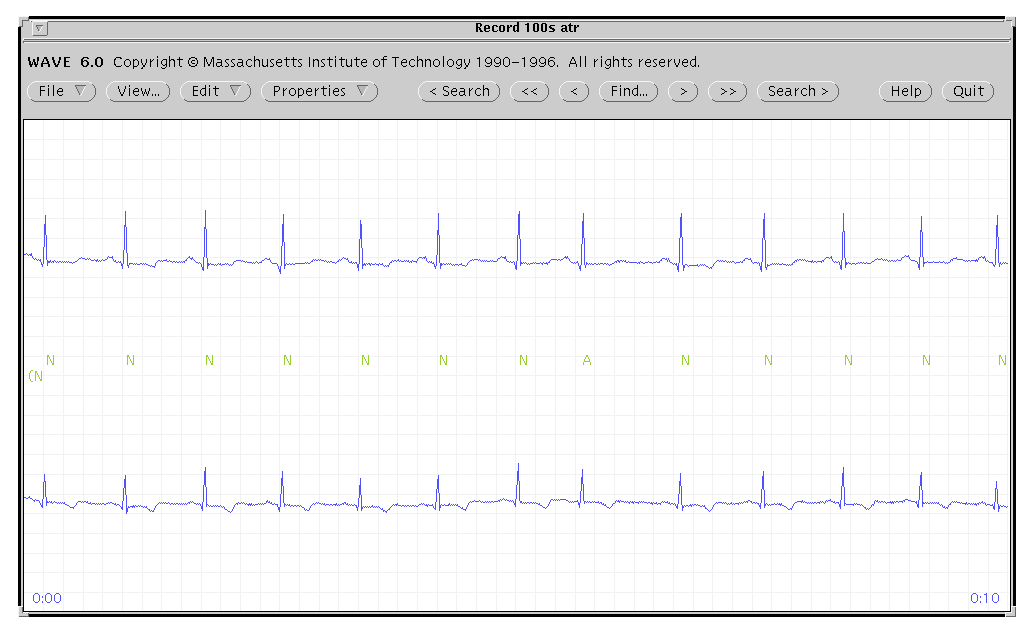
\epsfig{file=main-window.ps}}
\caption{\WAVE{}'s main window.}
\begin{htmlonly}
\index{main window}
\end{htmlonly}
\begin{latexonly}
\index{main window|textbf}
\end{latexonly}
\label{fig:main-window}
\end{figure}

\subsection*{A Five-Minute Tour of \WAVE{}}

At the top of the window is the \emph{title bar},
\begin{htmlonly}
\index{title bar}\index{window!title bar}
\end{htmlonly}
\begin{latexonly}
\index{title bar|emph}\index{window!title bar|emph}
\end{latexonly}
which reads `{\sf Record 100s atr}'.  Below the title bar is \WAVE{}'s
\emph{main control panel},
\begin{htmlonly}
\index{main control panel}
\end{htmlonly}
\begin{latexonly}
\index{main control panel|emph}
\end{latexonly}
which contains three groups of buttons.  Several of these (\menubutton{File},
\menubutton{Edit}, and \menubutton{Properties}) are \emph{menu buttons}
(distinguished by the `$\nabla$' at the right end of the button), and are
selectable using the right mouse button.  The other buttons are selected using
the left mouse button.

\begin{htmlonly}
\index{signal!window}
\end{htmlonly}
\begin{latexonly}
\index{signal!window|emph}
\end{latexonly}
Below the main control panel is the \emph{signal window}.
This window shows a
portion of the sample record {\tt 100s}, which contains two signals.
Between the two signals, \emph{annotations} are shown.
The first annotation (`{\sf (N}', at
the left edge of the window) is shown below the level of the others, to
indicate that it is a rhythm label
\index{rhythm label}\index{annotation!rhythm}
(`{\sf (N}' means normal sinus rhythm).
Most of the other annotations are `{\sf N}', and indicate normal beats; the
`{\sf A}' indicates an atrial premature beat.  In the lower corners of the
signal window, the \emph{time indicators}
\begin{htmlonly}
\index{time indicator}
\end{htmlonly}
\begin{latexonly}
\index{time indicator|emph}
\end{latexonly}
(`{\sf 0:00}' and `{\sf 0:10}') show the
elapsed time in minutes and seconds from the beginning of the record to the
samples at the left and right edges of the window respectively.  (If your
display is less than about 260 mm wide, the signal window will not show a full
10 seconds of the record.)  When you move the pointer into the signal window,
it changes shape.  Annotation editing and other operations are possible while
the pointer is in the signal window; these operations are described in later
exercises.

The buttons in the middle group (\button{{\tt <} Search}, \button{\tt <<},
\button{\tt <}, \button{Find...}, \button{\tt >}, \button{\tt >>}, and
\button{Search {\tt >}}) are the controls
\index{controls!navigation}\index{navigation controls}
\index{moving through a record}
that you use to navigate
through the record.  The \button{\tt >>} button advances the signal window
display by the width of the window (10 seconds in this case).  Move
the mouse pointer over \button{\tt >>} and press the left button.
(This common action is referred to below as `clicking left on \button{\tt
>>}'.)  The signal window is redrawn, and now shows the interval from
0:10 to 0:20.  The \button{\tt >} button also advances the window, but by
only half the window width.  Try it now.  Similarly, \button{\tt <<}
moves the window back by one screenful, and \button{\tt <}
moves it back by half a screenful.  Use these buttons to move to a
window that begins at 0:55.  Since the record is only 1 minute long,
the right half of the window is empty.  Notice that you can continue
to advance past the end of the record if you wish.  (\WAVE{} will
not allow you to back up past the beginning of the record, however.)

Buttons such as \button{Find...}, with labels that end with `{\sf ...}', make
\WAVE{} open other (so-called `pop-up') windows.
\index{pop-up windows}
Click left on
\button{Find...} now.  The {\sf Find} window (figure~\ref{fig:find-window})
will appear.
\begin{figure}
\centerline{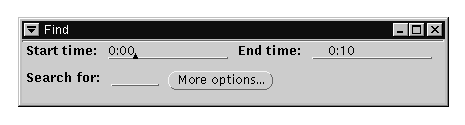
\epsfig{file=find-window.ps}}
\caption{The {\sf Find} window.}
\begin{htmlonly}
\index{Find window@{\sf Find} window}
\end{htmlonly}
\begin{latexonly}
\index{Find window@{\sf Find} window|textbf}
\end{latexonly}
\label{fig:find-window}
\end{figure}
Its location on your screen is controlled by your window manager; typically it
will appear either at the upper-left corner of the screen, or directly beneath
the pointer (obscuring part of the signal window).  If you wish, move the
{\sf Find} window to another location on your screen.

Within the {\sf Find} window are three text fields in which you may type.
Move the pointer into the the part of the window below the title bar.
A black, upward-pointing triangle (the text cursor
\begin{htmlonly}
\index{text cursor}
\end{htmlonly}
\begin{latexonly}
\index{text cursor|emph}
\end{latexonly}
or \emph{insertion point})
\index{insertion point}
should appear in one of the three
fields.  (Once again, your window manager may influence what you see.
If you see a grey diamond rather than a black triangle, you must
perform whatever action your window manager requires to give the
\emph{keyboard focus}
\begin{htmlonly}
\index{keyboard focus}
\end{htmlonly}
\begin{latexonly}
\index{keyboard focus|emph}
\end{latexonly}
to the {\sf Find} window.  Usually, clicking left is
sufficient.)

The {\sf Start time}
\index{start time@{\sf Start time}}
and {\sf End time}
\index{end time@{\sf End time}}
fields match the times shown
in the lower corners of the signal window.  If you change either of
these fields, the signal window moves accordingly.  To change a text
field, move the pointer to the right of the existing text and click
left, press \keycap{Backspace} or \keycap{DEL} to erase any characters
you wish to change, and type in the desired value, finishing by
pressing \keycap{Enter} (or \keycap{Return}).  (Always remember to
press \keycap{Enter} after changing a text field; your changes are not
registered until you press \keycap{Enter}.)  Try changing the {\sf
Start time} and {\sf End time} fields now, and watch how the contents
of the signal window change.  You can type any desired time into these
fields; specifically, it need not be a multiple of 5 seconds.

Using any of the controls you have seen so far, set the signal window
so that it shows the segment of the record beginning at 0:22.  Now
select the {\sf Search for}
\index{search}\index{annotation!searching for}
field, and enter `{\tt A}' (followed, as
always, by \keycap{Enter}).  This action asks \WAVE{} to find the
next occurrence of an `{\sf A}' (atrial premature beat) label, and to
redraw the signal window roughly centered on that label.  As you may
have noticed, the only `{\sf A}' annotation in record {\tt 100s}
occurs at about 0:06, so \WAVE{} is unable to satisfy this request.
Whenever \WAVE{} cannot do what you have asked, it displays
\begin{wrapfigure}[7]{r}{3cm}
\mbox{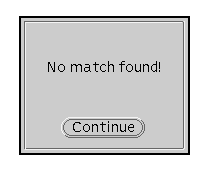
\epsfig{file=nomatch.ps}}
\begin{htmlonly}
\index{notice box}
\end{htmlonly}
\begin{latexonly}
\index{notice box|textbf}
\end{latexonly}
\end{wrapfigure}
a \emph{notice box},
\marginpar{\emph{In \WAVE{} 5.0, notice boxes
perform a so-called `full screen grab',
\index{full screen grab, in \WAVE{} 5.0}
which prevents mouse or keyboard
events from being delivered to any other window, including those that
belong to other applications.}}
with a brief message describing what has happened.
(In this case, the message is `{\sf No match found!}', in other words,
there are no `{\sf A}' labels between 0:32 and the end of the record.)
Notice boxes are usually accompanied by a beep (although your window
manager may allow you to disable the beep).  Notice boxes
always contain at least one button (in this case, labelled
\button{Continue}).  When a notice box is displayed, you \emph{must}
click left on one of the buttons in the notice box before you can do
anything else in \WAVE{}.
Click left on \button{Continue} now to
dismiss the notice box.

\index{search}\index{annotation!searching for}
The \button{{\tt <} Search} and \button{Search {\tt >}} buttons on
\WAVE{}'s main control panel are used to search for annotations
that match the {\sf Search for} field in the Find window.  Searching
forward using \button{Search {\tt >}} will be unsuccessful (we know
this, because \WAVE{} has already tried to do so after we changed
the contents of the {\sf Search for} field).  Use \button{{\tt <}
Search} button to search backwards.  The signal window now shows the
segment from 0:01 to 0:11, with the `{\sf A}' annotation at 0:06
roughly centered in the window.  If you use either \button{{\tt <}
Search} or \button{Search {\tt >}} now, the search fails, because the
only `{\sf A}' annotation in the record is already on-screen.  For
more information, see
\hyperref{Searching for annotations}
{section~}
{, page~\pageref{sec:searching}}
{sec:searching}.

\begin{wrapfigure}{l}{2.2cm}
\mbox{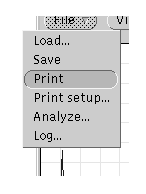
\epsfig{file=file-print.ps}}
\end{wrapfigure}
\index{printing!signal window contents}\index{screen dump}
\index{PostScript}
\index{SPARCprinter}
If a PostScript printer is available, try printing the contents of the
signal window.  To do this, press and hold the right mouse button
while the pointer is above \menubutton{File}; then drag the pointer
downwards until the {\sf Print} selection is
highlighted, and release
the right mouse button.  Printing will require between 20 seconds (if
you have a SPARCprinter) and several minutes (if you have a typical
PostScript printer); it is not necessary to wait for the output to
appear before continuing.  The output will appear as in
figure~\ref{fig:chart1}.
\begin{figure}
\fbox{\centerline{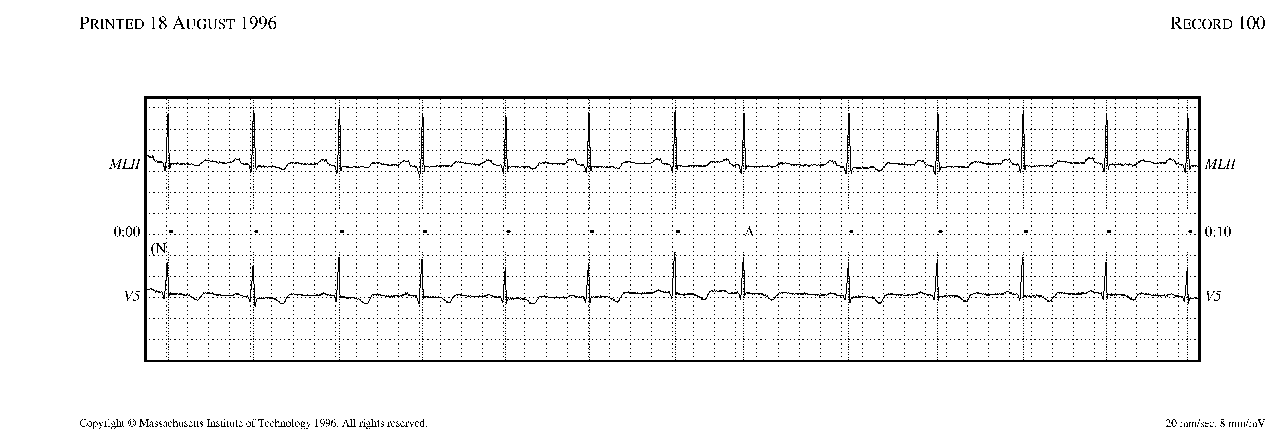
\epsfig{file=chart1.ps,angle=-90,width=.9\linewidth}}}
% This figure was produced in ``landscape'' mode.  To print it
% properly in portrait mode, it must be rotated by -90 degrees
% *before* scaling it.
\caption{Printed ``chart recording'' made using {\sf Print} from the
{\sf File} menu.}
\label{fig:chart1}
\end{figure}

\WAVE{} has three types of on-line help.
\index{help}\index{on-line help}
The first type, called \emph{spot help},
\begin{htmlonly}
\index{spot help}\index{Open Look!spot help}
\end{htmlonly}
\begin{latexonly}
\index{spot help|emph}\index{Open Look!spot help|emph}
\end{latexonly}
works properly only if you are using an Open Look
window manager ({\tt olwm} or {\tt olvwm}),
\index{olwm@{\tt olwm} (Open Look Window Manager)}
\index{olvwm@{\tt olvwm} (Open Look Virtual Window Manager)}
although a local expert may
be able to show you how to use it with another window manager.  To
use spot help with an Open Look window manager, move the pointer to
any control or display area in a \WAVE{} window and press the
\keycap{HELP} key (or the \keycap{F1} key if your keyboard does not
have a \keycap{HELP} key).  A \emph{spot help window} (see
figure~\ref{fig:spot-help}) 
\begin{htmlonly}
\index{help window}
\end{htmlonly}
\begin{latexonly}
\index{help window|emph}
\end{latexonly}
appears; it contains a
magnifying glass icon showing the area you have selected, and a
description of the control or display.
\begin{figure}
\centerline{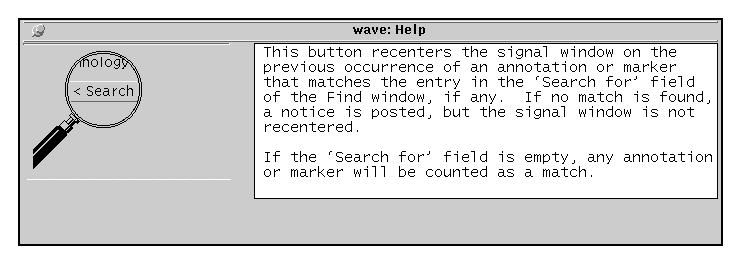
\epsfig{file=spot-help.ps}} \caption{A spot help window.}
\index{spot help}
\begin{htmlonly}
\index{Open Look!spot help}
\end{htmlonly}
\begin{latexonly}
\index{Open Look!spot help|textbf}
\end{latexonly}
\label{fig:spot-help}
\end{figure}

To get an overview of how to use \WAVE{}, or if you cannot use spot help,
click left on \button{Help} in \WAVE{}'s main control panel.
\begin{figure}
\centerline{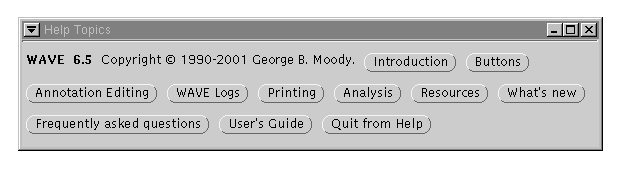
\epsfig{file=help-topics.ps}}
\caption{The {\sf Help Topics} window.}
\begin{htmlonly}
\index{Help Topics window@{\sf Help Topics} window}
\end{htmlonly}
\begin{latexonly}
\index{Help Topics window@{\sf Help Topics} window|textbf}
\end{latexonly}
\label{fig:help-topics}
\end{figure}
The {\sf Help Topics} window (see figure~\ref{fig:help-topics})
appears, from which you may select any of the
available topics by clicking left on the corresponding button.  If you do so, a
scrollable \emph{help text window} (see figure~\ref{fig:help-text})
appears, containing information on the selected topic.
\begin{figure}
\centerline{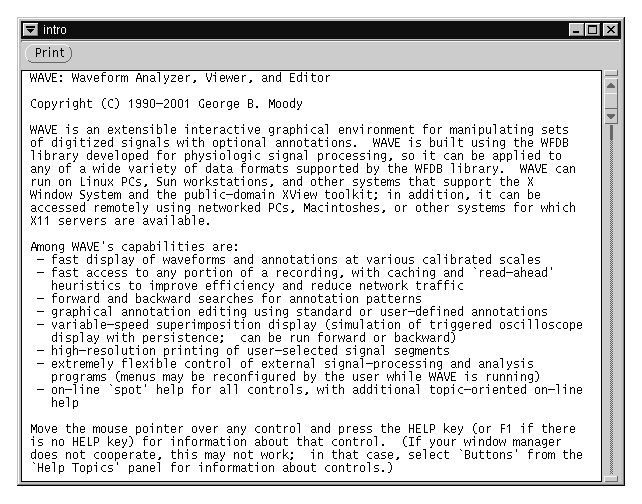
\epsfig{file=help-intro.ps}}
\caption{A help text window.}
\begin{htmlonly}
\index{help text window}\index{window!help text}
\end{htmlonly}
\begin{latexonly}
\index{help text window|textbf}\index{window!help text|textbf}
\end{latexonly}
\label{fig:help-text}
\end{figure}
Scroll up and down through the window by clicking left on the black
triangles in the scroll bar (or use any other Open Look methods if you
are familiar with them).  If you wish, you can click left on the
\button{Print}
\index{printing!on-line help}\index{help!printing}
\marginpar{\emph{These \button{Print} buttons are not available in \WAVE{}
5.0.}}
button at the top of the window to obtain a paper copy.
Dismiss the window by clicking right on the \emph{window menu button}
\index{window!menu button}\index{closing windows}
(the square button containing a triangle at the upper left corner of the
window), and then clicking left on the {\sf Quit} item in the window
menu.

\index{Netscape}\index{web browsers}
\index{on-line manual}\index{User's Guide (on-line)}
\index{WAVE User's Guide (on-line)@\WAVE{} User's Guide (on-line)}
The third (and most comprehensive) form of on-line help can be used if
a suitable web browser is available on the \WAVE{} host system.
(\WAVE{} uses Netscape 1.1 or any later version by default.  See
\hyperref{\WAVE{} and the Web}
{section~}
{, page~\pageref{sec:web},}
{sec:web}
for details on obtaining Netscape, or on configuring \WAVE{} to use a
different web browser.)
Click left on the \button{WAVE User's Guide} button in the {\sf Help
Topics} window to open this manual using your web browser.  If your
browser is not running already, this may take a few moments while
\WAVE{} starts it up.

\begin{wrapfigure}[7]{r}{4.75cm}
\mbox{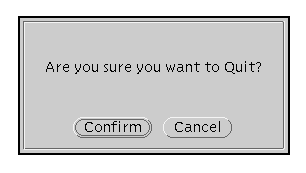
\epsfig{file=notice-quit.ps}}
\end{wrapfigure}
To complete this exercise, exit from \WAVE{} by clicking left on
\button{Quit} in \WAVE{}'s main control panel.  A notice box
\index{Quit button@{\sf Quit} button}
appears as shown at right; click
left on \button{Confirm} to exit, or on \button{Cancel} if you're
having so much fun that you don't want to stop yet.  Once you have
exited from \WAVE{}, log off of the \WAVE{} host
\index{WAVE host@\WAVE{} host}
(and your own computer, if you have been running a remote copy of \WAVE{}).

\chapter{Annotation Editing}

There are five editing operations that you can perform using \WAVE{}:
changing, moving, copying, inserting, and deleting annotations.  In
this chapter, you will create and edit an annotation file using \WAVE{}
and an external QRS detection program.  Start as in the previous
chapter, but use the command
\begin{verbatim}
    wave -r 100s &
\end{verbatim}
omitting the `{\tt -a atr}' option this time.  Note that the title bar
contains only the record name.

\begin{wrapfigure}[9]{l}{2.2cm}
\mbox{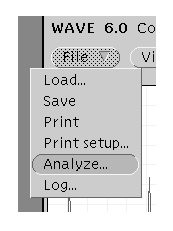
\epsfig{file=file-analyze.ps}}
\end{wrapfigure}
Click right on \menubutton{File}, and click left on the {\sf Analyze...}
selection in the File menu.  After a short delay, the {\sf Analyze}
window (see figure~\ref{fig:analyze-window}) and the
{\sf Analysis Commands} window (see figure~\ref{fig:analysis-commands}) appear.
\begin{figure}
\centerline{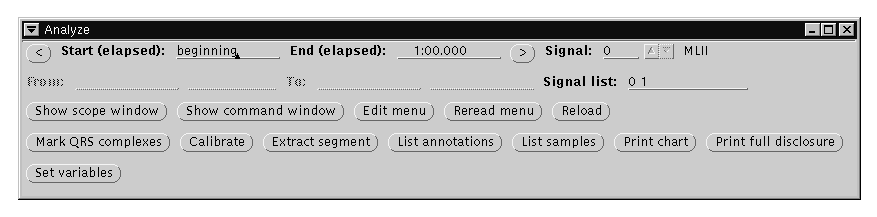
\epsfig{file=analyze-window.ps}}
\caption{The {\sf Analyze} window.}
\begin{htmlonly}
\index{Analyze window@{\sf Analyze} window}
\end{htmlonly}
\begin{latexonly}
\index{Analyze window@{\sf Analyze} window|textbf}
\end{latexonly}
\label{fig:analyze-window}
\end{figure}
At any time, you can click on \button{Show command window} in the {\sf Analyze}
window to make the {\sf Analysis Commands} window visible if it becomes
covered by another window.

Below the title bar of the {\sf Analyze} window, text fields allow you to
specify the beginning and end of a segment of the record, and to
choose signals.  The {\sf Analyze} window also contains buttons specifying
various actions that you can apply to the signals.  The separate
{\sf Analysis Commands} window behaves like an OpenWindows {\tt cmdtool}
\index{cmdtool@{\tt cmdtool}}
\begin{figure}
\centerline{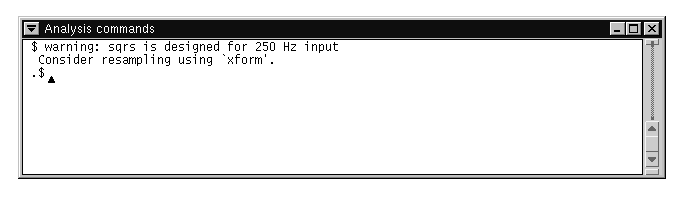
\epsfig{file=analysis-commands.ps}}
\caption{The {\sf Analysis Commands} window.}
\begin{htmlonly}
\index{analysis commands window@{\sf Analysis Commands} window}
\end{htmlonly}
\begin{latexonly}
\index{analysis commands window@{\sf Analysis Commands} window|textbf}
\end{latexonly}
\label{fig:analysis-commands}
\end{figure}
window (a scrollable terminal emulator).  Commands may be run in the
{\sf Analysis Commands} window either by clicking left on action buttons
\index{action buttons}
in the {\sf Analyze} window, or by typing directly into the window (depending
on your window manager's policy for moving the keyboard focus, you may
need to click left within the window before you can type into it,
however).  The {\sf Analysis Commands} window may be resized if desired, and
standard Open Look user interface methods may be used to cut and paste
text between it and other windows, including those in other
applications.

To create an annotation file,
\index{annotation file!creating!using an external program}
\index{creating an annotation file!using an external program}
click left on \button{Mark QRS complexes}.
The command
\begin{verbatim}
    sqrs -r 100s -f 0 -t 1:00.000 -s 0
\end{verbatim}
appears in the {\sf Analysis Commands} window, as shown in
figure~\ref{fig:analysis-commands}.  Below the command, its error
output appears.  When the command has run to completion (which will take only
a few seconds unless the \WAVE{} host is heavily loaded), an annotation file
named `{\tt qrs.100s}' is written into the current directory.

If you wish, the {\sf Analyze} window or the {\sf Analysis Commands}
window, or both, may be dismissed (by selecting {\sf Quit} from the
window menu to the left of the title bar); this can be done at any
time, even while analysis is still in progress.  If you recall the
{\sf Analysis Commands} window later (using \button{Show command window}
in the {\sf Analyze} window), it will show any output sent to it
while it was dismissed.  Note that the {\sf Analysis Commands} window is
dismissed whenever you exit from \WAVE{}, and its contents are not
retained after that point.

\section{Loading annotations to be edited}
\begin{wrapfigure}[8]{l}{2.2cm}
\mbox{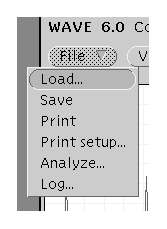
\epsfig{file=file-load.ps}}
\end{wrapfigure}
To load annotations
\index{annotation file!loading}\index{loading an annotation file}
from `{\tt qrs.100s}' into \WAVE{}, click right on
\menubutton{File}, and click left on the {\sf Load...} selection in the
File menu.
\begin{figure}
\centerline{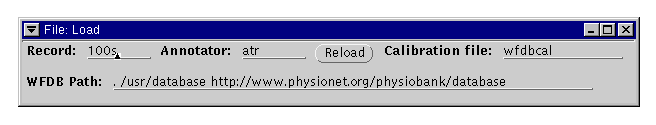
\epsfig{file=load-window.ps}}
\caption{The {\sf Load} window.}
\begin{htmlonly}
\index{Load window@{\sf Load} window}
\end{htmlonly}
\begin{latexonly}
\index{Load window@{\sf Load} window|textbf}
\end{latexonly}
\label{fig:load-window}
\end{figure}
The {\sf Load} window (see figure~\ref{fig:load-window}) appears.  It
contains text items that specify a
record and and an annotator name.  Click left next to the {\sf
Annotator} field, type `{\tt qrs}', and, as always, press \keycap{
Enter}.  The contents of `{\tt qrs.100s}' are loaded into \WAVE{}, and
annotations appear in the signal window.  The title bar
\index{title bar}
changes to indicate the annotator name.
\index{annotator name}
The {\sf Load} window also contains items that specify the name of the
calibration file
\index{calibration file}
\index{database path;}
and the
\hyperref{database path}
{database path (see section~}
{, page~\pageref{sec:wfdb-path});}
{sec:wfdb-path}
you will not need to change these items for this exercise.  You may
dismiss the {\sf Load} window or leave it up as you wish.

If you have looked through the record using the navigation buttons,
use them now to return to the beginning of the record.  The time
indicator in the lower left corner of the signal window should read
`{\sf 0:00}'.  Since the \button{Mark QRS complexes} button only
produces `{\sf N}' (normal) beat labels, the eighth beat in the window
(an atrial premature beat) is mislabelled.  In the next part of this
exercise, we will correct this label.

\section{The {\sf Annotation Template}}
Move the pointer into the signal window and click left.  \WAVE{}'s
{\sf Annotation Template} window appears (see
figure~\ref{fig:annotation-template}).
\begin{figure}
\centerline{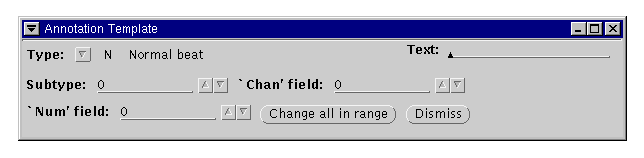
\epsfig{file=annotation-template.ps}}
\caption{The {\sf Annotation Template} window.}
\begin{htmlonly}
\index{Annotation Template window@{\sf Annotation Template} window}
\end{htmlonly}
\begin{latexonly}
\index{Annotation Template window@{\sf Annotation Template} window|textbf}
\end{latexonly}
\label{fig:annotation-template}
\end{figure}
The contents of the {\sf Annotation Template} window indicate what
type of annotation will be inserted if you decide to insert an
annotation.  Click right on the \amenubutton{Type:} abbreviated
menu button.  The {\sf Type} menu
\index{Type menu@{\sf Type} menu}
appears (see figure~\ref{fig:type-menu}).
\begin{figure}
\centerline{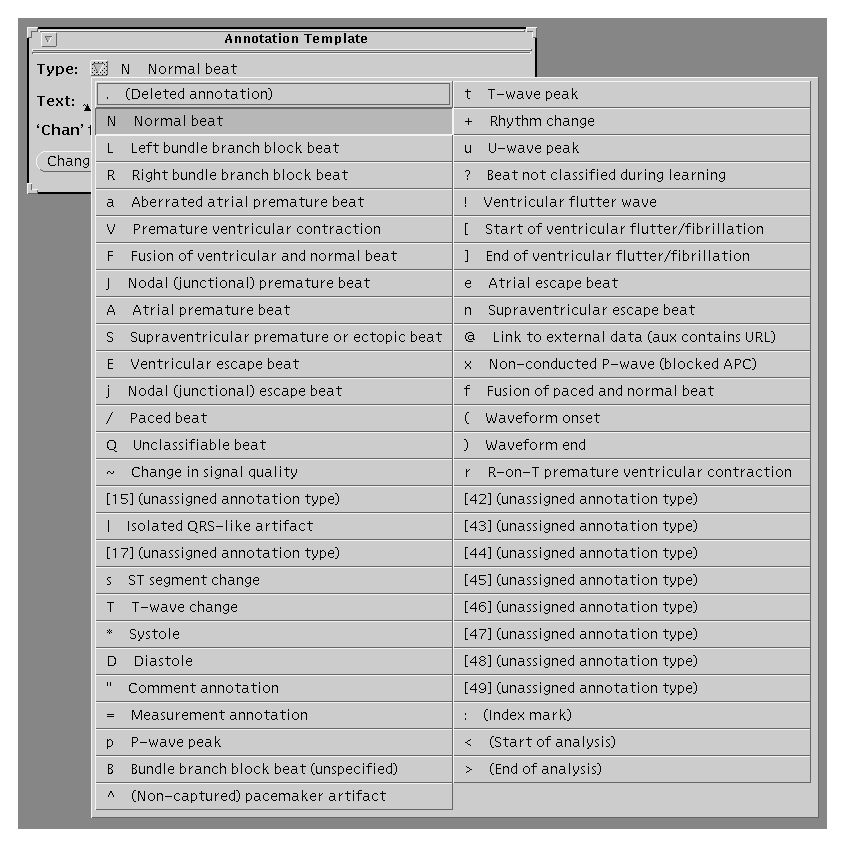
\epsfig{file=type-menu.ps}}
\caption{The {\sf Type} menu.}
\label{fig:type-menu}
\begin{htmlonly}
\index{Type menu@{\sf Type} menu}
\end{htmlonly}
\begin{latexonly}
\index{Type menu@{\sf Type} menu|textbf}
\end{latexonly}
\end{figure}
Select `{\sf A~Atrial premature beat}' from the {\sf Type} menu by
clicking left on it.  This action dismisses the {\sf Type} menu, and
your selection now appears in the {\sf Annotation Template} window to
the right of the \amenubutton{Type:} menu button.  The other
fields of the {\sf Annotation Template} can be ignored for this exercise.

Single-character annotation mnemonics
\index{annotation!mnemonic}
that appear in the {\sf Annotation Template}'s {\sf Type} menu
can be used as shortcuts 
\index{editing shortcuts}
during annotation editing.  (These mnemonics are the same as those used by
\WAVE{} to indicate annotations in the signal window.)  Instead of
calling up the {\sf Type} menu, you may
simply type the mnemonic at any time while the pointer is in the
signal window, provided that the {\sf Annotation Template} window is open.
If you type a recognized mnemonic, the {\sf Annotation Template} is updated
immediately to reflect your choice.

\begin{wrapfigure}[8]{r}{6.3cm}
\mbox{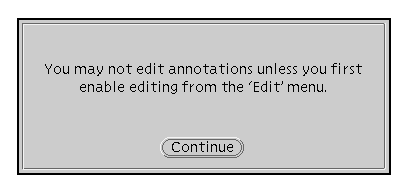
\epsfig{file=noedit.ps}}
\end{wrapfigure}
Annotation editing
\index{annotation!enabling editing}
is disabled by default, to avoid inadvertent modification
of annotation files.  If you now move the pointer into the signal window and
click the middle button, this action is understood to mean that you wish to
insert an annotation of the type shown in the {\sf Annotation Template} at the
location indicated by the pointer.  Since \WAVE{} cannot satisfy this
request until annotation editing has been enabled, a notice box (shown above)
appears to warn you that no
action has been taken.  Click left on \button{Continue} to dismiss the
notice box.

\begin{wrapfigure}{l}{3cm}
\mbox{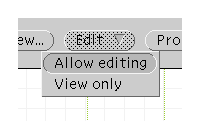
\epsfig{file=allow-edit.ps}}
\begin{htmlonly}
\index{Edit menu@{\sf Edit} menu}
\end{htmlonly}
\begin{latexonly}
\index{Edit menu@{\sf Edit} menu|textbf}
\end{latexonly}
\end{wrapfigure}
To enable annotation editing, click right on \menubutton{Edit},
and click left on the {\sf Allow editing} selection in the {\sf Edit}
menu.  (Your selection from the {\sf Edit} menu persists for the duration of
your {\sf WAVE} session, unless you return to the {\sf Edit} menu to change
it.  Thus it is sufficient to enable annotation editing once if you plan to
edit several records in a single session.)

\section{Selecting an annotation}
\label{sec:selecting-annotation}
In this case, we need to change an existing `{\sf N}' annotation into
an `{\sf A}' annotation.  To do so, we must select the annotation to
be changed.
\index{annotation!selecting}
Annotations are selected by clicking left or right in the
signal window.  Whenever the pointer is in the signal window, clicking
left selects the annotation to the left of the pointer, and clicking
right selects the annotation to the right of the pointer.  (If `Num
Lock' is off, and the pointer is within the signal window, you can use
the \keycap{$\leftarrow$} or \keycap{$\rightarrow$} keys
\marginpar{\emph{The arrow keys cannot be used in \WAVE{} 5.0.}}
instead of the mouse buttons if you prefer.)  The annotation is highlighted by
a \emph{selection rectangle}
\begin{htmlonly}
\index{selection rectangle}
\end{htmlonly}
\begin{latexonly}
\index{selection rectangle|emph}
\end{latexonly}
drawn around it, and the pointer jumps to
the center of the rectangle (see figure~\ref{fig:main-with-markers}).
\begin{figure}
\centerline{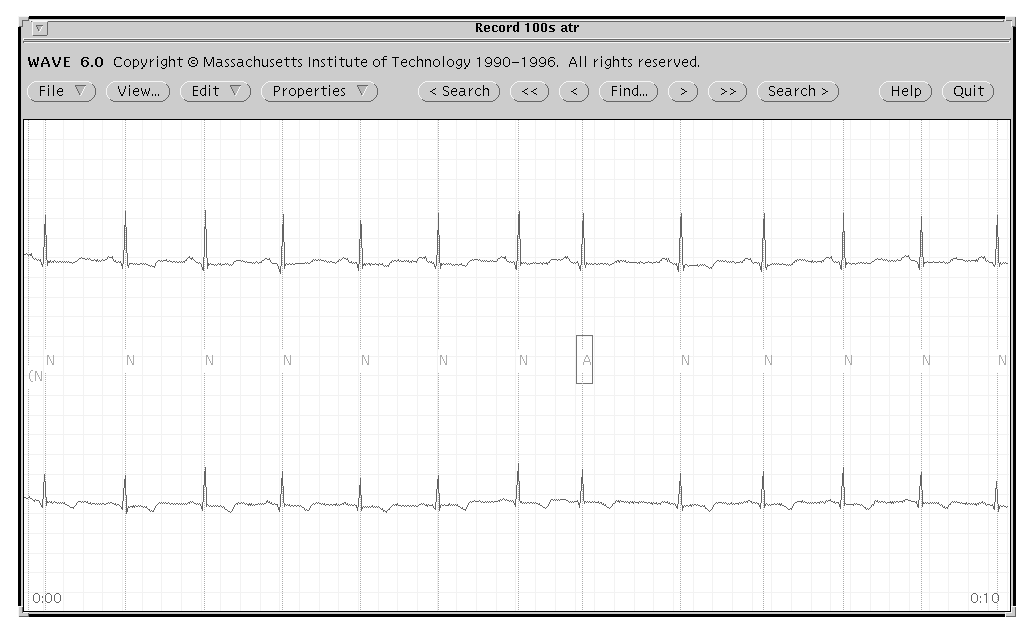
\epsfig{file=main-with-markers.ps}}
\caption{The main window, showing the selection rectangle and marker bars.}
\begin{htmlonly}
\index{selection rectangle}
\index{marker bars}
\end{htmlonly}
\begin{latexonly}
\index{selection rectangle|textbf}
\index{marker bars|textbf}
\end{latexonly}
\label{fig:main-with-markers}
\end{figure}
If clicking left or right would otherwise move the pointer out of the signal
window, \WAVE{} recenters the signal window on the selected annotation.
While any of the mouse buttons is down, \emph{marker bars}
\index{marker bars}
appear above and
below the pointer to allow you to identify the pointer location with respect to
the signals.

It is often useful, especially while editing annotations, to display marker
bars above and below \emph{each} annotation.  If you wish to do so, click left
on \button{View...}, then click left on the \keycap{markers} selection
in the {\sf View} window that appears (see
figure~\ref{fig:view-window}), and finally click left on
\button{Redraw} to dismiss the {\sf View} window and redraw the signal window
with annotation marker bars (see figure~\ref{fig:main-with-markers}).
\begin{figure}
\centerline{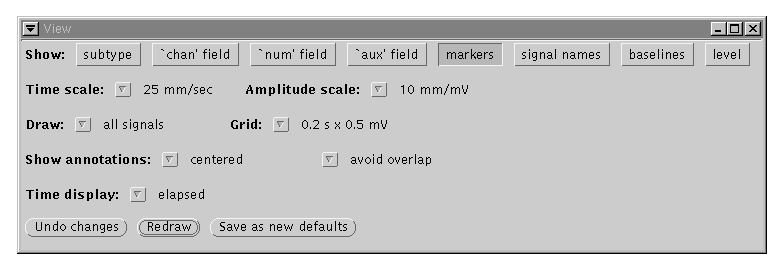
\epsfig{file=view-window.ps}}
\caption{The {\sf View} window.}
\label{fig:view-window}
\begin{htmlonly}
\index{View window@{\sf View} window}
\end{htmlonly}
\begin{latexonly}
\index{View window@{\sf View} window|textbf}
\end{latexonly}
\end{figure}
The marker bars can be turned off by repeating this procedure.

\section{Changing an annotation without moving it}

\index{annotation!changing without moving}\index{changing an annotation}
Select the eighth beat label by clicking left or right, or using the
arrow keys, until the selection rectangle surrounds it.  Change the
`{\sf N}' to an `{\sf A}' by clicking the middle button or pressing
\keycap{F2}.
\marginpar{\emph{\keycap{F2} and \keycap{5} can't be used in \WAVE{} 5.0.}}
(On some keyboards, if `Num Lock' is off, you can use the \keycap{5} key on
the numeric keypad instead of \keycap{F2} if you prefer.)  The `{\sf N}' is
\begin{wrapfigure}[4]{r}{3cm}
\mbox{
\epsfig{file=title-with-parens.ps}}
\begin{htmlonly}
\index{title bar!parentheses in}
\end{htmlonly}
\begin{latexonly}
\index{title bar!parentheses in|textbf}
\end{latexonly}
\end{wrapfigure}
replaced by an `{\sf A}' and the selection rectangle disappears.  To
indicate that there are unsaved edits in the annotation file, the
\index{annotator name}
annotator name in \WAVE{}'s main window title bar is marked by
parentheses.

\section{Moving an annotation}

\index{annotation!moving}\index{moving an annotation}
Although no further editing should be necessary, try out the other editing
operations now.  To move an annotation, select it with the left or right
button, drag its marker bars (with the left or right button still depressed)
to the desired location, then release the mouse button to drop the annotation.
The selection rectangle stays in the original location
until the button is released, but the marker bars move with the pointer once
the pointer moves outside of the rectangle.  To move an annotation by less than
the width of the rectangle, simply drag the pointer above or below the
rectangle.

\marginpar{\emph{These keyboard commands are not available in \WAVE{}
5.0.}}
\index{keyboard commands}
If you prefer, you may use the keyboard rather than the mouse for this
operation.  To do so, drag the marker bars left or right using
\keycap{F3} or \keycap{F4}, and then drop the annotation using \keycap{F2}.

If you change your mind about moving an annotation, drag the pointer
back into the selection rectangle, and then drop the annotation.

\section{Inserting an annotation}

\index{annotation!inserting}\index{inserting an annotation}
To insert an annotation, move the pointer into the signal window (but outside
of the selection rectangle if it is visible), press the middle button, drag the
marker bars to the desired location, and release the middle button to complete
the insertion.

\section{Copying an annotation}

\index{annotation!copying}\index{copying an annotation}
\marginpar{\emph{This feature is not available in \WAVE{} 5.0.}}
To copy an annotation, select it, then press the \keycap{Copy} key (or
\keycap{F6} if your keyboard does not have a \keycap{Copy} key).  This
action copies the selected annotation into the {\sf Annotation Template}.
Now insert the copy at the desired location.  (This is a particularly
useful shortcut if you are working with complex annotations for which
fields other than the {\sf Type} must be set.)

\section{Deleting and restoring annotations}

\index{annotation!deleting}\index{deleting an annotation}
\index{annotation!restoring deleted}\index{restoring a deleted annotation}
\index{undeleting an annotation}\index{finding deleted annotations}
\index{locating deleted annotations}\index{search!for deleted annotations}
To delete an annotation, first click right on the {\sf Annotation
Template} window's \amenubutton{Type:} menu button, and select `{\sf .
(deleted annotation)}', the first entry.  Now select the annotation to
be deleted by clicking left or right in the signal window, and click
the middle button to delete it.  The annotation is replaced by a `{\sf
.}' marker, which remains in \WAVE{}'s annotation buffer until a
new annotation file is read or until you exit from \WAVE{}.  This
feature allows you to locate deleted annotations if necessary (you may
search for them by entering `{\tt .}' in the {\sf Search for} field of
the {\sf Find} window;  see
\hyperref{Searching for annotations}
{section~}
{, page~\pageref{sec:searching}}
{sec:searching}).
To restore a deleted annotation, simply repeat the operations that you
used to delete it.

\section{Markers}

The `{\sf .}' that appears when you delete an annotation is an example
of a \emph{marker}.
\begin{htmlonly}
\index{marker}
\end{htmlonly}
\begin{latexonly}
\index{marker|emph}
\end{latexonly}
The important difference
between \emph{markers} and \emph{annotations}
\index{annotation!vs. marker}
is that markers are never written to
annotation files; they remain in \WAVE{}'s annotation buffer only
until \WAVE{} reads another annotation file, or until you exit from
\WAVE{}, whichever comes first.  Other types of markers are `{\sf :}'
(index marks,
\index{index mark}
which you may insert anywhere in a
record, and which you can return to by searching for them), `{\tt <}'
(beginning of region), and `{\tt >}' (end of region).
\index{beginning of region}\index{end of region}\index{region of interest}
The `{\tt <}' and `{\tt >}' markers are special in that only
one of each may be defined at any time; inserting a new one deletes
the old one, if any.  If the {\sf Analyze} window
\index{Analyze window@{\sf Analyze} window}
is visible, you will notice that
inserting or moving the `{\tt <}' marker has the effect of changing
the contents of the {\sf Start (elapsed)} field (and the {\sf From}
field, if it is enabled); another way to insert a `{\tt <}' marker is
to enter the desired time directly into the {\sf Start (elapsed)}
field.  The `{\tt >}' marker is similarly coupled with the {\sf End
(elapsed)} field (and the {\sf To} field) of the {\sf Analyze} window.

\section{Changing the {\sf Annotation Template}}

\WAVE{} maintains a record of several of the most recently used settings
in the
\marginpar{\emph{This feature is not available in \WAVE{} 5.0.}}
{\sf Annotation Template} (this information is not saved when
you exit \WAVE{}, however).  You can cycle through these settings if you
have a three-button mouse; to do so, press and hold the middle button
as if to insert an annotation, then click left or right to change the
contents of the {\sf Annotation Template}.  (If you don't wish to
insert an annotation, release the middle button before releasing the
left or right button.)  This feature is particularly useful if you are
manually annotating a record and you find it necessary to use a small
number of different annotations to do so.

\section{Changing many annotations at once}

\index{annotation!changing many at once}\index{changing many annotations}
The usual method for changing annotations (clicking right or left to select the
annotation to be changed, then clicking the middle button to perform the
change) can become tedious if you have many annotations to change.  \WAVE{}
offers a shortcut
\index{shortcut}
if you wish to change all annotations in a specified region
in the same way.  First, specify the region by inserting a `{\tt <}' marker
before the first annotation to be changed, and a `{\tt >}' marker after the
last annotation to be changed.  Next, fill in the {\sf Annotation Template} to
indicate how you wish to change the annotations in the region.  Finally, click
left on \button{Change all in range}.  (If the region includes any
annotations that are not visible on-screen, \WAVE{} prompts you to confirm
that you wish to change them.)  Try out this technique now.  Insert the `{\tt
<}' marker at 0:15, the `{\tt >}' marker at 0:30, and change all of the
annotations in the region to type `{\sf V}' (premature ventricular
contraction).  Inspect the results, then change them back to `{\sf N}'
annotations.

\section{Searching for annotations}

\label{sec:searching}
\WAVE{} can search in either direction for the next annotation that
meets criteria you specify using the {\sf Search for} field in the
{\sf Find} window.  Any string that \WAVE{} displays as an annotation
label can be entered into the {\sf Search for} field as a search
criterion;  these strings include annotation and marker mnemonics
(usually single characters;  see the {\sf Type} menu for a list),
signal quality strings (these contain one or more characters from the set
``{\tt c}'', ``{\tt n}'', and ``{\tt u}''; ``{\tt U}'' is also a legal
signal quality annotation), and {\em any substring} within a note,
rhythm change, ST or T change, or link annotation.  In addition to
these, there are several {\sf Search for} strings that \WAVE{}
interprets in special ways:

\begin{tabular*}{\textwidth}{l p{3.5 in}}
{\tt *v} & {matches any ventricular ectopic beat} \\
{\tt *s} & {matches any supraventricular ectopic beat} \\
{\tt *n} & {matches any other beat type} \\
{\tt *}  & {matches any annotation or marker} \\
{\tt .}  & {matches a deletion made during this \WAVE{} session} \\
\end{tabular*}

More complex search criteria can be defined by clicking on
\button{More Options...} in the {\sf Find} window.  This opens the
{\sf Search Template} window (figure~\ref{fig:search-template}).
\marginpar{\emph{The {\sf Search Template} is not available in \WAVE{}
5.0.}}
\index{search template window@{\sf Search Template} window}
\begin{figure}
\centerline{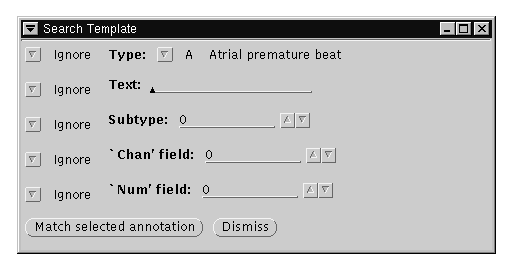
\epsfig{file=search-template.ps}}
\caption{The {\sf Search Template} window.}
\label{fig:search-template}
\end{figure}

In the {\sf Search Template}, you may select any combination of
annotation fields as search criteria using the abbreviated menu buttons to
the left of each field.  Enter the values to be matched next to each
active match control.  Any fields marked by `{\sf Ignore}' are not
used as match criteria.  In figure~\ref{fig:search-template}, the {\sf
Type}, {\sf Subtype}, and {\sf `Chan' field} criteria must be
satisfied by an annotation in order for \WAVE{} to consider that
annotation as a match;  the {\sf Text} and {\sf `Num' field} criteria
are ignored by \WAVE{}.

If the {\sf Text} criterion is active, \WAVE{} requires that the
specified text string appear in the {\tt aux} field of any matching
annotation.  Note that, as for search criteria specified in the {\sf
Search for} field of the {\sf Find} window, the {\tt aux} field of a
matching annotation is required only to \emph{contain} a matching text
string, and additional text may appear in the {\tt aux} field before
or after the matching string.

As a shortcut, click on \button{Match selected
annotation} to copy all fields of the selected annotation into the
{\sf Search Template}.  This action also sets all of the criteria menu
buttons to {\sf Match}.


\section{Saving your work}

In a lengthy editing session, \WAVE{} saves your annotation file periodically.
\index{annotation file!checkpointing}
\begin{wrapfigure}[9]{r}{2.2cm}
\mbox{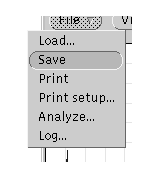
\epsfig{file=file-save.ps}}
\end{wrapfigure}
You can force \WAVE{} to save your edits
\index{saving edits}
at any time by selecting the {\sf Save} entry from
the {\sf File} menu.  Once all of the changes have been saved, \WAVE{}
removes the parentheses from the title bar.

\index{saving edits}
When you are finished, exit from \WAVE{} as in the first exercise.  It is
not necessary to take any explicit action to save your edits, since \WAVE{}
does so automatically on any normal exit (via \button{Quit}
\index{Quit button@{\sf Quit} button}
on the main control panel,
\marginpar{\emph{Do not use {\sf Quit} on the window menu to exit from
\WAVE{} 5.x and earlier;  these versions will not save your edits
before exiting this way.}}
or from the window menu).  You will find two new files in the
current directory.  The file called `{\tt qrs.100s}' is the edited version of
the annotation file that you have just created, and `{\tt \_qrs.100s}' is the
\index{backup}\index{annotation file!backup}
previous version (in this case, containing the unedited annotations as produced
by {\tt sqrs}).  At most one previous version is saved as a backup; if the
original annotation file is not located in the current directory (i.e., if it
was found elsewhere in the database path),
\index{database path}
it is left unchanged and \WAVE{} does not create a separate backup file.

\section{Creating an annotation file manually}

\index{annotation file!creating!manually}
\index{creating an annotation file!manually}
In this exercise, we created the annotation file using {\tt sqrs}, and then
edited it.  It is also possible to create an annotation file manually;  to
do so, simply fill in the {\sf Annotator} field
\index{Annotator@{\sf Annotator}}
in the {\sf Load} window
\index{Load window@{\sf Load} window}
\index{annotator name}
with the annotator name of your choice.  If there is no existing annotation
file associated with the specified annotator for the current record, \WAVE{}
creates an initially empty annotation file, to which you can add and edit
annotations just as we did in this exercise.

\section{Multi-edit mode}

\label{sec:multi-edit}
\begin{htmlonly}
\index{multi-edit mode}
\end{htmlonly}
\begin{latexonly}
\index{multi-edit mode|textit}
\end{latexonly}
\index{annotation!attached to signal}
\index{signal!annotating independently}
\marginpar{\emph{\WAVE{} 5.0 does not support the features described in this
section.}}
If you plan to use \WAVE{} with records containing signals that must be
annotated independently, read this section.

Using the \amenubutton{Show annotations} menu button
\index{View window@{\sf View} window}
in \WAVE{}'s {\sf View} window, you
\begin{wrapfigure}[6]{l}{6cm}
\mbox{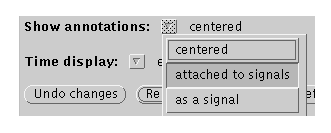
\epsfig{file=attach-to-signals.ps}}
\end{wrapfigure}
may choose to display annotations attached to signals, rather than
in the center of the signal window as is the usual default.  In this case, the
\index{chan in annotation@{\tt chan} in annotation}
\index{annotation!chan@{\tt chan}}
\index{signal!number}
{\tt chan} field of each annotation specifies the signal number of the signal
to which it is attached.  If annotation editing is enabled when annotations
are displayed in this way, \WAVE{} is in \emph{multi-edit mode}.

\index{signal!suppressing display}
\index{signal!list}
\WAVE{} draws the signals in order of signal number from the top to
the bottom of the signal window, beginning with signal number 0 at the
top of the signal window.  When annotations are attached to signals,
\WAVE{} draws them about 2 mm above the center of the range of the
attached signal (except for special annotations that are displaced
above or below the usual level).  Although this presentation usually
helps to avoid the visual confusion that might result from drawing
annotations directly on the associated signals, it may contribute to
confusion if the spacing between signals is too small (as may happen
if the signal window is reduced in height, or if many signals are
displayed).  If this becomes a problem, try increasing the height of
the signal window (by dragging on the resize handles on the window
frame), or displaying only a subset of the signals (by specifying
which signals are to be shown in the {\sf Signal list} field in \WAVE{}'s
{\sf Analyze} window, and selecting `{\sf listed signals only}' from the
\amenubutton{Draw:} menu in WAVE's {\sf View} window).

In multi-edit mode, annotation editing operations are slightly
different from those described above.  The most important difference
is that you must always point to the desired signal when inserting or
moving annotations.  In this mode, the {\tt chan} field in the {\sf Annotation
Template} window does not determine the {\tt chan} field of an inserted
annotation; rather, the signal to which you point determines the
{\tt chan} field, and the {\tt chan} field in the {\sf Annotation Template}
window is updated accordingly after each insertion.  To move an annotation to
a different signal, simply select it and drag the pointer to the
desired time and signal.  If you wish to change the {\tt chan} field of an
annotation without changing its time, select the annotation and use
the \keycap{$\uparrow$} and \keycap{$\downarrow$} keys to move it to the
desired signal.  Hold down \keycap{Ctrl} during these operations to copy the
annotation, rather than to move it (simultaneous annotations are
permitted if their {\tt chan} fields differ).

\section{About link annotations}
\label{sec:link-annotations}

\index{link annotation}\index{annotation!link}
A link (`{\tt @}') annotation permits external data to be associated
with a specific time (and, optionally, a specific signal) in a record.
\marginpar{\emph{The features described in this section are not supported by
\WAVE{} 5.0.}}
To make link annotations visually distinctive, WAVE{} displays them in
the color used for signals rather than that used for other
annotations, and it underlines them.  The {\tt aux} field of a link
annotation contains a URL (uniform resource locator) that points to
the external data, and an optional description displayed by \WAVE{} at
the location of the annotation.  (If the description is missing,
\WAVE{} displays the URL name.)

To view the external data associated with a link annotation, select it
and then press \keycap{Return} (or \keycap{Enter}).  \WAVE{} then
directs your web browser to display the data specified by the URL.
(If your web browser is not running, \WAVE{} starts it.)  By default,
\WAVE{} uses Netscape 1.1 or any later version available on the
\WAVE{} host.  To configure \WAVE{} to use a different browser, see
\hyperref{\WAVE{} and the Web}
{section~}
{, page~\pageref{sec:web}}
{sec:web}.

If the URL string does not contain a {\it protocol}{\tt ://} prefix
(where {\it protocol} is typically {\tt http} or {\tt ftp}), \WAVE{}
assumes that the URL refers to a file located somewhere in your WFDB
path.  In this case, \WAVE{} finds the file if possible, and attaches
the necessary path information to the beginning of the URL before
directing your web browser to display the associated data.

\WAVE{} does not include built-in facilities for editing external data.
You may insert and edit link annotations themselves, however, using
the normal annotation editing facilities of \WAVE{}.  To create a link
annotation, select `{\tt @}' from the {\sf Type} menu of the {\sf
Annotation Template}, and enter the URL in the {\sf aux} field.  If
you wish to supply a description to be displayed by \WAVE{} in place of
the URL, enter it after the URL, separating it from the URL with a
space character.  The current URL (i.e., the one associated with the
most recently selected link annotation) can be passed by \WAVE{} to an external
program such as a web browser or an HTML editor via the {\tt \$URL}
menu variable (see the comments in \WAVE{}'s menu file for details).

\section{Creating and using new annotation types}

\label{sec:creating-annotation-types}
\index{ANNTAB environment variable}\index{environment variables!ANNTAB}
\index{X11 resources!{\tt Wave.Anntab}}
\index{defining annotation types}\index{Type menu@{\sf Type} menu}
\index{annotation!table of definitions}
\WAVE{} was originally
developed for use with ECGs, and the standard set of annotation types
reflects this history.  If you work with other types of signals, or if
the standard set of annotations does not meet your needs, you may
define your own annotation types and add them to the
\amenubutton{Type:} menu in the {\sf Annotation Template}.  To do so,
first create a text file containing one-line entries defining each
new type, as described in
\hyperref{X11 Resources}
{section~}
{, page~\pageref{anntab},}
{sec:resources}
or see the file `{\tt anntab}' included
in the \WAVE{} distribution for an example.  Next, set the environment
variable {\tt ANNTAB}, or the X11 resource {\tt Wave.Anntab}, to the
name of this file.  The next time you run \WAVE{}, the new types from
your {\tt ANNTAB} file will appear in the \amenubutton{Type:} menu.
You may use them in the same way as the standard annotation types.
Any annotation files you create or edit while your {\tt ANNTAB} file
is loaded will contain embedded copies of your type definitions, so
that these files can be used on other systems and by other users
without the need to reference your {\tt ANNTAB} file each time.

\index{annotation!type codes}
\index{unassigned annotation type codes}
In most cases, you should use the unassigned type codes between 42 and 49 for
custom annotation types, rather than redefining the standard types.  If you
are not working with ECGs, however, you may redefine any type codes you wish
(the legal range is defined in `{\tt <wfdb/ecgcodes.h>'}).

\chapter{Analyzing Data with \WAVE{}}

For many users, \WAVE{}'s data analysis capabilities will be of
greatest interest.  \WAVE{} itself does not perform analysis of the
signals or annotations it displays.  What \WAVE{} offers is an
easy-to-use means of controlling external analysis programs and
viewing their outputs.  The buttons in the {\sf Analyze} window activate
these external programs.  These buttons are easy to create -- in fact,
you can add your own buttons to those in the {\sf Analyze} window
while \WAVE{} is running.

In the previous chapter, we used the \button{Mark QRS complexes}
button to run the standard WFDB application program {\tt sqrs}.  In this
chapter, we will see how \WAVE{} controls {\tt sqrs}, and we will create
and test a new button to generate a heart rate signal using {\tt sqrs}
and another standard WFDB application, {\tt tach}.  Discussions of
\WAVE{}'s ``logbook'' and ``oscilloscope'' facilities follow, and then
we study an extended example of how to develop an analysis program
controlled by \WAVE{}, using the C programming language.  At the end of
this chapter, we explore how this relationship can be inverted, so
that \WAVE{} can be driven by an external program.

As before, use \WAVE{} to open record {\tt 100s}:
\begin{verbatim}
    wave -r 100s
\end{verbatim}
Click right on \menubutton{File}, click left on
{\sf Analyze...}, and once again, click left on \button{Mark QRS complexes}.
\index{analysis commands window@{\sf Analysis Commands} window}
Where does the command that appears in the {\sf Analysis Commands} window,
\begin{verbatim}
    sqrs -r 100s -f 0 -t 1:00.000 -s 0
\end{verbatim}
come from, and what does it mean?

\index{sqrs command@{\tt sqrs} command}
If you refer to the {\tt man} page for {\tt
sqrs},
\htmladdnormallink{{\tt sqrs(1)}}{../dbag/sqrs-1.htm}
(either by typing `{\tt man sqrs}' in a terminal emulator window, or by
looking it up in the
\htmladdnormallink{{\it WFDB Applications Guide}}{../dbag/dbag.htm}),
you will see that
the second command-line argument ({\tt 100s}) is (not surprisingly) the record
name, `{\tt -f 0}' instructs {\tt sqrs} to start at the beginning of the
record, `{\tt -t 1:00.000}' tells it to stop 1 minute later, and `{\tt -s 0}'
specifies that signal 0 is to be used for QRS detection.

\section{\WAVE{}'s menu file}

\label{sec:menu-file}
\index{menu file}
To understand where the command comes from, we need to inspect \WAVE{}'s
\begin{wrapfigure}[12]{r}{7.25cm}
\mbox{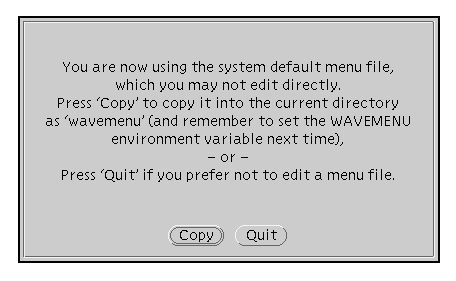
\epsfig{file=system-menu.ps}}
\end{wrapfigure}
\emph{menu file}. Click left on the \button{Edit menu} button in the
{\sf Analyze} window. Unless your
\WAVE{} menu has already been customized, \WAVE{} pops up a
notice as shown at right.
Click left on \button{Copy} to continue with this exercise.  After a few
seconds, the \WAVE{} menu file appears (in an OpenWindows {\tt textedit}
window as in figure~\ref{fig:wave-menu}, unless you have specified a
different editor by setting the {\tt EDITOR} environment variable).
\index{EDITOR environment variable}
\index{environment variables!EDITOR}
\index{textedit command@{\tt textedit} command}

\begin{figure}
\centerline{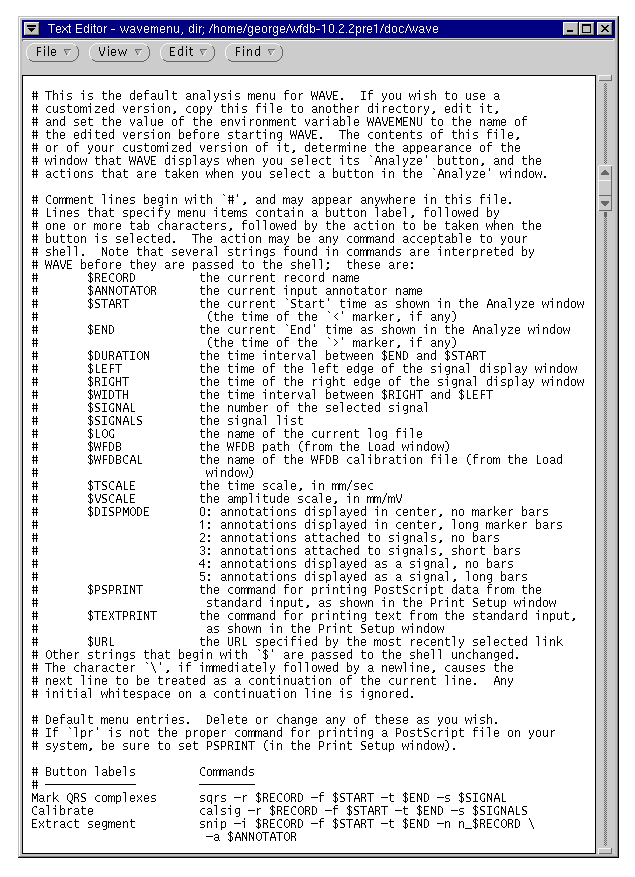
\epsfig{file=wave-menu.ps}}
\caption[\WAVE{}'s menu file]{The beginning of \WAVE{}'s menu file, in
a {\tt textedit} window.}
\label{fig:wave-menu}
\end{figure}

\index{Analyze window@{\sf Analyze} window}
\index{analysis commands window@{\sf Analysis Commands} window}
\index{menu variables}
The comments at the beginning of the \WAVE{} menu file describe how it
works.  Each of the buttons in the {\sf Analyze} window (except for
those in the first three rows) corresponds to an entry in the menu
file.  The first part of the entry -- up to the first tab character --
specifies the label that appears on the button; the remainder of the
entry specifies the command that is inserted into the {\sf Analysis
Commands} window if you click left on the button.  As noted in the
comments, certain strings that begin with `{\tt \$}' are recognized as
\index{menu variables}\index{variables!in \WAVE{} menu file}
\emph{menu variables} and are interpreted by \WAVE{} before being
passed to the shell in the {\sf Analysis Commands} window.  In the
case of the {\tt sqrs} command that appears in the {\sf Mark QRS
complexes} entry, these strings are `{\tt \$RECORD}', `{\tt \$START}',
`{\tt \$END}', and `{\tt \$SIGNAL}'.  \WAVE{} replaces `{\tt
\$RECORD}' with the record name, as it appears in the {\tt Record}
field of the {\sf Load} window.  `{\tt \$START}' is the time of the
`{\tt <}' marker, shown in the {\sf Start} field of the {\sf Analyze}
window; if no `{\tt <}' marker has been defined, the {\sf Start} field
contains the string `{\sf beginning of record}', and `{\tt \$START}'
becomes {\tt 0}.  Similarly, `{\tt \$END}' is the time of the `{\tt
>}' marker, shown in the {\sf End} field; if no `{\tt >}' marker has
been defined, the {\sf End} field is `{\sf end of record}', and `{\tt
\$END}' is determined by the record length as encoded in the header
file for the record (see
\htmladdnormallink{{\tt header(5)}}{../dbag/header-5.htm},
in the
\htmladdnormallink{{\it WFDB Applications Guide}}{../dbag/dbag.htm}).
Finally, `{\tt \$SIGNAL}' is taken from the
{\sf Signal} field of the {\sf Analyze} window; it specifies which
signal is to be analyzed.
\marginpar{\emph{The signal list does not exist in \WAVE{} 5.0.}}
(For applications that can analyze more than one signal,
the string `{\tt \$SIGNALS}' is taken from the {\sf Signal list}
\index{signal!list}
field.)  Examine the commands defined in the default \WAVE{} menu;
they should give you an idea of what is possible.

\section{Defining a region of interest}

\index{region of interest}
\index{marker!{\tt >}}
\index{marker!{\tt <}}
A common problem in many cases is simply selecting a segment to be analyzed,
from a digitized signal file that may include extraneous material at the
beginning or at the end.  As you can see from the {\tt sqrs} example, this can
be done easily by inspecting the signals with \WAVE{} and placing `{\tt <}'
and `{\tt >}' markers at the beginning and end of the region of interest.  If
the analysis program is written to accept starting and ending times (more on
this subject below), these times can be passed as command-line arguments by
\WAVE{}.  Similarly, it's simple to choose one or more of a number of
signals to analyze after viewing them with \WAVE{} (either type into the
{\sf Signal} field directly, use the increment/decrement buttons, or
\marginpar{\emph{\WAVE{} 5.0 does not support `point-and-click' signal selection.}}
point to a
signal in the signal window, press and hold the \keycap{Shift} key, and click
left).  Close the {\tt textedit} window and experiment with changing the {\sf
Start}, {\sf End}, and {\sf Signal} fields of the {\sf Analyze} window, and
running {\tt sqrs}, until you are familiar with the results.

\section{Analysis example: Generating a heart rate signal}
In the rest of this exercise, we'll develop a command for generating a heart
rate signal, add it to the \WAVE{} menu, and test it.  First, set the {\sf
Start} and {\sf End} fields to {\tt 0} and {\tt 1:0} respectively, and click on
\button{Mark QRS complexes} to regenerate the annotation file.  Open
the annotation file using the {\sf Load} window.

\index{WFDB Software Package}
\index{tach command@{\tt tach} command}
Generating a heart rate signal is simple enough, given a beat annotation file
and 
\htmladdnormallink{{\tt tach}}{../dbag/tach-1.htm},
a program supplied as part of the WFDB Software Package.  {\tt
tach} reads an annotation file, calculates an instantaneous heart rate for each
cardiac cycle from the reciprocal of the interval between successive beat
annotations, and then uniformily resamples this signal (by default, at 2 Hz).
Referring to the 
\htmladdnormallink{{\it WFDB Applications Guide}}{../dbag/dbag.htm},
we find the command we need to generate a heart rate signal from
`{\tt qrs.100s'}:
\begin{verbatim}
    tach -r 100s -a qrs -f 0 -t 1:0
\end{verbatim}

\index{analysis commands window@{\sf Analysis Commands} window}
If this command is typed into the {\sf Analysis Commands} window, it prints:
\begin{verbatim}
    73.9726
    73.9726
    73.7238
       .
       .
       .
    75.7788
    74.5703
    73.8015
\end{verbatim}
These numbers are the calculated samples of the heart rate signal (the units
are beats per minute).

We can generalize this command as:
\begin{verbatim}
    tach -r $RECORD -a $ANNOTATOR -f $START -t $END
\end{verbatim}
where the parameters {\tt \$RECORD}, {\tt \$ANNOTATOR}, etc., are replaced by
the appropriate values when the command is executed.  This is the form of the
command we should add to \WAVE{}'s menu;  by parameterizing the arguments
in this way, we can use \WAVE{} to select a record, annotator, and segment
to be analyzed as for the other commands in the menu.  To add this command
to the menu, click on \button{Edit menu} again.  Position the cursor at the end
of the menu file and add the line:
\begin{verbatim}
   Heart rate<TAB>tach -r $RECORD -a $ANNOTATOR -f $START -t $END
\end{verbatim}
where {\tt <TAB>} represents one or more {\sf TAB} characters; at least one
{\sf TAB} must be present (spaces don't count).  Be sure to end the line with
{\sf RETURN}.  Save the menu (choose {\sf Save} from the {\tt
textedit} window's \menubutton{File} menu), and quit from {\tt textedit}.  Now
\index{textedit command@{\tt textedit} command}
click on \button{Reread menu} in the {\sf Analyze} window.  The {\sf Analyze}
window will disappear briefly, then reappear (possibly in a different location,
depending on your window manager) with a new \button{Heart rate} button.  If
you click on this button, \WAVE{} executes the {\tt tach} command as above.

You might prefer to look at heart rate as a signal rather than as a column of
numbers.  {\tt tach} has the capability of generating an output signal file
instead of text.  To try this out, edit the menu file again, and add `{\tt -o
hr\_\$RECORD}' to the end of the entry.  (You may split the command across two
lines using a `{$\tt \backslash$}' at the end of the first line if you wish.)
Once again, save the menu file, quit from {\tt textedit}, click on
\button{Reread menu}, and on \button{Heart rate}.  This time, there is no text
output from {\tt tach}; if you enter `{\tt hr\_100s}' in the {\sf Record}
field of the {\sf Load} window, however, \WAVE{} displays the calculated
heart rate signal.
\begin{figure}
\centerline{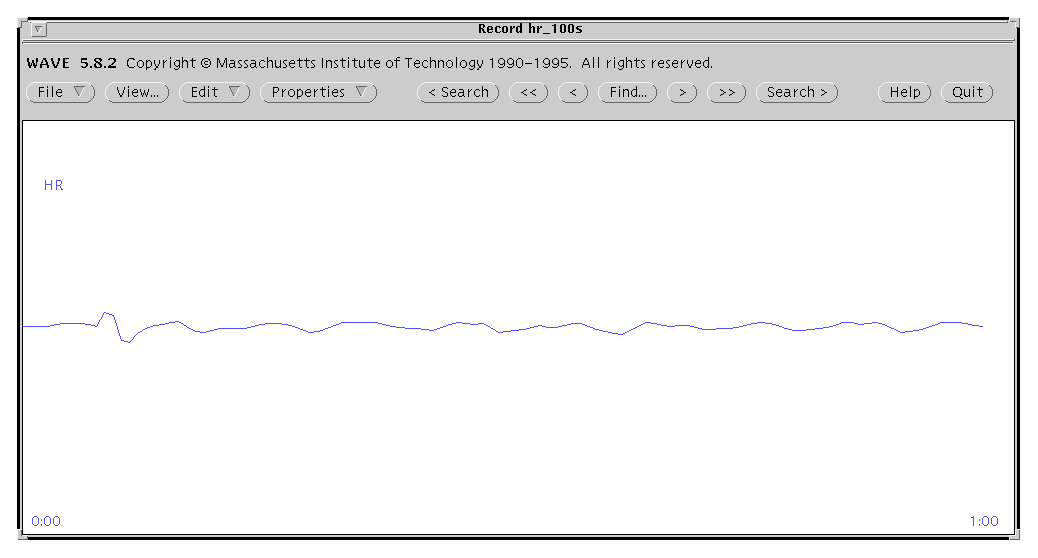
\epsfig{file=main-with-hr.ps}}
\caption{Heart rate signal.}
\label{fig:main-with-hr}
\end{figure}
\index{time scale}\index{amplitude scale}
\index{scales!setting}\index{display scale}
\index{View window@{\sf View} window}
(You may wish to change the time and amplitude scales using the {\sf View}
window, in order to see more of the signal at once.  If you set the
time scale to 250 mm/min and the amplitude scale to 100 mm/mV, you
will be able to see the heart rate signal for the entire record as in
figure~\ref{fig:main-with-hr}; the
periodic modulation is due to respiratory sinus arrhythmia.)

\section{The signal list}

\index{signal!list}
Although this exercise used only one signal of the input record, many
applications will use two or more signals simultaneously.  The {\sf Signal
list} initially contains the signal numbers of all available signals; as noted
\marginpar{\emph{These features are not available in \WAVE{} 5.0.}}
above, the signal list can be passed to an application listed in the menu file
as a set of command-line arguments in place of the string `{\tt \$SIGNALS}'.
Although you can type into the {\sf Signal list} field directly to change it,
you can also do so using the mouse.  Pointing to a signal, hold down the
\keycap{Control} key while clicking left to add it to the signal list, or hold
down the {\sf Meta} key while clicking left to delete its first
\index{Meta key@{\sf Meta} key}
occurrence from the signal list.  (Most keyboards do not have a key
labelled {\sf Meta}.  On most Sun keyboards, the {\sf Meta} keys look like
this: \keycap{$\Diamond$};  they flank the space bar.  On most
other keyboards, the \keycap{Alt} key is equivalent to {\sf Meta}.)

\section{Using a customized menu file}

\index{WAVEMENU environment variable}\index{environment variables!WAVEMENU}
\index{menu file}
\index{default menu}
Recall that when you first examined the menu file, \WAVE{}
warned you to set the {\tt WAVEMENU} variable the next time you run \WAVE{}.
{\tt WAVEMENU} should be set to the name of your customized menu file (you
can give the menu file any name you choose;  {\tt wavemenu} is the default
name).  For example, if you use the C-shell and {\tt wavemenu} is in your home
directory, use the command
\begin{verbatim}
    setenv WAVEMENU ~/wavemenu
\end{verbatim}
before running \WAVE{} again.  You may wish to add this command to your
\index{login@{\tt .login}}
{\tt .login} script to set the variable automatically each time you log in.
\marginpar{\emph{\WAVE{} 5.0 always uses the system default if {\tt
WAVEMENU} is not set.}}
(If you forget to set {\tt WAVEMENU}, \WAVE{} will find your customized menu
file only if it is in the current directory and is named {\tt wavemenu};
otherwise, \WAVE{} will use the system default menu again.)

\section{Using the {\sf Log} window}

When examining a recording, you may find features that you wish to
document for further study.  In addition to its capabilities for
interactive annotation editing, \WAVE{} also offers an easy-to-use
``logbook'' for collecting brief notes about segments to which you
may wish to return.  Each entry in a \WAVE{} log file contains the
record name, time, and an optional comment -- so it is possible to
put together a collection of examples taken from any number of records
in a single log.  Once the log has been created, the entries in it can be
reviewed very easily, or the log can be used as a script for {\tt
pschart}, which will print the signals, annotations, and your comments
for each entry, changing records automatically.

Open the {\sf Log} window (see figure~\ref{fig:log-window}) by choosing
{\sf Log...} from \WAVE{}'s \menubutton{File} menu.
\begin{figure}
\begin{htmlonly}
\index{Log window@{\sf Log} window}
\end{htmlonly}
\begin{latexonly}
\index{Log window@{\sf Log} window|emph}
\end{latexonly}
\centerline{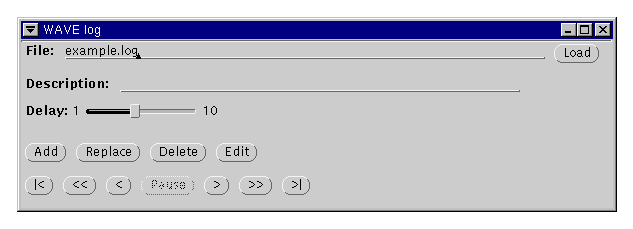
\epsfig{file=log-window.ps}}
\caption{The {\sf Log} window.}
\label{fig:log-window}
\end{figure}
When you first open the {\sf Log} window, many of its controls are
dimmed until you specify a log file and begin adding entries to it.
To create a log file, or to review or add to an existing one, enter
its name in the {\sf File:} field of the {\sf Log} window.

To add an entry, use \WAVE{}'s navigation controls so that the segment
upon which you wish to comment appears in the signal window.  Enter
your comments in the {\sf Description:} field, then click on \button{Add}.

The log navigation buttons become visible once there are log entries
recorded.  You can use \button{\tt <} and \button{\tt >} to step
through the log one entry at a time, or use \button{\tt <<} or
\button{\tt >>} to present a ``slide show'' (control the length of
time each entry appears using the {\sf Delay:} slider, and use
\button{Pause} to interrupt the show).  \button{\tt |<} and
\button{\tt >|} can be used to jump directly to the beginning or the
end of the log.

To replace a log entry, first use the log navigation buttons to
display that entry.  Make any adjustments necessary (use the
navigation buttons in \WAVE{}'s main window to reposition the signal
window as needed, and correct the log entry text in the {\sf
Description:} field), then click on \button{Replace}.

To delete a log entry, select it first as above, then click on
\button{Delete}.  For more complex editing (such as rearranging
entries), click on \button{Edit} to open the log file in a {\tt
textedit} window (or in the editor of your choice, if you have
set the {\tt EDITOR} environment variable).  After completing your
edits, save them and exit from the editor, then click on \button{Load}
to reload the edited log into \WAVE{}.  (You can also use \button{Load}
if another process, such as one started from the {\sf Analyze} window,
has modified the log file.)

\label{sec:printing-log}
\index{printing!log with charts}
\index{log!printing with charts}
\WAVE{}'s default menu file contains a commented-out entry with the tag
\marginpar{\emph{This function does not exist in \WAVE{} 5.0.}}
``Print log with charts''.  If a button with this text does not appear
in the {\sf Analyze} window, click on \button{Edit menu}, remove the
comment characters from this entry, save the menu and exit the editor,
and click on \button{Reread menu}.  You can now print the log together
with the signals and annotations by clicking on \button{Print log with
charts}.

\newpage
\section{Using the {\sf Scope} window}

\index{Scope window@{\sf Scope} window}
\begin{wrapfigure}{l}{2cm}
\mbox{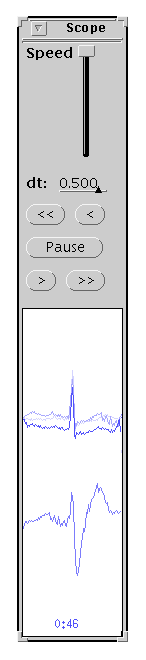
\epsfig{file=scope-window.ps}}
\caption[The {\sf Scope} window.]{\sf Scope}
\end{wrapfigure}
Some types of signals are characterized by changes in waveform shape
(morphology), which may occur gradually or suddenly.  For example,
ischemic ST changes in the ECG are usually visible as quasi-continuous
changes over a period of at least 30 seconds (often much longer).  It
can be helpful to view such signals on an oscilloscope, where the
trigger can be adjusted so that the (approximately) periodic waveforms
are superimposed.  Such displays, and their digital counterparts, are
very widely used in analysis of long-term ECG recordings.  \WAVE{}'s
{\sf Scope} window offers some of the features of this type of
display, with a few unique capabilities and limitations of its own.

To open the {\sf Scope} window, first open the {\sf Analyze} window,
then click left on \button{Show scope window}.
The {\sf Scope} window simulates an oscilloscope by using color map
animation (on hardware with an X server that supports this technique)
or stipple masks (otherwise).  The display is ``triggered'' by beat
(QRS) annotations (other annotations, such as rhythm changes, are
ignored).  As each waveform is drawn, the previously drawn waveform is
made to fade progressively into the background, disappearing
completely after four new waveforms have been drawn.  The appearance
is similar to that of an analog scope with moderately long-persistence
phosphor.  The x-position in the window of the trigger point (the
sample that the annotation points to for each waveform) is adjustable
using the {\sf dt:} setting (the value is expressed in seconds, and
may be negative).  It is also possible to resize the window, so that
several waveforms can be viewed side-by-side as well as superimposed.
As shown in the figure at left, \WAVE{} shifts waveforms to the bottom
of the window if they have been annotated as ventricular ectopic
beats.  (This behavior was chosen to be most useful for studying ECGs,
but other signals can be annotated in the same way if desired.)

The navigation controls are similar to those in the {\sf Log} window.
\button{\tt <} and \button{\tt >} may be used to move backward and
forward through the record one beat at a time.  \button{\tt <<} and
\button{\tt >>} provide a continuous ``movie'' (at a speed controlled
by the {\sf Speed} slider) that can be interrupted by \button{Pause},
which also recenters the signal window on the current beat.  Whenever
the current beat is visible in the signal window, it is marked with
the selection rectangle.

\index{signal!selecting}
Only one signal at a time can be displayed in the {\sf Scope} window.
Select that signal using the {\sf Signal} field in the {\sf Analyze}
window, or press and hold the \keycap{Shift} key while clicking left
in the signal window near the desired signal.

\section{Analysis example: Measuring ST deviations}

We now turn to an extended example showing how an
application can be written in C to be used with \WAVE{}.  The
application is an example only;  it is not intended for any serious
application, clinical or otherwise.  Its structure illustrates,
however, how a real application can be built.

As noted in the previous section, changes in the ST segment of the ECG
are of interest because of their relationship to ischemia
(which occurs when the oxygen supplied by the coronary arteries is
insufficient to meet the demands of the myocardium).
Characteristically, ischemia affects the shape of the ST segment, 
which corresponds to the first phase of ventricular repolarization
following the QRS complex;  typically, the ECG signal may not return 
to its baseline, or isoelectric, level (defined in the interval
between the P-wave and the QRS complex) until after the T-wave.  The
level of the ST segment relative to the isoelectric level is the ST
deviation.  Conventionally, the ST deviation is measured at a single
point 80 milliseconds after the J point (the end of the QRS complex).
An ST deviation of 100 $\mu$V is considered to be clinically
significant, and consistent with ischemia.

We will design a program for measuring ST deviations using \WAVE{}.  We
assume that the QRS complexes have been marked, and that, in addition,
two special annotations (`{\tt (}', signifying the beginning of the QRS
complex, and `{\tt )}', signifying its end) have also been marked for the
first beat that we wish to measure.  (To use our program on an
unannotated record, we can use \button{Mark QRS complexes}, and then
insert the special annotations manually around the first beat.)

Let us begin by deciding how the program should be invoked from \WAVE{}.
At a minimum, we should be able to specify which signal should be
measured, and the region of interest.  The program also needs to know
\index{record!name}
\index{annotator name}
the record and annotator names (the latter so that it can read the
annotations it needs to get started).  Following the conventions
used by many other WFDB applications, we add the following entry to
\WAVE{}'s menu file:

\begin{verbatim}
Measure ST deviation<TAB>stdev -r $RECORD -a $ANNOTATOR \
                          -f $START -t $END -s $SIGNAL
\end{verbatim}
%$
\htmladdnormallink{Here}{stdev.c}
is the C source for the program.  If this looks unfamiliar, read
about how to write WFDB applications in the
\htmladdnormallink{{\it WFDB Programmer's Guide}}{../dbpg/dbpg.htm}.

\begin{latexonly}
{\small
\verbatiminput{stdev.c}
}
\end{latexonly}

The source for this program is included in the \WAVE{} distribution as
{\tt stdev.c}.  Copy this file to the \WAVE{} host if necessary, and
compile it in a terminal window using a command such as
\begin{verbatim}
    cc -o stdev -O stdev.c -lwfdb
\end{verbatim}
Depending on how the WFDB Software Package has been installed on the
\WAVE{} host, you may need to use {\tt -I/usr/local/include} and
{\tt -L/usr/local/lib} options so that the compiler can
locate the {\tt *.h} files and the WFDB library.  On some systems, the
C compiler may have a different name, such as {\tt gcc}.  Consult an
expert such as your system administrator if in doubt about compiling
a C program with the WFDB library.

Once the source has been compiled successfully, install the executable
binary file {\tt stdev} in a directory in your {\tt PATH}.  If you
are using the C-shell, you may need to run the command {\tt rehash} to
make your shell aware that the program has been installed.  Test the
program in the terminal window by typing

{\tt stdev}

\noindent
which should produce a brief summary of its options.   \emph{If this
test fails, figure out why and correct the problem before continuing.}

Once the program has been compiled and installed successfully, try
running it from within \WAVE{}.  Remember that the annotation file must
include the `{\tt (}' and `{\tt )}' annotations to mark the beginning
and end of the first beat to be measured.  Using it on signal 0 of
record 100s, with a suitably augmented set of reference annotations, I
obtained output beginning with:
\begin{verbatim}
    0.0171296	-84
    0.0306481	-24
    0.0437963	-9
    0.0569907	-34
    0.0701389	-64
    0.08375	-59
    0.0946296	-49
    0.111204	-29
    0.125278	-4
    0.138796	-59
    0.151944	-9
    0.164815	-34
\end{verbatim}

(Your output will vary, depending on the exact locations of the
`{\tt (}' and `{\tt )}' annotations that you insert.)

\index{plot2d command@{\tt plot2d} command}
You can plot this output by piping it to the {\tt plot2d} command (see
\marginpar{\emph{{\tt plot2d} will not work unless {\tt gnuplot} has
been installed.  {\tt gnuplot} is included in most Linux distributions,
and is also available by anonymous FTP from
\htmladdnormallink{{\tt prep.ai.mit.edu}}{ftp://prep.ai.mit.edu} and
numerous other sites.  If {\tt plt} is available on your system, you may use
it instead of {\tt plot2d} (with the same options).}}
\htmladdnormallink{{\tt plot2d(1)}}{../dbag/plot2d-1.htm}, in the
\htmladdnormallink{{\it WFDB Applications Guide}}{../dbag/dbag.htm},
for details on {\tt plot2d}, a command-line preprocessor for {\tt
gnuplot}).
To do so, modify the entry in the menu file, so that it becomes:
\begin{verbatim}
    Plot ST deviation<TAB>stdev -r $RECORD -a $ANNOTATOR \
                            -f $START -t $END -s $SIGNAL | \
                           plot2d 0 1 \
                            -t "ST deviations, Record $RECORD" \
                            -x "Elapsed time (minutes)" \
                            -y "ST deviation (microvolts)"
\end{verbatim}

If you now reread the menu and use the new \button{Plot ST deviation}
button, {\tt plot2d} opens a window with a plot in it, similar to
figure~\ref{fig:stdev-plot}.
\begin{figure}
\centerline{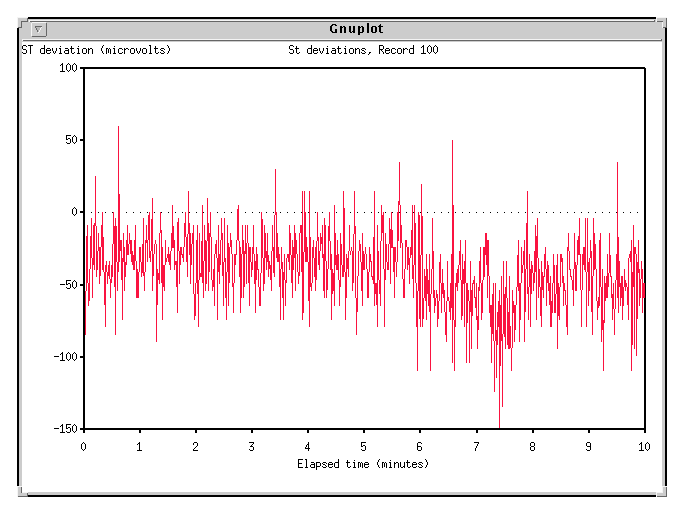
\epsfig{file=stdev.ps}}
\caption{ST deviations measured by the example program.}
\label{fig:stdev-plot}
\end{figure}
(To make this plot, I used the first ten minutes of record 100; the
sample record 100s contains only the first minute of data shown in the
plot.)  This window stays open until you dismiss it by pressing
\index{analysis commands window@{\sf Analysis Commands} window}
\keycap{Enter} (\keycap{Return}) in the {\sf Analysis Commands}
window; if you forget to do so, the next command you run from the {\sf
Analyze} window will serve this function (but the command itself won't
run, since {\tt plot2d}, rather than the command interpreter, will
have read the command string).

\subsection*{Further work}
If you would like to make this program work better, here are a few
ideas:

\begin{itemize}
\item
Extending it to make measurements on multiple signals is an easy project.
Allow the user to set measurement reference points on each signal separately.

\item
It's also not too difficult to copy the input annotation file, writing
the measurements into the {\tt num} fields of the annotations, so that
\WAVE{} can display them as a signal.  If you try this, keep in mind
that {\tt num} values must be integers in the -128 to 127 range, so
don't record the deviations in $\mu$V.  If you want to write the
measurements into a \emph{signal} file (as we did with {\tt tach}
earlier in this chapter), this can get complicated---see the source
for {\tt tach} for hints about doing this.

\item
The measurement point should move closer to the J point at high heart rates;
see any reference on the ECG for a discussion of this issue.

\item
The measurements as made above are very easily contaminated by small amounts
of noise in the signals.  You should be able to improve them significantly by
averaging the amplitudes of several samples in the neighborhoods of
the isoelectric point and the ST level measurement point.

\item
The program should not produce measurements for ventricular ectopic beats,
or for beats that are extremely noisy.  Noise detection is an
interesting research problem in itself.

\item
You may wish to examine using beat averaging (or median filtering) to reduce
noise in the measurements further; the
\htmladdnormallink{{\it WFDB Programmer's Guide}}{../dbpg/dbpg.htm}
describes a beat averager that may be a useful starting point.

\item
Another source of measurement error is baseline wander in the ECG,
visible as slopes in the intervals between beats.  You can reduce this
error by \emph{modelling} the baseline drift and subtracting it from
the signal.  Simple linear models, or quadratic or cubic splines, can
be used.
\end{itemize}

\section{Controlling \WAVE{} from an external program}
\label{sec:wave-remote}

Although the facilities discussed in the previous sections provide
highly flexible control of external analysis programs, in some cases
it is desirable for another program to control \WAVE{} rather than for
that program to run under \WAVE{}'s control.

The program {\tt wave-remote}, provided with the \WAVE{} distribution,
can drive
\marginpar{\emph{{\tt wave-remote} is not provided with \WAVE{} 5.0,
which does not allow for external control.}}
\WAVE{}'s display.  Using {\tt wave-remote}, you can cause
\WAVE{} to go to any specified location in the current record, to load
another set of annotations for the current record, or to open another
record.  By providing a command-line interface for driving \WAVE{}, {\tt
wave-remote} simplifies the task of driving \WAVE{} from other programs
or shell scripts; in general, it is sufficient merely to fork a new
process and invoke {\tt wave-remote} with the appropriate arguments
(for example, using the {\tt system()} function provided in the
standard C library).  If it is not acceptable to start a new process
for this purpose, {\tt wave-remote} is also provided in C source form,
and the functions it uses to drive \WAVE{} can be invoked directly from
your program.

Options for {\tt wave-remote} are:

\begin{description}
\item[{\tt -pid} \textit{processid}]
Control the \WAVE{} process with the specified \textit{processid}.
(If this option is omitted, and more than one instance of \WAVE{} is
running, {\tt wave-remote} controls the one with the highest
\textit{processid}.)

\item[{\tt -r} \textit{record}]
(Re)open the specified \textit{record}.

\item[{\tt -a} \textit{annotator}]
(Re)open the specified \textit{annotator} for the current record.

\item[{\tt -f} \textit{time}]
Go to the specified \textit{time} in the current record.
\end{description}

For example, the command
\begin{verbatim}
    wave-remote -r 100s -a atr -f 0:22
\end{verbatim}
causes \WAVE{} to open record {\tt 100s}, with annotator {\tt atr},
and to show data starting at 22 seconds after the beginning of the record.

If \WAVE{} is not running when {\tt wave-remote} is invoked, {\tt
wave-remote} launches \WAVE{} provided that the record to be opened has been
specified.  Once {\tt wave-remote} has delivered its instructions to
\WAVE{}, it exits immediately.

As an alternative to the command-line interface offered by {\tt
wave-remote}, the {\tt wavescript} application provides the same
services, but is controlled by a script file (named on the {\tt
wavescript} command line).  Scripts for {\tt wavescript} should contain
on each non-comment line a single option/argument pair as described
above for {\tt wave-remote}.  Any line that does not begin with a
`{\tt -}' is treated as a comment line.  For example, if the file {\tt example.xws} contains
\begin{verbatim}
    # Here is a comment
    -r 100s
    -a atr
    -f 0:22
\end{verbatim}
then the command `{\tt wavescript example.xws}' has the same effect as
the {\tt wave-remote} example above.

Using these interfaces, an analysis program (or any program, such as a
web browser) can drive \WAVE{}'s display automatically.  In a typical
application, a semi-automated analysis program might require the user
to make or correct annotations for portions of a record that are
selected as part of the program's analysis (and that cannot be known
\emph{a priori}).

An analysis program that runs {\tt wave-remote} or {\tt wavescript}
may itself be running within \WAVE{}'s own {\sf Analysis Commands}
window.  This might be useful to permit the user to set the region of
interest interactively, before the analysis begins and takes over
control of \WAVE{} to show its progress or to obtain additional input.

\section{\WAVE{} and the Web}
\label{sec:web}

In this section we explore how World Wide Web documents and WFDB records
(i.e., signals and annotations viewable using \WAVE{}) can be linked
using \WAVE{} together with a web browser.  Beginning with \WAVE{}
6.0, it is possible while running a web browser to click on a link
from a web document to a specified location in a WFDB record and have
\WAVE{} open the record at that location.  It is similarly possible while
running \WAVE{} to click on a 
\hyperref{link annotation}
{link annotation (see section~}
{, page~\pageref{sec:link-annotations})}
{sec:link-annotations}
and have your web browser open the data specified by the link.

\subsection*{Controlling \WAVE{} from a web browser}

Most web browsers, such as Netscape, can use so-called \emph{helper}
or \emph{viewer} applications.  These are external applications that
are invoked by the browser to present data in formats that (usually)
are not supported by the browser directly.  For example, browsers
often use {\tt ghostscript} to display PostScript data.  It is
possible to configure Netscape and other web browsers so that \WAVE{}
can be used indirectly as a helper application.

By using
\hyperref{{\tt wavescript}}
{{\tt wavescript} (see section~}
{, page~\pageref{sec:wave-remote})}
{sec:wave-remote}
as the helper application for viewing WFDB records, an already-running
\WAVE{} process can be made to open a record and an annotation set and
to move to a specified location in the record.  With this approach, it
is not necessary to start a new \WAVE{} process each time.

You can set up your browser to view files with the MIME type
{\tt application/x-wavescript} or suffix {\tt .xws} using {\tt
wavescript}.  To do so, add the line
\begin{verbatim}
    type=application/x-wavescript  exts=xws
\end{verbatim}
to the file named {\tt .mime.types} in your home directory, and add the line
\begin{verbatim}
    application/x-wavescript; wavescript %s
\end{verbatim}
to the file named {\tt .mailcap} (also in your home directory).  If
your browser is Netscape, you can make these additions to {\tt
.mime.types} and {\tt .mailcap} by choosing {\sf General Preferences}
from the Options menu, clicking on the {\sf Helpers} tab, then
clicking on the {\sf New} button.  Fill in the dialog box as shown in
figure~\ref{fig:netscape-new-helper}, then save your settings.
\begin{figure}
\centerline{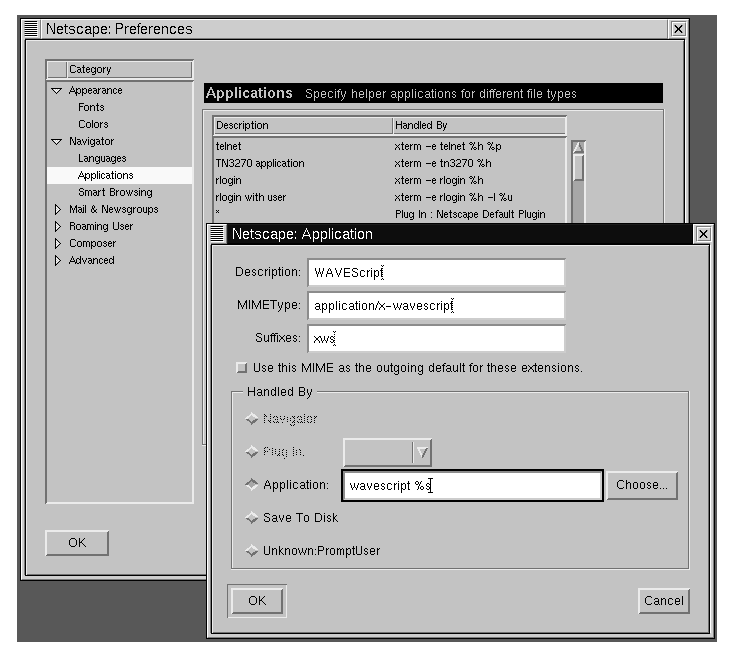
\epsfig{file=netscape-new-helper.ps}}
\caption{Adding {\tt wavescript} as a Netscape helper.}
\label{fig:netscape-new-helper}
\end{figure}

\begin{latexonly}
\begin{wrapfigure}[3]{l}{1.5cm}
\mbox{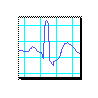
\epsfig{file=wave-icon.ps}}
\end{wrapfigure}
Once {\tt wavescript} has been installed as a helper application, your
web browser will launch {\tt wavescript} whenever you click on a link
to a {\tt .xws} script file.  As an example, 
the on-line version of this guide contains a link to the {\tt
example.xws} script shown in the previous section.  
\end{latexonly}
\begin{htmlonly}
Once {\tt wavescript} has been installed as a helper application, your
web browser will launch {\tt wavescript} whenever you click on a link
to a {\tt .xws} script file.  As an example, 
here is a link to the {\tt example.xws} script shown in the previous
section:
\end{htmlonly}
\begin{rawhtml}
   <a href="example.xws">
   <img src="wave.gif" alt="click here to view waveforms"></a>
\end{rawhtml}
To provide such a link in an HTML document, use a statement such as
\begin{verbatim}
   <a href="example.xws">
   <img src="wave.gif" alt="click here to view waveforms"></a>
\end{verbatim}
\begin{latexonly}
The {\tt wave.gif} icon (shown above) is provided in the \WAVE{}
distribution.
\end{latexonly}

\subsection*{Serving {\tt .xws} files}

If you plan to make {\tt .xws} files available from a Web server, you
will also need to configure your Web server so that it sends the
appropriate MIME type encoding ({\tt application/x-wavescript})
whenever a browser requests a {\tt .xws} file.  (When you use a
browser to read a local file, this is not required, since no Web
server is involved in this case; rather, the local {\tt .mime.types}
file is used by the browser to recognize the type based on the file
suffix.)

To configure the Apache {\tt httpd} (at this time, the most widely-used
Web server), find the file {\tt srm.conf} (typically in {\tt
/etc/httpd/conf}) and add the line
\begin{verbatim}
  AddType application/x-wavescript .xws
\end{verbatim}
in the section that contains other {\tt AddType} directives.  Restart
the server to force it to reread {\tt srm.conf}.  The NCSA {\tt httpd}
and variants of it can be configured in the same way;  if you use the
CERN {\tt httpd}, the configuration file is {\tt httpd.conf}, and the
syntax of the {\tt AddType} directive is different:
\begin{verbatim}
  AddType .xws application/x-wavescript text
\end{verbatim}
If you use some other Web server, consult its documentation to see how
to proceed.

Note that readers of Web pages with a link to a {\tt .xws} file will
need to have \WAVE{} and {\tt wavescript}, as well as the WFDB record
indicated in the {\tt .xws} file, available to them \emph{on the
system on which their Web browser is running}.

Note that if you attempt to read a {\tt .xws} file before completing
the necessary configuration steps, your browser's cache may interfere
with proper operation after the configuration is completed.  If this
happens, simply delete any {\tt .xws} files from your browser's cache.

\subsection*{Controlling a web browser from \WAVE{}}

\WAVE{} uses a web browser to display external data associated
with link annotations, and to display the on-line version of this
guide.  A suitable web browser must be installed on the \WAVE{} host
in order for this to work.  By default, \WAVE{} uses Netscape version
1.1 (or any later version;  free copies of Netscape for academic use
or for evaluation purposes may be obtained by anonymous FTP from
\htmladdnormallink{{\tt ftp.netscape.com}}{http://www.netscape.com}).

\WAVE{} controls the web browser in the same way it controls other
external programs:  by running commands in the {\sf Analysis Commands}
window.  \WAVE{}'s interface to the web browser is defined by the
line beginning with the {\tt <Open URL>} tag in \WAVE{}'s menu
file.  In the standard version of the menu file, this line reads:
\begin{verbatim}
  <Open URL>    urlview $URL
\end{verbatim}
% $ (this comment is here only to keep Emacs's LaTeX fontification happy)

The program {\tt urlview} is a shell script (normally installed at the
same time as \WAVE{}, and in the same directory) that handles starting
the browser if necessary and instructing it to display the specified
URL.  The standard version of {\tt urlview} does so using the command:
\begin{verbatim}
 ( netscape -remote 'openURL($URL)' || netscape $URL ) &
\end{verbatim}

As this example illustrates, the menu variable {\tt \$URL} can be used
to pass the selected URL from \WAVE{} to your browser.  (\WAVE{}
expands any incomplete URLs from annotation files as needed before
evaluating {\tt \$URL}.)  In this case, \WAVE{} first uses Netscape's
{\tt -remote} option to instruct an already-running copy of Netscape
to open the desired URL.  This is a very fast operation if Netscape is
already running (since Netscape is already in RAM, it is not necessary
to load another in order to run the {\tt netscape -remote ...}
process, and the remote process efficiently delivers its message and
exits immediately).  If Netscape was not running, the {\tt
netscape -remote} command fails, and (in this case only) \WAVE{}
starts a new Netscape browser process.

To configure \WAVE{} to use a different web browser, edit the {\tt
urlview} script appropriately.  (You may also do this by editing the
action associated with {\tt <Open URL>}, but it's better to modify
{\tt urlview}, since \WAVE{} also uses {\tt urlview} to display some
of its on-line help.  If you decide to modify the action in the
\WAVE{} menu file, be careful not to change the {\tt <Open URL>} tag
at the beginning of the line, since \WAVE{} uses this tag to identify
the browser interface command within the menu file.)  Consult the
documentation for your browser to see what commands will be needed.
(The {\tt -remote} option is unique to Netscape; other browsers will
probably require different methods.)  Note that early versions of
Mosaic (prior to 2.5) used a different method for remote control than
current versions do.  Browsers that do not support any means of remote
control are best avoided (since the only way to use them is to start a
new browser for each new URL, a very inefficient solution).

\chapter{Printing from \WAVE{}}

\label{ch:printing}
\section{Standard methods for printing}
There are three standard ways to print annotated signals from \WAVE{}.
The first is the easiest:

\index{format!of printed output}
\begin{itemize}
\item
From the {\sf File} menu, select {\sf Print}.  This produces a ``chart
recorder'' format copy of the contents of the signal window, as shown
in figure~\ref{fig:chart1}
\begin{latexonly}
on page~\pageref{fig:chart1}.
\end{latexonly}
\end{itemize}

The other two methods require that you first mark the region to be
printed using the `{\tt <}' and `{\tt >}' markers, or by entering the
time interval in the {\sf Start} and {\sf End} fields of the {\sf
Analyze} window.  You may also arrange the {\sf Signal list} so that
it contains the signals you wish to print, in the desired top-to-bottom order.
After this preparation, you are ready to print:

\begin{itemize}
\item
Click on \button{Print chart} in the {\sf Analyze} window to produce a
``chart recording'' as shown in figure~\ref{fig:chart2}.
\begin{figure}
\fbox{\centerline{\epsfig{file=chart2.ps,width=.9\linewidth}}}
\caption{``Chart recording'' made using {\sf Print chart} from the
{\sf Analyze} window.}
\label{fig:chart2}
\end{figure}

\item
Click on \button{Print full disclosure} in the {\sf Analyze} window
to produce the highly compact format shown in figure~\ref{fig:full-disclosure}.
\end{itemize}
\begin{figure}
\fbox{\centerline{\epsfig{file=fulldisc.ps,width=.9\linewidth}}}
\caption{Plot made using {\sf Print full disclosure} from the
{\sf Analyze} window.}
\label{fig:full-disclosure}
\end{figure}

In addition to these three methods, you may also want to try the
method described in 
\hyperref{Printing a Log}
{section~}
{, page~\pageref{sec:printing-log}, }
{sec:printing-log}
for printing a
\WAVE{} log together with charts of the signals and annotations for each
entry in it.

\index{resolution!of printed output}
In each case, printing is performed by spawning a {\tt pschart} or
\index{analysis commands window@{\sf Analysis Commands} window}
{\tt psfd} process in the {\sf Analysis Commands} window (after saving
any edits).  Since these commands reread the signals, the output
generally has much higher resolution than is possible on screen.

If you are unable to print from \WAVE{}, your printer may not be set
up.  See
\hyperref{Printer Setup}
{section~}
{, page~\pageref{sec:printer-setup} }
{sec:printer-setup}
for instructions.

\section{Creating custom formats for printing}

\label{sec:custom-printing}
\index{menu file}
\index{pschart command@{\tt pschart} command}
\index{psfd command@{\tt psfd} command}
Since \WAVE{}'s printing facilities are implemented through its menu
file, you have complete control over the format of the output, simply
by editing the menu file as in the previous chapter.  Both
\htmladdnormallink{{\tt pschart}}{../dbag/pschar-1.htm}
(used to produce ``chart recorder'' output) and
\htmladdnormallink{{\tt psfd}}{../dbag/psfd-1.htm}
(used to produce ``full disclosure'' output) are highly flexible and
can be configured to produce almost any reasonable format by inserting
the appropriate options in the commands given in \WAVE{}'s menu file.
You may change the predefined commands or add new ones as you wish.

\index{Print tag in menu file@{\tt <Print>} tag in menu file}
In the menu file, the special tag ``{\tt <Print>}'' identifies the
command that runs when you select {\sf Print} from the {\sf File}
menu.  You can change this command as you wish, but don't change the
``{\tt <Print>}'' tag itself.

A few of the most commonly-used options (usable with either {\tt
pschart} or {\tt psfd}) are listed below.  For further details on
these and other options, see
\htmladdnormallink{{\tt pschart(1)}}{../dbag/pschar-1.htm} and
\htmladdnormallink{{\tt psfd(1)}}{../dbag/psfd-1.htm},
in the
\htmladdnormallink{{\it WFDB Applications Guide}}{../dbag/dbag.htm}.
(You can also get a brief summary of the many available options by typing {\tt
pschart~-h} and {\tt psfd~-h}.)

\begin{description}
\index{printer!resolution}
\index{resolution!of printed output}
\item[{\tt -d} \textit{n}]
Optimize for use with a printer with a resolution of \textit{n} dots
per inch (default: 300 dpi, the typical resolution for low-end laser
printers).  This option has no effect on the output scale, and need
not be correct for your printer;  it does, however, affect the amount
of detail rendered and the thickness of the lines that are drawn.

\item[{\tt -E}]
\index{PostScript}
Generate EPSF format, suitable for inclusion in another PostScript
file.  (I used this option when preparing the {\tt pschart} and {\tt
psfd} plots in this guide).  The default format is PostScript, but
\emph{not} EPSF, for two reasons.  First, a legal EPSF plot must fit
entirely on one page, but {\tt pschart} and {\tt psfd} are frequently
used to produce multi-page plots.  Second, an EPSF plot may be
rescaled if it is included in another document, and the scales printed
at the bottom of the plot will be incorrect if this happens (as is the
case in the plots reproduced in this guide).

\item[{\tt -g}]
Print a grid (using {\tt pschart}) or a set of time axes (using {\tt
psfd}).

\item[{\tt -l}]
Label the signals in the plot margins.

\item[{\tt -L}]
Print in ``landscape'' orientation (default: portrait orientation).
The charts made by selecting {\sf Print} from the {\sf File} menu are
printed using this option.

\item[{\tt -M}\textit{n}]
The numeric argument \textit{n} attached to this option (there should
be no whitespace between {\tt -M} and \textit{n}) controls where
annotations appear relative to the signals, and the appearance of the
marker bars.  Unless you display annotations as a signal in \WAVE{}, you
may wish to use the option {\tt -M\$DISPMODE} in the menu file --
if you do so, then your printed output will show annotations and
marker bars the same way that \WAVE{} does.

\item[{\tt -P} \textit{pagesize}]
Use this option to print on non-standard paper, or to make a plot that
fits in a smaller space.  The default \textit{pagesize} is set when
{\tt psfd} and {\tt pschart} are compiled.  For the precompiled
binaries distributed with \WAVE{}, the default is {\tt letter} (US
letter size paper, 8.5 x 11 inches, or 216 x 279 mm).  In most of the
rest of the world, the standard is {\tt A4} (210 x 297 mm).  You can
specify pagesize as ``{\tt letter}'', ``{\tt A4}'', or a number of
other popular sizes, or as ``\textit{width}x\textit{height}'', where
\textit{width} and \textit{height} are the dimensions in millimeters.
I used this option to prepare figure~\ref{fig:chart1}
\begin{latexonly}
(on page~\pageref{fig:chart1})
\end{latexonly}
in a relatively compact form; if you print
a figure like it with the default page size, there will be
considerable empty space between the plot itself and the page headers
and footers.

\item[{\tt -t} \textit{n}]
This option sets the time scale, in mm/sec.  Defaults are 12.5 mm/sec
for {\tt pschart}, and 2.5 mm/sec for {\tt psfd}.  For {\tt pschart},
you might wish to use the option {\tt -t \$TSCALE} in the menu
file, so that your charts will be printed at the same time scales you
choose for \WAVE{}'s signal window.

\item[{\tt -v} \textit{n}]
\index{amplitude scale!on printed output}
This option sets the amplitude scale, in mm/mV.  Defaults are 5 mm/mV
for {\tt pschart}, and 1 mm/mV for {\tt psfd}.    For {\tt pschart},
you might wish to use the option {\tt -v \$VSCALE} in the menu
file, so that your charts will be printed at the same amplitude scales you
choose for \WAVE{}'s signal window.
\end{description}

\index{PostScript}
\index{printer!non-PostScript}
This list of options only hints at what is possible using {\tt
pschart} and {\tt psfd}.  There are many other options described in
the {\tt man} pages, and it is also possible to redefine the
PostScript primitives used by these programs (for example, to change
the appearance of the grid, or to plot in color on a color-capable
printer) by modifying their PostScript prolog files.  It is also
possible to replace these programs entirely (for example, with your
own applications for printing on a non-PostScript printer) if desired,
simply by editing \WAVE{}'s menu file.

\chapter{Calibration}

\label{ch:calibration}
\index{calibration}\index{display calibration}\index{signal!calibration}
\begin{htmlonly}
\index{adus (analog/digital converter units)}
\end{htmlonly}
\begin{latexonly}
\index{adus (analog/digital converter units)|textbf}
\end{latexonly}
\index{physical units}
\index{units!physical}\index{units!ADC}
By \emph{calibration}, we refer to the information needed to establish
the true amplitudes of signals.

There are two distinct aspects of calibration.  First is \emph{signal
calibration}, the process of establishing the relationship between the
sample values in analog-to-digital converter units (\emph{adus}) and
the physical units of the signals (millivolts, millimeters of mercury,
etc.).  Second is \emph{display calibration}, the process of determining
standard scales for displaying various types of signals (e.g., 10
mm/mV, 1 mm/10 mmHg).

\section{Signal calibration}
\index{header file}\index{gain}\index{signal!gain}\index{signal!baseline}
\index{baselines}
If your signals come from standard databases (see
\hyperref{System Requirements}
{Appendix~}
{, page~\pageref{app:system-requirements}}
{app:system-requirements}),
signal
calibration is usually not a concern.  Briefly, the \emph{header file} for each
database record contains calibration information for each signal.  This
information includes (for each signal) the gain (the number of adus per
physical unit), the baseline (the sample value that corresponds to zero
physical units), the type of physical unit, and the type of signal.  (Not all
header files contain all of this information, but \WAVE{} can make
reasonable guesses about any of it that may be missing in most cases.)

If you have digitized your own signals, however, you should generally calibrate
them before processing them further.  \WAVE{} makes it easy to do so,
provided that you have recorded signals with known amplitudes.  The procedure
is:

\begin{itemize}

\item
Use \WAVE{} to display the uncalibrated signals.

\index{calibration pulse}
\item
Find a calibration pulse (or a segment with known amplitudes).  Mark samples
of the low and high amplitude phases using the `{\tt <}' and `{\tt >}' markers
respectively.
\begin{figure}
\centerline{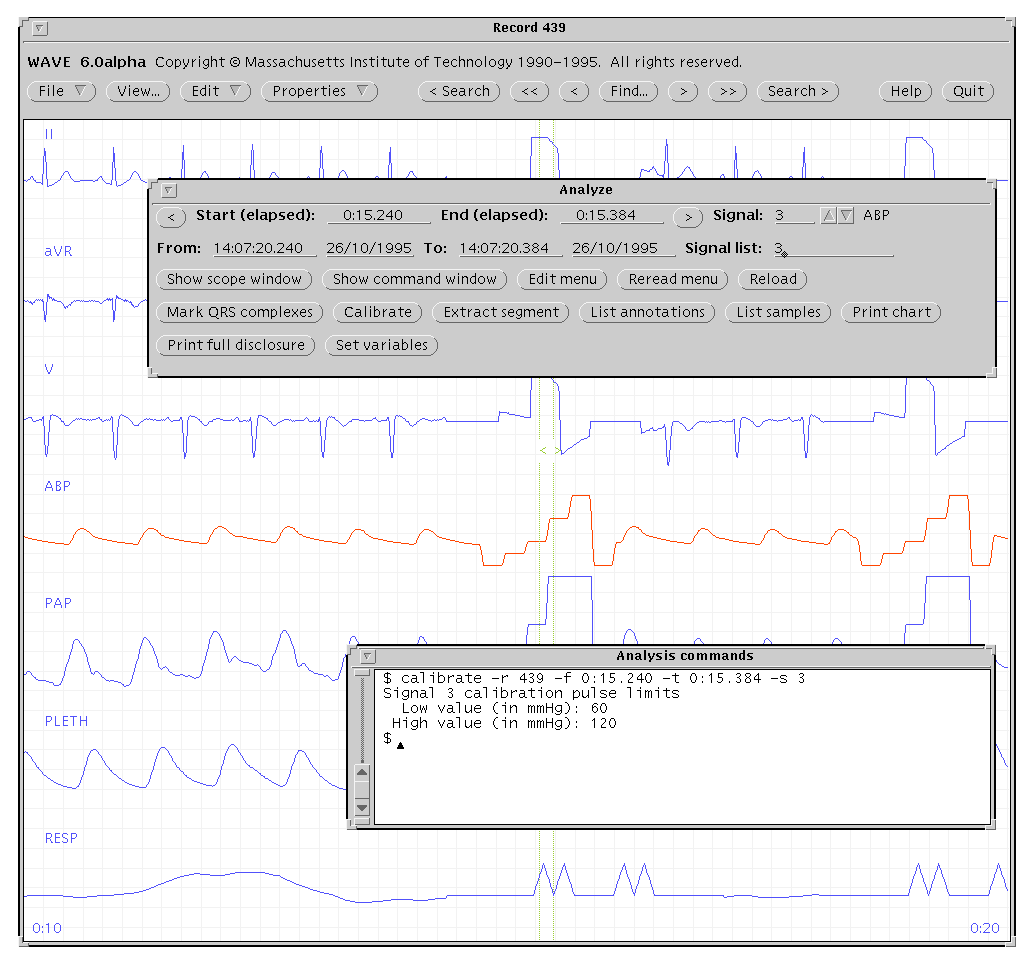
\epsfig{file=calibrate.ps}}
\caption[Signal calibration.]{Signal calibration using \WAVE{}.
Signal 3 (ABP) has been selected (note that all of the other signal
numbers have been removed from the {\sf Signal list}).  The `{\tt <}'
and `{\tt >}' markers bracket a step in the recorded calibration
pulse near the center of the signal window.  In the {\sf Analyze}
window, we have clicked on \button{Calibrate}, and the result of doing
so appears in the {\sf Analysis Commands} window.}
\label{fig:calibration}
\index{calibration}
\begin{htmlonly}
\index{analysis commands window@{\sf Analysis Commands} window}
\end{htmlonly}
\begin{latexonly}
\index{analysis commands window@{\sf Analysis Commands} window|textit}
\end{latexonly}
\end{figure}

\item
Set the {\sf Signal list} field in the {\sf Analyze} window to match
the signal(s) you have marked.  You can calibrate more than one signal
at a time if suitable calibration pulses for each signal are present
between the `{\tt <}' and `{\tt >}' markers.  Be sure to remove any
other signals from the {\sf Signal list}.

\item
Click left on \button{Calibrate} in the {\sf Analyze} window, and
answer any questions that appear in the {\sf Analysis Commands}
window.  These questions will always appear if the header file for the
record does not contain signal descriptions or physical unit
specifications; some or all of the questions may not appear if the
signal type and calibration pulse type are already known.

\item
Repeat the previous steps for any other signals that require calibration.

\item
Close and reopen the record.  (\WAVE{} does not adjust the display scales
until this has been done.)

\end{itemize}

\index{signal!calibration}\index{calibration!signal}
Figure~\ref{fig:calibration} illustrates signal calibration using a
record from the MIMIC Database.  In this case, the type of signal
(ABP) is known from an entry in the {\tt WFDBCAL} file (not shown here),
so that {\tt calibrate} is able to determine the physical units of the
signal (mmHg).  Since a variety of calibration pulses are used for ABP
signals, the {\tt WFDBCAL} file does not specify the pulse levels, which
{\tt calibrate} has asked us to enter (in this case, we have entered
{\tt 60} and {\tt 120}).  Based on this information, {\tt calibrate}
determines the offset and gain needed to convert raw sample values for
signal 3 into ABP measurements in mmHg.  {\tt calibrate} then makes
the appropriate changes to the header file for the current record.
When \WAVE{} or another WFDB application next opens this record, the ABP
signal will be properly calibrated.

\index{calibrate command@{\tt calibrate} command}
By default, {\tt calibrate} generates an amplitude histogram of the
samples between the `{\tt <}' and `{\tt >}' markers.  It then
identifies the low and high amplitude portions of the calibration
pulse by searching for the two largest distinct modes in this
amplitude histogram.  For this reason, {\tt calibrate} works best if
the segment bounded by the `{\tt <}' and `{\tt >}' markers includes at
least a few samples of both the high and low amplitude phases.  Avoid
placing either marker immediately next to the transition point between
the phases if possible.  If {\tt calibrate} fails to find two distinct
peaks in the amplitude histogram, it will produce an error message;
if this happens, adjust the positions of the markers and try again.

In some cases (for example, if the calibration pulse is a sawtooth, as
in the RESP signal at the bottom of figure~\ref{fig:calibration}),
this strategy may fail, no matter where the markers are placed.  In
such cases, try again with {\tt calibrate}'s {\tt -q} or {\tt -Q}
options to use one of its alternate algorithms.  (These are less
robust since they depend on differential rather than integrative
measurements, but they can be used in a pinch.)

For further information on signal calibration, see 
\htmladdnormallink{{\tt calibrate(1)}}{../dbag/calibr-1.htm},
in the
\htmladdnormallink{{\it WFDB Applications Guide}}{../dbag/dbag.htm}.

\section{Display calibration}

\index{display calibration}\index{calibration!display}
Display calibration is performed by \WAVE{} in several steps:

\begin{itemize}

\index{resolution!of display}
\index{dpi option for WAVE@{\tt -dpi} option for \WAVE{}}
\index{command-line options!{\tt -dpi}}\index{options!{\tt -dpi}}
\item
First, \WAVE{} determines the display resolution (either 
from the {\tt -dpi} com\-mand-line option if possible, otherwise from the
{\tt Wave.Dpi} resource if possible, or by querying the X server if
neither the command-line option nor the resource was specified).

\index{scales!time}\index{scales!amplitude}\index{time scale}
\index{amplitude scale}\index{View window@{\sf View} window}
\item
Next, \WAVE{} determines what scales to use for time and amplitude.  You
can set these using the \amenubutton{Time scale:} and \amenubutton{Amplitude
scale:} menu buttons in the {\sf View} window.  The amplitude scale refers to
standard ECG signals; the default scales (10 mm/mV and 25 mm/sec) are those
used for standard ECG chart recordings.  If you choose a non-standard amplitude
scale, \WAVE{} sets its magnification factor to the ratio between that
scale and 10 mm/mV.

\item
Finally, if any of the signals to be displayed are not ECGs, \WAVE{} checks
the WFDB calibration file (named by the {\tt WFDBCAL} environment variable) for
entries that specify the standard display scales for those signals.  \WAVE{}
multiplies these scales by its magnification factor (see above) in order to
determine the final display scales.

\end{itemize}

\index{signal!type}\index{calibration file}
\index{WFDBCAL environment variable}\index{environment variables!WFDBCAL}
\index{Load window@{\sf Load} window}
In general, it is not necessary to do anything to make \WAVE{} display
common signals at reasonable scales.  If you have a previously undefined signal
type, or you need to change the size of a particular type of signal relative to
that of an ECG, however, simply edit a copy of the WFDB calibration file, reset
{\tt WFDBCAL}, and restart \WAVE{}.  (If you wish, you need not exit and
restart \WAVE{};
\marginpar{\emph{\WAVE{} 5.0 must be restarted in this case.}}
instead, give the copy a different name, then change the
{\sf Calibration file} item in the {\sf Load} window to match.  Any changes are
effective only when the signal window is redrawn.)  See 
\htmladdnormallink{{\tt wfdbcal(5)}}{../dbag/wfdbca-5.htm},
in the 
\htmladdnormallink{{\it WFDB Applications Guide}}{../dbag/dbag.htm},
for details.

If the display calibration appears incorrect for all signals, the X
server may be supplying incorrect information about the display size
to \WAVE{}.  This problem can be diagnosed by setting the time and amplitude
scales to their default values (nominally 25 mm/sec and 10 mm/mV),
and displaying the default grid (0.5 mV x 0.2 s).  If the grid
intervals are not 5 mm in each direction, follow the procedure in
\hyperref{``How can I get correct display scales?''}
{section~}
{, page~\pageref{faq:display-scales}}
{faq:display-scales}.

\chapter{Customizing \WAVE{}}

In the previous chapters, we saw how \WAVE{}'s {\sf Analyze} window
can be modified by editing the \WAVE{} menu file.  This chapter
describes several other ways in which \WAVE{} can be customized.

\section{Using the {\sf View} window}

\begin{latexonly}
In section~\ref{sec:selecting-annotation}, we briefly opened the
{\sf View} window (see figure~\ref{fig:view-window},
page~\pageref{fig:view-window}) in order to turn on the marker bar
display.  Open the {\sf View} window again, and examine the other
controls in it.
\end{latexonly}
\begin{htmlonly}
Earlier, we briefly opened the {\sf View} window (see
figure~\ref{fig:view-window}) in order to turn on the marker bar
display.  Open the {\sf View} window again, and examine the other
controls in it.
\end{htmlonly}

Three important controls are located along the bottom edge of the
window.  \button{Redraw} makes \WAVE{} refresh the signal window,
and also closes the {\sf View} window
\index{olwm@{\tt olwm} (Open Look Window Manager)}
\index{olvwm@{\tt olvwm} (Open Look Virtual Window Manager)}
\marginpar{\emph{You will not see the pushpin unless your window
manager supports ``pinnable popups'', as do {\tt olwm} and
{\tt olvwm}.}}
(unless you have ``pinned'' it
by clicking on the pushpin at the upper left corner).  You should
click on \button{Redraw} in order to see the effects of any changes
you make in the {\sf View} window.  The other two buttons in this group are
described below.

Along the top of the window, just below the title bar, is a row of
on/off controls used to turn on various optional display elements.
These controls appear depressed (darker than the background) when they
are `on'.  The first four of these ({\sf subtype}, {\sf `chan' field},
{\sf `num' field}, and {\sf `aux' field}) control the display of
secondary fields in the annotations.  If any of these controls are
`on', the corresponding fields are displayed below each annotation
mnemonic, in the order shown in the {\sf View} window.

\index{amplitude scale}
\index{time scale}
The \amenubutton{Time scale:} and \amenubutton{Amplitude scale:}
menu buttons allow you to choose any of a wide range of standard
scales for the signal (and {\sf Scope}) windows.  Click right on
the \button{$\nabla$} to open the menu.

The \amenubutton{Draw:} menu offers the choice of displaying {\sf all
signals} (the default) or {\sf listed signals only} (i.e., those named
in the {\sf Signal list} in the {\sf Analyze} window).  By choosing to
display {\sf listed signals only}, you may rearrange the signals
within in the signal window.  By listing a signal in two or more
entries in the signal list, you can arrange to have that signal drawn
in two or more locations;  this can be useful for making side-by-side
comparisons of a signal against several others.  You may also find
it useful to remove one or more signals from the signal list in order
to reduce crowding in the signal window;  this technique is nearly essential
if the record has more than about 12 signals.  (You can also change
the spacing between signals uniformly by resizing \WAVE{}'s main window.)

\index{format!of annotation display}
The \amenubutton{Show annotations:} menu offers three ways to display
annotations: {\sf centered} (the default),  {\sf attached to signals},
and {\sf as a signal}.  If you choose {\sf attached to signals}, the
{\tt chan} field of each annotation specifies the signal number to
which the annotation is attached, and the annotation is displayed
slightly above this signal.  (Any annotations that have {\tt
chan} fields that are not valid signal numbers for the current record
are displayed at the center of the signal window.)  If you choose {\sf
as a signal}, the {\tt num} field of each annotation is taken as the
amplitude of a signal at the time of the annotation, and \WAVE{} draws
this signal in the center of the signal window by connecting the
amplitude/time pairs specified by the annotations with straight line
segments.

\index{format!of time display/entry}
\index{absolute time}
\index{elapsed time}
\index{time!display mode}
The \amenubutton{Time display:} menu provides three alternatives for
display of times in the lower corners of the signal window: {\sf
elapsed} (the default), {\sf absolute}, and {\sf in sample intervals}.
Elapsed time measures the interval in hours, minutes, and seconds from
the beginning of the record.  Absolute time (i.e., time of day and
date) is not defined for all records.  If it is available, choosing
{\sf absolute} from this menu will cause \WAVE{} to show absolute times
in the signal window, using the color \WAVE{} uses for annotations;
otherwise, \WAVE{} switches to {\sf elapsed} time display.  Times may
also be displayed {\sf in sample intervals} (counting from the
beginning of the record) for any record;  these may
be recognized in the signal window by the `{\sf s}' prefix.

\index{format!of grid display}
The choice you make from the \amenubutton {Grid display:} menu
determines how \WAVE{} draws the background grid in the signal window.
The grid intervals are fixed in time and amplitude units.  At the
default scales (25 mm/sec, 10 mm/mV) the default grid ({\sf 0.2 s x
0.5 mV}) has 5 mm intervals if the display is properly calibrated.
(If this is not the case, see
\hyperref{``How can I get correct display scales?''}
{section~}
{, page~\pageref{faq:display-scales}}
{faq:display-scales}.)
If you change the time or
amplitude scales, the grid intervals change size to match, so that you
always have a visual cue about the display scale if you leave the grid
display on.  If you choose a very small time scale (i.e., one that
permits \WAVE{} to display a large amount of data in the signal window),
the grid may appear solid grey; in this case, you may wish to choose
``{\sf 1 m x 0.5 mV}'' from this menu (so that the vertical grid lines
appear at 1-minute intervals), or `{\sf 0.5 mV}'' (thereby suppressing
the vertical grid lines), or even ``{\sf no grid}''.  At relatively
large scales, where it may be useful to have a finer grid, choose
``{\sf 0.04 s x 0.1 mV}''.  To display highly time-compressed data
with fine horizontal grid lines, choose ``{\sf 1 m x 0.1 mV}''.

If you make changes in the {\sf View} window and wish to discard them
before clicking on \button{Redraw}, you may do so by clicking on
\button{Undo changes}.  This button does not restore the initial
values if you have registered earlier changes by using
\button{Redraw};  to do this, you must restart \WAVE{}.

If, on the other hand, you have made changes in the {\sf View} window
and wish to have \WAVE{} start up with these settings, click on
\button{Save as new defaults}.  Note that \WAVE{} saves the current
state of the signal window \emph{as it appears when you click on}
\button{Save as new defaults}; if you haven't made your changes
effective using \button{Redraw}, they won't be saved.

\subsection{Highly time-compressed displays}

At highly compressed time scales (defined as any scale of 125 mm per minute or
less), \WAVE{} normally suppresses the grid display, even if you have specified
a default grid display for use at other time scales.  To change this behavior,
select the desired grid display mode, click on \button{Redraw}, and then on
\button{Save as new defaults} \emph{while viewing signals at 125 mm/min or
less}.

\subsection{Low-rate records}

Low-rate records (defined as those that are sampled at rates of 10 Hz or less)
are displayed by default at a time scale of 5 mm per minute.  To change this
default, simply change to the desired scale (all of the standard scales are
available in any case) click on \button{Redraw}, and then on
\button{Save as new defaults} \emph{while a low-rate record is open}.

\section{Resizing the signal and {\sf Scope} windows}

\WAVE{}'s main window, which contains the signal window, may be resized
using the resize ``handles'' provided by your window manager.  If you
are using an Open Look window manager such as {\tt olwm} or {\tt
olvwm}, as recommended, the resize handles are at the corners of the
window.  To use them, move the pointer over a resize handle;  when the
pointer changes shape, click left and drag it to the desired location.
(\WAVE{} adjusts the window width to the nearest multiple of one
second.)  If you use \button{Save as new defaults} in the {\sf View}
window, as described above, the new window size will be the default
for future sessions.

The {\sf Scope} window may be resized in the same way, but its default
(initial) size may not be changed.

\section{\WAVE{}~environment variables}

\index{environment variables!list of}
\WAVE{} uses many environment variables;  they are listed in this section
roughly in order of importance.  Many of them need not be set at all, since
\WAVE{} uses reasonable default values in most cases.  Those that are set
must be set on the \WAVE{} host.
\index{WAVE host@\WAVE{} host}
For general information on how to set
environment variables, see the discussion of the
\hyperref{{\tt DISPLAY} variable}
{{\tt DISPLAY} variable in section~}
{, page~\pageref{sec:setting-display}}
{sec:setting-display}.

\begin{description}
\index{DISPLAY environment variable}\index{environment variables!DISPLAY}
\item[{\tt DISPLAY}]
The name of the X server and display you are using (see
\hyperref{the worksheet}
{section~}
{, page~\pageref{worksheet}}
{worksheet}).
If not set, \WAVE{} will not be able to open windows on your display
unless your display is attached to the \WAVE{} host directly (not via
network connection).

\index{WFDB environment variable}\index{environment variables!WFDB}
\item[{\tt WFDB}]
The database path (see
\htmladdnormallink{{\tt setwfdb(1)}}{../dbag/setwfd-1.htm},
in the
\htmladdnormallink{{\it WFDB Applications Guide}}{../dbag/dbag.htm}.
If not set, \WAVE{} can find database files only in the current
directory (on the \WAVE{} host).

\index{WFDBCAL environment variable}\index{environment variables!WFDBCAL}
\item[{\tt WFDBCAL}]
The WFDB calibration file (see 
\htmladdnormallink{{\tt setwfdb(1)}}{../dbag/setwfd-1.htm} and
\htmladdnormallink{{\tt wfdbcal(5)}}{../dbag/wfdbca-5.htm},
in the 
\htmladdnormallink{{\it WFDB Applications Guide}}{../dbag/dbag.htm},
and 
\hyperref{Calibration}
{chapter~}
{, page~\pageref{ch:calibration}}
{ch:calibration}).
If not set, \WAVE{} may not scale signals other than ECGs correctly.

\index{WAVEMENU environment variable}\index{environment variables!WAVEMENU}
\item[{\tt WAVEMENU}]
The name of \WAVE{}'s
\hyperref{menu file}
{menu file (see section~}
{, page~\pageref{sec:menu-file}}
{sec:menu-file}).
If not set, \WAVE{} uses {\tt wavemenu}
in the current directory if possible; otherwise, it uses \WAVE{}'s
default menu ({\tt \$MENUDIR/wavemenu.def}).

\index{PATH environment variable}\index{environment variables!PATH}
\index{SHELL environment variable}\index{environment variables!SHELL}
\index{analysis commands window@{\sf Analysis Commands} window}
\item[{\tt SHELL}]
The command interpreter used within the {\sf Analysis Commands} window.  If
not set, \WAVE{} uses {\tt /bin/sh} (the Bourne shell).  Other shell-related
variables, such as {\tt PATH}, are also significant when \WAVE{} is running
commands within the {\sf Analysis Commands} window.

\index{EDITOR environment variable}\index{environment variables!EDITOR}
\item[{\tt EDITOR}]
The name of the text editor to be used for modifying \WAVE{}'s menu
file.  If not set, \WAVE{} uses {\tt textedit}.

\index{PRINTER environment variable}\index{environment variables!PRINTER}
\index{PostScript}
\item[{\tt PRINTER}]
The name of a PostScript printer accessible to the \WAVE{} host, to be
used for paper output.  If not set, \WAVE{} uses the default printer.

\index{PSPRINT environment variable}\index{environment variables!PSPRINT}
\item[{\tt PSPRINT}]
\index{lpr command@{\tt lpr} command}
The command needed to print PostScript from the standard input.  If
not set, \WAVE{} uses the command {\tt lpr} (or {\tt lpr -P\$PRINTER},
if {\tt PRINTER} is set).

\index{TEXTPRINT environment variable}\index{environment variables!TEXTPRINT}
\item[{\tt TEXTPRINT}]
The command needed to print ordinary text from the standard input.  If
not set, \WAVE{} uses the command {\tt lpr} (or {\tt lpr -P\$PRINTER},
if {\tt PRINTER} is set).

\index{ANNTAB environment variable}\index{environment variables!ANNTAB}
\index{annotation!table of definitions}
\item[{\tt ANNTAB}]
The name of a file that contains custom annotation definitions (see
the discussion of
\hyperref{{\tt Wave.Anntab}}
{{\tt Wave.Anntab} in section~}
{, page~\pageref{anntab}}
{anntab}
for details).  If not set, \WAVE{} uses standard annotation definitions
only.
\end{description}

The environment variables below are not needed unless the \WAVE{} binary
distribution, or XView,
\index{XView}
has been installed in non-standard directories:

\begin{description}

\index{on-line help}
\index{HELPPATH environment variable}\index{environment variables!HELPPATH}
\item[{\tt HELPPATH}]
The path for XView spot help;  if not set, \WAVE{} initializes it to
{\tt /usr/lib/help}.  \WAVE{}'s own spot help is in
{\tt \$HELPDIR/wave}, which is appended to the end of {\tt HELPPATH}
by \WAVE{}.

\index{HELPDIR environment variable}\index{environment variables!HELPDIR}
\item[{\tt HELPDIR}]
The directory in which \WAVE{}'s help directory is located;  if not set,
\WAVE{} uses {\tt /usr/local/help}.

\index{MENUDIR environment variable}\index{environment variables!MENUDIR}
\item[{\tt MENUDIR}]
The name of the directory that contains \WAVE{}'s default menu file;
if not set, \WAVE{} uses {\tt /usr/local/lib}.

\index{RESDIR environment variable}\index{environment variables!RESDIR}
\item[{\tt RESDIR}]
The name of the directory in which system-wide default X11 resource files
are kept;  if not set, \WAVE{} uses {\tt /usr/lib/X11/app-defaults}.
See the {\tt man} page for \WAVE{} for information about other
directories that are searched for resource files.
\end{description}

\section{X11 resources for \WAVE{}}

\label{sec:resources}
\index{resources}\index{X11 resources}
You can control many aspects of \WAVE{}'s appearance and behavior by
setting its resources.  If you are not familiar with this concept, refer to an
introductory book on using the X Window System, such as Quercia and O'Reilly's
{\it X Window System User's Guide}.  Since \WAVE{} is built using the XView
toolkit,
\index{XView}
all of the resources listed in the {\tt man} page for {\tt xview}
can be used with \WAVE{} (type `{\tt man xview}' for details).
If your system doesn't have an XView {\tt man} page, refer to the copy provided
with the \WAVE{} distribution
(\htmladdnormallink{{\tt xview.7}}{../dbag/xview-7.htm}).
In addition, the \WAVE{}-specific resources listed below may also be set.

The standard way to change default values of X11 resources is to
define them in a file named {\tt .Xdefaults} (note the initial `{\tt
.}') in your home directory.  \WAVE{} does this when you use
\button{Save as new defaults} in the {\sf View} panel.

If you use \WAVE{} on workstations with different display capabilities, you can
create custom resource settings for each one by moving these resource
definitions from {\tt .Xdefaults} to {\tt .Xdefaults-{\it hostname}} (where
{\it hostname} specifies the system to which the display is attached).

\begin{description}

\index{annotation!marker bars}\index{marker bars}
\item[{\tt Wave.AllowDottedLines}]
This resource specifies if \WAVE{} is allowed to render dotted lines.  \WAVE{}
normally draws annotation marker bars as dotted lines, and may use dotted
lines for other display elements on black-and-white displays for clarity.
Some X servers do not properly render dotted lines, however;  if you
observe irregular or missing annotation marker bars, change the value of
this resource from `{\tt True}' to `{\tt False}' (by editing {\tt .Xdefaults}).

\label{anntab}
\index{ANNTAB environment variable}\index{environment variables!ANNTAB}
\index{annotation!table of definitions}
\item[{\tt Wave.Anntab}]
This resource specifies the name of a file that contains a table of
annotation definitions.  The environment variable {\tt ANNTAB} can also be used
to specify this filename;  the resource overrides the environment variable
if both are set.  The file contains one-line entries of the form
\begin{verbatim}
    15 % Funny looking beat
\end{verbatim}
in which the first field specifies the (numeric) annotation code in
the range between 1 and {\tt ACMAX} inclusive (see {\tt
/usr/include/wfdb/ecgcodes.h} for a list of predefined codes and for
the definition of {\tt ACMAX}); the second field (`{\tt \%}' in the
example) is a mnemonic (used in annotation display and entry), and the
remainder of the entry is a description of the intended use of the
annotation code (which appears next to the mnemonic in the {\sf Type}
field and menu of the {\sf Annotation Template} window).  Lines in the
annotation table that begin with `{\tt \#}' are treated as comments
and ignored.  It is not necessary to specify an annotation table when
editing an existing annotation file unless previously undefined
annotation types are to be added to it during the editing process,
although it is generally harmless to do so.

\index{resolution!of display}
\index{display resolution}\index{resolution}
\index{dpi option for WAVE@{\tt -dpi} option for \WAVE{}}
\index{command-line options!{\tt -dpi}}\index{options!{\tt -dpi}}
\item[{\tt Wave.Dpi}]
This resource specifies the display resolution in dots per inch in the form
{\it mm}{\tt x}{\it nn}, where {\it mm} is the horizontal resolution and {\it
nn} is the vertical resolution.  Normally, the resolution is known to the X
server, and it is unnecessary to specify this resource.  If your X server is
misinformed, \WAVE{}'s calibrated display scales will be incorrect; the best
solution is to specify the resolution using a server option such as the {\tt
-dpi} option supported by MIT's X11 servers, since this will solve problems
common to any other applications that require calibrated scales as well.  Not
all X11 servers support such an option, however, so this option is available
as a work-around.  The command-line option {\tt -dpi} overrides the resource
if both are specified.

\index{graphics mode}
\index{display mode}
\index{g option for WAVE@{\tt -g} option for \WAVE{}}
\index{command-line options!{\tt -g}}\index{options!{\tt -g}}
\index{m option for WAVE@{\tt -m} option for \WAVE{}}
\index{command-line options!{\tt -m}}\index{options!{\tt -m}}
\index{O option for WAVE@{\tt -O} option for \WAVE{}}
\index{command-line options!{\tt -O}}\index{options!{\tt -O}}
\index{S option for WAVE@{\tt -S} option for \WAVE{}}
\index{command-line options!{\tt -S}}\index{options!{\tt -S}}
\item[{\tt Wave.GraphicsMode}]
This resource specifies the graphics mode used by \WAVE{};  it can be
overridden using the {\tt -g}, {\tt -m}, {\tt -O}, or {\tt -S} options.  The
legal values are 1 (monochrome mode), 2 (overlay greyscale mode), 4
(shared color mode), 6 (shared grey mode), and 8 (overlay color mode).

\label{setting-colors}
\index{colors!signal window}
\item[{\tt Wave.SignalWindow.\{Grey|Color\}.}{\it element}]
These resources specify the colors to be used on greyscale or color
displays.  The {\tt Color.}{\it *} resources are used only if the display is
color-capable and neither greyscale nor monochrome mode has been
specified.  {\it element} is one of {\tt Background}, {\tt Grid}, {\tt
Cursor}, {\tt Annotation}, or {\tt Signal}.  The defaults are:

\begin{center}
\begin{tabular}{lll}
{} & {\tt Grey} & {\tt Color} \\ \hline
{\tt Background} & white & white \\
{\tt Grid} & grey75 & grey90 \\
{\tt Cursor} & grey50 &	orange red \\
{\tt Annotation} & grey25 & yellow green \\
{\tt Signal} & black & blue \\
\end{tabular}
\end{center}

\item[{\tt Wave.SignalWindow.Mono.Background}]
In monochrome mode, the background is normally white, and all other
elements are normally black.  The reverse can be obtained by setting this
resource to `{\tt black}'.  (There is at least one X server for which this
fails.)

\index{Scope window@{\sf Scope} window}
\index{colors!scope window}
\item[{\tt Wave.Scope.\{Grey|Color\}.\{Foreground|Background\}}]

These resources specify the colors to be used in the {\sf Scope}
window on greyscale or color displays.  The {\tt Foreground} color is
used for the waveform and the time display; by default, it matches the
color used for signals in the signal window (see the previous item).
Some X servers do not allow the background color of the {\sf Scope}
window to be set, because of the color map animation and stippled
erasing techniques used.

\item[{\tt Wave.Scope.Mono.Background}]
This resource can be used to invert the foreground and background of
the {\sf Scope} window when \WAVE{} is running in monochrome mode.
This does not work for all X servers.

\index{signal!window!dimensions}\index{window!size}
\item[{\tt Wave.SignalWindow.\{Height\_mm|Width\_mm\}}]
These resources specify the preferred dimensions (in millimeters) for the
signal window.  The defaults are 120 and 250 respectively.

\index{font!in signal window}\index{annotation!display font}
\item[{\tt Wave.SignalWindow.Font}]
This resource specifies the font used to display annotations and time marks in
the signal window.  The default is `{\tt fixed}'.

\index{EDITOR environment variable}\index{environment variables!EDITOR}
\item[{\tt Wave.TextEditor}]
This resource specifies the name of the text editor invoked by \WAVE{} to
permit you to edit \WAVE{}'s log and analysis menu files.  The default is
{\tt textedit} (the OpenLook visual editor).  You may override this resource
by using the environment variable {\tt EDITOR}, which is also used by many
other UNIX applications that invoke editors.

\item[{\tt Wave.View.{\it showoption}}]
These resources specify which of the {\sf Show:} options at the top of the
{\sf View} window are enabled by default.  {\it showoption} is one of {\tt
Subtype}, {\tt Chan}, {\tt Num}, {\tt Aux}, {\tt Markers}, {\tt Signal
Names}, {\tt Baselines}, or {\tt Level}.  The values of these
resources are `{\tt True}' or `{\tt False}'.

\index{amplitude scale}
\index{time scale}
\item[{\tt Wave.View.{\it menuname}}]
These resources specify the positions of the initial choices in the
corresponding {\sf View} menus, where the top item on each menu is in
position 0, the one below it is in position 1, etc.  {\it menuname} is
one of {\tt TimeScale}, {\tt AmplitudeScale}, {\tt SignalMode}, {\tt
AnnotationMode}, {\tt TimeMode}, or {\tt GridMode}.  For example, to set the
initial time scale to 50 mm/sec (the item at position 6 in the 
\amenubutton{Time Scale:} menu), set {\tt Wave.View.TimeScale} to 6.

\item[{\tt Wave.View.CoarseGridMode}]
This resource specifies the initial grid display mode to be used at highly
compressed time scales (125 mm/minute or less).  The possible values are the
same as those for {\tt Wave.View.GridMode}.  The default is 0 (no grid);
recommended alternatives are 5 (1 m x 0.5 mV) or 6 (1 m x 0.1 mV).

\item[{\tt Wave.View.CoarseTimeScale}]
This resource specifies the initial time scale to be used for low-rate
records (those sampled at 10 Hz per signal or less).  The possible values are
the same as those for {\tt Wave.View.TimeScale}.  The default is 2
(corresponding to 5 mm per minute).
\end{description}

\index{XView}
\index{xrm option for WAVE@{\tt -xrm} option for \WAVE{}}
\index{command-line options!{\tt -xrm}}\index{options!{\tt -xrm}}
\index{default option for WAVE@{\tt -default} option for \WAVE{}}
\index{command-line options!{\tt -default}}\index{options!{\tt -default}}
In addition to the usual ways of setting X resources, it is possible
to set any of those listed above, as well as any of the generic XView
resources, by using the {\tt -xrm} or {\tt -default} options on the
command line when starting \WAVE{}.  For example, you can set the background
color of the signal window using a command such as
\begin{verbatim}
   wave -r 100s -xrm Wave.SignalWindow.Color.Background:lightblue
\end{verbatim}

\appendix
\chapter{Summary of \WAVE{}~controls}

This appendix contains an entry for each of \WAVE{}'s controls.
The entries appear according to the position of the controls in
left-to-right order within each window or menu.  The {\sf Annotation
Template}, {\sf Search Template}, and  {\sf Scope} window controls are
listed separately at the end.

\index{help}\index{on-line help}
This information is also available as spot help for each control
(point to the control and press the \keycap{HELP} key, or the \keycap{F1}
key if your keyboard does not have a \keycap{HELP} key).

\section{\WAVE{}'s main window}

\begin{figure}[h]
\centerline{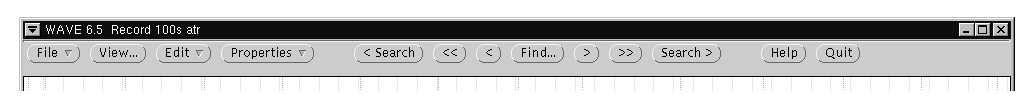
\epsfig{file=main-control-panel.ps}}
\end{figure}

\begin{description}

\index{File menu@{\sf File} menu}
\item[\menubutton{File}]
This button opens the {\sf File} menu, containing
selections for loading, saving, printing, analyzing, and logging
database files.  (See
\hyperref{File menu}
{section~}
{, page~\pageref{sec:file-menu}}
{sec:file-menu}.)

\index{View window@{\sf View} window}
\item[\button{View...}]
This button pops up the {\sf View} window, which allows you to choose
(or merely examine) display scales, grid styles, and annotation,
signal, and time display styles.  Changes are not effective until the
signal window is redrawn.  (See
\hyperref{View window}
{section~}
{, page~\pageref{sec:view-window}}
{sec:view-window}.)

\index{Edit menu@{\sf Edit} menu}
\item[\menubutton{Edit}]
The {\sf Edit} menu allows you to specify if annotation
editing is to be allowed or forbidden.  By default, editing is forbidden when
\WAVE{} starts up.  (See
\hyperref{Edit menu}
{section~}
{, page~\pageref{sec:edit-menu}}
{sec:edit-menu}.)

\index{Properties menu@{\sf Properties} menu}
\item[\menubutton{Properties}]
This button brings up the {\sf Properties} menu, with selections for obtaining
information about the current signal and annotation files and about this
version of \WAVE{}.  (See
\hyperref{Properties menu}
{section~}
{, page~\pageref{sec:prop-menu}}
{sec:prop-menu}.)

\index{Find window@{\sf Find} window}
\index{search}\index{annotation!searching for}
\item[\button{{\tt <} Search}]
This button recenters the signal window on the previous occurrence of
an annotation or marker that matches the entry in the {\sf Search for}
field of the {\sf Find} window, if any.  If no match is found, a
notice is posted, but the signal window is not recentered.  If the
{\sf Search for} field is empty, any annotation or marker will be
counted as a match.

\item[\button{\tt <<}]
This button scrolls the signal window towards the beginning of the record, by
an amount equal to the width of the signal window (i.e., a full screen).

\item[\button{\tt <}]
This button scrolls the signal window towards the beginning of the record, by
an amount equal to half of the width of the signal window.

\index{Find window@{\sf Find} window}
\index{search}\index{annotation!searching for}
\item[\button{Find...}]
This button opens the 
\hyperref{{\sf Find} window}
{{\sf Find} window (see section~}
{, page~\pageref{sec:find-window})}
{sec:find-window},
which allows you to specify what
portion of the current record should be displayed next.  You may set a specific
start or end time, or you may specify an annotation to be searched for by
\button{{\tt <} Search} and \button{Search {\tt >}} buttons.

\item[\button{\tt >}] 
This button scrolls the signal window towards the end of the record, by an
amount equal to half of the width of the signal window.

\item[\button{\tt >>}]
This button scrolls the signal window towards the end of the record, by an
amount equal to the width of the signal window (i.e., a full screen).

\index{search}\index{annotation!searching for}
\item[\button{Search {\tt >}}]
This button recenters the signal window on the next occurrence of an annotation
or marker that matches the entry in the {\sf Search for} field of the {\sf
Find} window, if any.  If no match is found, a notice is posted, but the signal
window is not recentered.  If the {\sf Search for} field is empty, any
annotation or marker will be counted as a match.

\index{on-line help}\index{Help Topics window@{\sf Help Topics} window}
\item[\button{Help}]
This button pops up the
\hyperref{{\sf Help Topics} window}
{{\sf Help Topics} window (see section~}
{, page~\pageref{sec:help-topics-window})}
{sec:help-topics-window},
containing buttons that name
several subjects for which extensive on-line help is available.  Choosing a
topic allows you to browse through or print the associated help file in a
scrollable text window.

\index{annotator name!default}
\index{Quit button@{\sf Quit} button}
\item[\button{Quit}]
\WAVE{} exits when you press this button, after saving your edits if any.
If your input file would be overwritten as a result of saving your edits, it is
first renamed by prefixing its annotator name with an underscore (`{\tt \_}').
If you have entered annotations but have not specified an annotator, the name
by which you invoked this program (normally, `{\tt wave}') is used for the
annotator name.

\end{description}

\section{The {\sf File} menu}

\index{File menu@{\sf File} menu}
\label{sec:file-menu}
Open this menu using \menubutton{File} in \WAVE{}'s main window.

\begin{description}

\index{Load window@{\sf Load} window}
\index{record!name}\index{annotator name}\index{calibration file}
\index{database path}

\item[{\sf Load}]
This selection pops up the
\hyperref{{\sf Load} window}
{{\sf Load} window (see section~}
{, page~\pageref{sec:load-window})}
{sec:load-window},
in which you can enter a new record or
annotator name, or change the name of the calibration file or the value of
the database path within this window.

\index{title bar!unsaved edit indicator}
\index{annotation file!backup}
\item[{\sf Save}]
If there are unsaved edits, this selection saves them.  The annotator name in
the title bar is marked with parentheses if there are unsaved edits.  Only one
level of backup is preserved, so you will overwrite the original annotation
file if it is in the current directory and you open the same annotator more
than once.

\index{printing!signal window contents}
\index{screen dump}
\item[{\sf Print}]
This selection prints the contents of the signal window on paper.  The output
is made from the original signal files, and therefore is of better quality than
a screen dump would be.  Your edits, if any, are saved before printing, so that
the output reflects any changes you have made.

\index{printing!commands}
\item[{\sf Print setup}]
This selection pops up the
\hyperref{{\sf Print setup} window}
{{\sf Print setup} window (see section~}
{, page~\pageref{sec:print-setup-window})}
{sec:print-setup-window},
showing the commands \WAVE{} uses
to print PostScript and text data from the standard input.

\index{menu file}
\index{Analyze window@{\sf Analyze} window}
\index{WAVEMENU environment variable}\index{environment variables!WAVEMENU}
\index{action buttons}
\item[{\sf Analyze}]
This selection pops up the
\hyperref{{\sf Analyze} window}
{{\sf Analyze} window (see section~}
{, page~\pageref{sec:analyze-window})}
{sec:analyze-window}
containing a customizable set of action buttons, and the {\sf Analysis
Commands} window (a {\tt cmdtool}-style terminal emulator).  The names
of the action buttons and their assigned actions are read
from \WAVE{}'s menu file (by default, this is {\tt wavemenu}, if it exists in the current
directory, otherwise {\tt /usr/local/lib/wavemenu.def}; the default may be
overridden by setting the environment variable {\tt WAVEMENU}
\index{environment variables!WAVEMENU}
\index{WAVEMENU environment variable}
to the name of a different file).  The buttons are usually
configured to perform various analysis functions on the current
record; read the default menu file for details.

\index{log file}
\index{pschart command@{\tt pschart} command}
\item[{\sf Log}]
This selection pops up the
\hyperref{{\sf Log} window}
{{\sf Log} window (see section~}
{, page~\pageref{sec:log-window})}
{sec:log-window},
which allows you to name a log file,
and to record in that file the current record name, the time of the
samples at the center of the signal window, and (optionally) a
one-line comment.  Log files may be used as scripts for
\htmladdnormallink{{\tt pschart}}{../dbag/pschar-1.htm}.
You may write to as many log files in a single session as you choose,
and you may accumulate entries from multiple sessions in a single log
file.
\end{description}

\section{The {\sf Load} window}
\index{Load window@{\sf Load} window}

\begin{figure}[h]
\centerline{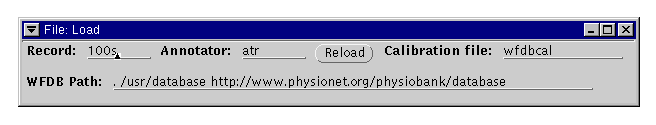
\epsfig{file=load-window.ps}}
\end{figure}
\label{sec:load-window}
Open this window by selecting {\sf Load} from the \menubutton{File} menu.

\index{record!name}
\begin{description}
\item[{\sf Record}]
Specifies the name of the record to be viewed.  The initial value of this field
is the name of the record that you specified on the command line.  To view
another record, select this field and enter another record name.

\index{annotator name}
\item[{\sf Annotator}]
Specifies the name of the annotator whose annotations are shown.  If you
specified an annotator on the command line, the annotator name is the initial
value of this field; otherwise, the field is initially empty.  Fill in or
change this field to view or edit a different set of annotations.

\index{record!reloading}
\item[\button{Reload}]
Press this button to reload the current record.  This is intended to be used
if an external process has modified the record (e.g., by writing annotations,
or by recalibrating a signal) since it was loaded into \WAVE{}.

\index{calibration file}
\item[{\sf Calibration file}]
Specifies the name of the WFDB calibration file (a text file containing
information on the relative scales of many types of signals).
Initially, this field contains the value of the {\tt WFDBCAL}
environment variable.
\index{environment variables!WFDBCAL}\index{WFDBCAL environment variable}
You should include path information in this field only if the WFDB
calibration file is not found in the WFDB path.

\index{database path}
\index{WFDB environment variable}\index{environment variables!WFDB}
\item[{\sf WFDB path}]
Specifies the search path for \WAVE{}'s input files.
Initially, this field contains the value of the {\tt WFDB} environment
variable.
\index{environment variables!WFDB}\index{WFDB environment variable}
Components are
directory names, separated by colons (`:').  An empty component (either an
initial or final colon, or two consecutive colons) specifies the current
directory.
\end{description}

\section{The {\sf Print setup} window}
\index{Print setup window@{\sf Print setup} window}

\begin{figure}[h]
\centerline{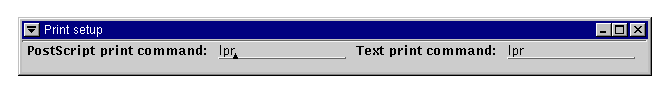
\epsfig{file=print-setup-window.ps}}
\end{figure}
\label{sec:print-setup-window}
Open this window by selecting {\sf Print setup} from the
\menubutton{File} menu.

\begin{description}
\item[{\sf PostScript print command}]
\WAVE{} supplies any PostScript data to be printed
(such as the chart generated when you choose
{\sf Print} from the \menubutton{File} menu) to the standard input
of this command.

\item[{\sf Text print command}]
\WAVE{} supplies any text to be printed (such as
on-line help) to the standard input of this
command.
\end{description}

\index{PRINTER environment variable}\index{environment variables!PRINTER}
\index{PSPRINT environment variable}\index{environment variables!PSPRINT}
\index{TEXTPRINT environment variable}\index{environment variables!TEXTPRINT}
The initial settings in the {\sf Print setup} window are determined by
the environment variables {\tt PSPRINT} and {\tt TEXTPRINT};  if
either of these variables is not set, the corresponding command is
determined by the {\tt PRINTER} environment variable (see
\hyperref{Setting up a printer for \WAVE{}}
{section~}
{, page~\pageref{sec:printer-setup}}
{sec:printer-setup}).
You may change these commands (for example, to specify
use of a different printer).  When executing commands from its menu
file, \WAVE{} replaces the strings {\tt \$PSPRINT} and {\tt
\$TEXTPRINT} with the corresponding commands from the {\sf Print
setup} window (see
\hyperref{Menu Variables}
{appendix~}
{, page~\pageref{ch:menu-variables}}
{ch:menu-variables}).

\section{The {\sf Analyze} window}
\index{Analyze window@{\sf Analyze} window}

\begin{figure}[h]
\centerline{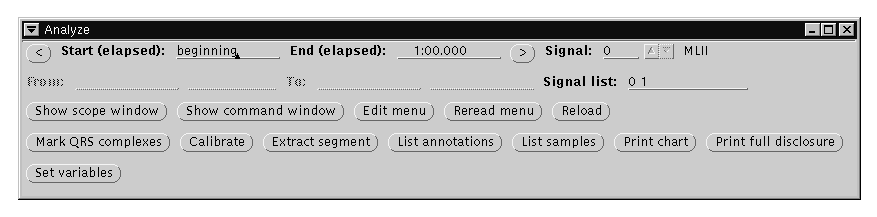
\epsfig{file=analyze-window.ps}}
\end{figure}
\label{sec:analyze-window}
Open this window by selecting {\sf Analyze} from the \menubutton{File} menu.

\begin{description}
\item[\button{\tt <}]
This button shifts the segment to be analyzed toward the beginning of the
record, by an amount equal to the length of the segment if possible.

\index{region of interest}
\index{marker!{\tt <}}
\index{elapsed time}\index{time!elapsed}
\item[{\sf Start (elapsed)}]
This field specifies (as elapsed time from the beginning of the
record) the beginning of the segment to be analyzed.  You may
enter a time directly in this field, or you may insert a `{\tt <}' marker using
the standard procedure for inserting annotations.

\index{marker!{\tt >}}
\item[{\sf End (elapsed)}]
This field specifies the end of the segment to be analyzed.  You may enter a
time directly in this field, or you may insert a `{\tt >}' marker using the
standard procedure for inserting annotations.

\item[\button{\tt >}]
This button shifts the segment to be analyzed toward the end of the
record, by an amount equal to the length of the segment.

\index{signal!number}
\item[{\sf Signal}]
This field specifies the selected signal.  You may enter a signal number
directly in this field, or you may point to a signal, depress the
\keycap{Shift} key, and click left to select the signal.  In the \WAVE{}
menu file, the symbol `{\tt \$SIGNAL}' refers to the signal number of the
selected signal; this symbol usually specifies a signal to be analyzed.  The
name of the selected signal appears to the right of its signal number.  The
uppermost signal displayed by \WAVE{} is signal 0.

\index{absolute time}\index{time!absolute}
\item[{\sf From}]
This field specifies the absolute time (and date, if defined) of the
beginning of the segment to be analyzed.  The value in this field is
updated automatically whenever the value in the {\sf Start (elapsed)}
field changes, and vice versa.  The {\sf From} field is disabled if
the current record's header does not define the absolute time of the
beginning of the record.

\item[{\sf To}]
This field specifies the absolute time (and date, if defined) of the
end of the segment to be analyzed.  The value in this field is updated
automatically whenever the value in the {\sf End (elapsed)} field
changes, and vice versa.  The {\sf To} field is disabled if the
current record's header does not define the absolute time of the
beginning of the record.

\index{signal!list}
\item[{\sf Signal list}]
This field specifies the signal list (a list of signal numbers, separated by
spaces).  In the \WAVE{} menu file, the symbol `{\tt \$SIGNALS}' refers to
the signal list; this symbol usually appears where a list of signals to be
analyzed is required.  To change the signal list, either type into this field,
or point to a signal, press and hold the \keycap{Control} key (to add the
signal to the list) or the \keycap{$\Diamond$} (or \keycap{Alt}) key (to
delete the first occurrence of the signal from the list), and click left.

\index{Scope window@{\sf Scope} window}
\item[\button{Show scope window}]
This button pops up \WAVE{}'s
\hyperref{{\sf Scope} window}
{{\sf Scope} window (see section~}
{, page~\pageref{sec:scope-window}}
{sec:scope-window},
which can be used to display a signal in `oscilloscope' mode.

\index{analysis commands window@{\sf Analysis Commands} window}
\item[\button{Show command window}]
This button pops up the {\sf Analysis Commands} window, a terminal
emulator that receives commands generated
by selecting most of the other buttons in this window, and that displays any
text output of those commands.  You may type commands directly into the window.

\index{EDITOR environment variable}\index{environment variables!EDITOR}
\index{textedit command@{\tt textedit} command}\index{menu file}
\item[\button{Edit menu}]
This button allows you to edit the \WAVE{} menu file, which
configures the analysis buttons in the {\sf Analyze} window, using the
text editor named in the {\tt EDITOR} environment variable
(or {\tt textedit} if {\tt EDITOR} is not set).  After you have saved your
changes, select \button{Reread menu} to reconfigure this window.

\item[\button{Reread menu}]
Select this button to reconfigure the {\sf Analyze} window after you
have made changes to the menu file (most easily done by
using \button{Edit menu}) or after changing records.

\item[\button{Reload}]
This button causes \WAVE{} to reload the current annotation file.  If a process
is in progress in the {\sf Analysis Commands} window, \WAVE{} defers reloading
until the process is finished.
\end{description}

\index{menu file}
\index{action buttons}
The remaining buttons in the {\sf Analyze} window perform actions
determined by the \WAVE{} menu file. If the environment variable {\tt
WAVEMENU} is set, it names that file; otherwise, the \WAVE{} menu file
is {\tt wavemenu} (if it exists in the current directory) or {\tt
/usr/local/lib/wavemenu.def}.

\section{The {\sf Log} window}
\index{Log window@{\sf Log} window}

\begin{figure}[h]
\centerline{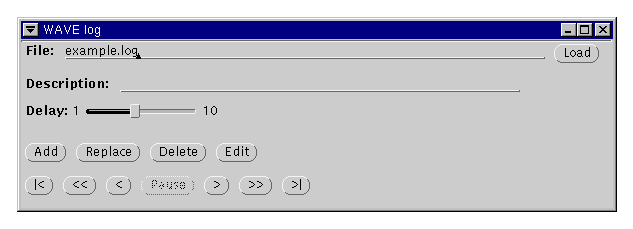
\epsfig{file=log-window.ps}}
\end{figure}
\label{sec:log-window}
Open this window by selecting {\sf Log} from the \menubutton{File} menu.

\index{log file}
\begin{description}
\item[{\sf File}]
This field names the current log file.

\item[\button{Load}]
Press this button to load (or reload) the log file if an external process
(such as one started from the {\sf Analyze} window, or an editor started using
the \button{Edit} button in the {\sf Log} window) creates or modifies the
log file.

\item[{\sf Description}]
This field contains the description associated with the current log entry.

\item[{\sf Delay}]
This slider controls the interval between display updates when a log
review is in progress.

\index{marker!{\tt :}}
\item[\button{Add}]
This button adds the current record name, the time corresponding to the
center of the signal window, and the contents of the description field, as an
entry in the log file; it also inserts an index mark (`{\tt :}') in the center
of the signal window.

\item[\button{Replace}]
This button replaces the description attached to the current log entry with the
current contents of the description field.  It does not create a new entry (use
the \button{Add} button for that purpose).

\item[\button{Delete}]
This button deletes the current entry from the log.  This button also causes
\WAVE{} to display the next log entry if it exists.

\index{EDITOR environment variable}\index{environment variables!EDITOR}
\item[\button{Edit}]
This button opens the current log file using the text editor named in the
\index{environment variables!EDITOR}\index{EDITOR environment variable}
\index{textedit command@{\tt textedit} command}
{\tt EDITOR} environment variable (or {\tt textedit} if {\tt EDITOR} is not
set).  Save your edits, exit from the editor, and click on the \button{Load}
button in the {\sf Log} window before attempting to make changes to the log
using \button{Add}, \button{Replace}, or \button{Delete}.

\item[\button{\tt |<}]
This button causes \WAVE{} to ``rewind'' the log (i.e., to show the first
log entry).

\item[\button{\tt <<}]
This button causes \WAVE{} to begin reviewing each entry in the log file in
reverse order, pausing 5 seconds between entries.  While a review is in
progress, only the \button{Pause} button is enabled.

\item[\button{\tt <}]
This button causes \WAVE{} to show the previous log entry.

\item[\button{Pause}]
This button causes \WAVE{} to stop the review of the log file that was begun
by \button{\tt <<} or \button{\tt >>}.  The \button{Pause} button is disabled
unless a review is in progress.

\item[\button{\tt >}]
This button causes \WAVE{} to show the next log entry.

\index{log file!review}
\item[\button{\tt >>}]
This button causes \WAVE{} to begin reviewing each entry in the log file,
pausing 5 seconds between entries.  While a review is in progress, only the
\button{Pause} button is enabled.

\item[\button{\tt >|}]
This button causes \WAVE{} to ``fast forward'' the log (i.e., to show the last
log entry).
\end{description}

\section{The {\sf View} window}
\index{View window@{\sf View} window}

\begin{figure}[h]
\centerline{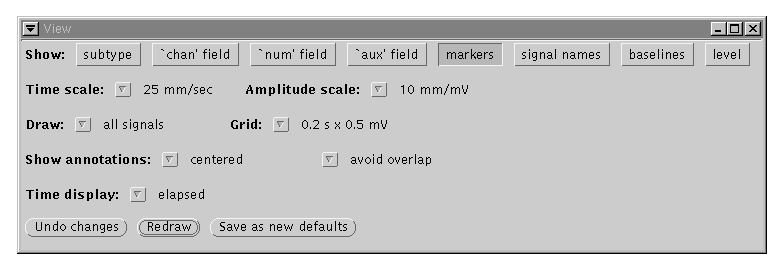
\epsfig{file=view-window.ps}}
\end{figure}
\label{sec:view-window}
Open this window using \button{View...} in \WAVE{}'s main window.

\index{annotation!mnemonic}
\index{annotation!subtyp@{\tt subtyp}}
\index{subtyp in annotation@{\tt subtyp} in annotation}
\index{annotation!chan@{\tt chan}}
\index{chan in annotation@{\tt chan} in annotation}
\index{annotation!num@{\tt num}}
\index{num in annotation@{\tt num} in annotation}
\index{annotation!aux@{\tt aux}}
\index{aux in annotation@{\tt aux} in annotation}
\index{signal!names}
\index{signal!baselines}
\index{baselines}
\index{marker bars}
\index{signal!levels}
\begin{description}
\item[{\sf Show}]
Toggle these options by selecting them.  Multiple annotation fields are shown
in the following arrangement:
\begin{quote}
{\it annotation mnemonic}\\
{\it subtype}\\
{\tt chan} {\it field}\\
{\tt num} {\it field}\\
{\tt aux} {\it field}
\end{quote}
{\sf Signal names} and {\sf baselines} are defined in the header file for the
current record.  {\sf Markers} show the precise locations of all annotations.
{\sf Levels} show the amplitudes of each signal at the time indicated by the
pointer, whenever a mouse button is depressed.  The {\sf Level} window
appears at this time.

\index{time scale}\index{scales!time}
\item[\amenubutton{Time scale:}]
Set the horizontal scale for the signal and {\sf Scope} windows by
selecting one of the choices.

\index{scales!amplitude}
\index{amplitude scale}
\item[\amenubutton{Amplitude scale:}]
Set the vertical scale for the signal and {\sf Scope} windows by
selecting one of the choices.
\end{description}

\index{grid}\index{resolution!of display}
\index{display calibration}\index{calibration!display}
\index{dpi option for WAVE@{\tt -dpi} option for \WAVE{}}
\index{command-line options!{\tt -dpi}}\index{options!{\tt -dpi}}
You can check the calibration of the display by enabling the 0.2 s x 0.5 mV
grid, and then by measuring the spacing of the grid lines.  If the spacing is
incorrect, your X server does not know the actual display resolution.  See your
X server documentation if this is the case, or use the {\tt -dpi} option when
starting \WAVE{} (start \WAVE{} with no arguments for instructions).

\begin{description}

\index{signal!display mode}
\index{signal!number}
\index{signal!list}
\item[\amenubutton{Draw:}]
Use this control to toggle \WAVE{}'s signal display mode.  By default,
\WAVE{} displays all signals in order of signal number, with signal 0 at the
top of the signal window.  If you select {\sf listed signals only}, \WAVE{}
displays only those signals that appear in the signal list (in the {\sf
Analyze} window, from top to bottom in the order in which they appear
in the signal list).

\index{format!of annotation display}
\index{annotation!display mode}
\index{chan in annotation@{\tt chan} in annotation}
\index{num in annotation@{\tt num} in annotation}
\item[\amenubutton{Show annotations:}]
Use this menu button to choose how annotations are to be displayed.  By
default, \WAVE{} displays annotations in the center of the signal window.
If you select {\sf attached to signals}, each annotation appears near the
signal specified by its {\tt chan} field.  If you select {\sf as a signal},
\WAVE{} draws a signal derived from the {\tt num} fields of any annotations
in the window, in place of the standard annotation display.

\index{format!of time display/entry}
\index{time!display mode}
\index{absolute time}
\index{elapsed time}
\item[\amenubutton{Time display:}]
By default, \WAVE{} displays elapsed time from the beginning of the record
in {\sf hh:mm:ss} format.  Use this control to select display of absolute time
(if defined for the record), or to display time in sample intervals.  If you
select absolute time display, you may enter absolute times in the {\sf Find}
window.

\index{format!of grid display}
\index{grid}
\item[\amenubutton{Grid:}]
Use this menu button to select a grid style, or to suppress the grid display.

\item[\button{Undo changes}]
This button cancels any changes you have made to the {\sf View} window
settings and restores the indicators to reflect the current settings.

\item[\button{Redraw}]
This button causes \WAVE{} to accept any changes you have made in the {\sf
View} window.  Pressing \button{Redraw} dismisses the {\sf View} window and
refreshes the signal window.

\index{Xdefaults file@{\tt .Xdefaults} file}
\item[\button{Save as new defaults}]
This button preserves the current settings within the {\sf View}
window in your home {\tt .Xdefaults} file.

\end{description}

\section{The {\sf Edit} menu}

\index{Edit menu@{\sf Edit} menu}
\label{sec:edit-menu}
Open this menu using \menubutton{Edit} in \WAVE{}'s main window.

\begin{description}
\item[{\sf Allow editing}]
This selection allows you to make changes to the annotation buffer.

\index{marker!editing}
\item[{\sf View only}]
This selection disallows annotation editing.  You may still edit `{\tt <}',
`{\sf :}', and `{\tt >}' markers.
\end{description}

\section{The {\sf Properties} menu}

\index{Properties menu@{\sf Properties} menu}
\label{sec:prop-menu}
Open this menu using \menubutton{Properties} in \WAVE{}'s main window.

\index{wfdbdesc command@{\tt wfdbdesc} command}
\begin{description}
\item[{\sf Signals...}]
This selection pops up a window containing information about the signals of the
current record, obtained by running
\htmladdnormallink{{\tt wfdbdesc}}{../dbag/wfdbde-1.htm}.

\index{sumann command@{\tt sumann} command}
\item[{\sf Annotations...}]
This selection pops up a window containing a summary of the contents of the
annotation buffer, obtained by running 
\htmladdnormallink{{\tt sumann}}{../dbag/sumann-1.htm}
(after saving any edits).

\index{WAVE version number@\WAVE{} version number}
\item[{\sf About Wave...}]
This selection pops up a window containing the version number and date of this
copy of \WAVE{}.  This window may also contain news about recent changes in
\WAVE{}.
\end{description}

\section{The {\sf Find} window}
\index{Find window@{\sf Find} window}

\begin{figure}[h]
\centerline{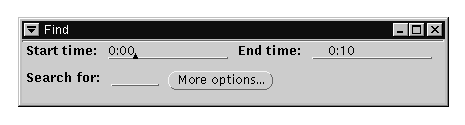
\epsfig{file=find-window.ps}}
\end{figure}
\label{sec:find-window}
Open this window using \button{Find...} in \WAVE{}'s main window.

\begin{description}

\index{View window@{\sf View} window}
\item[{\sf Start time}]
Specifies the time of the sample shown at the left edge of the signal window,
in the format specified by the {\sf Time display} item in the {\sf View}
window.  Go to any other part of the record by entering the time in this field.

\item[{\sf End time}]
Specifies the time of the sample shown at the right edge of the signal window,
in the format specified by the {\sf Time display} item in the {\sf View}
window.  Go to any other part of the record by entering the time in this field.
\end{description}

\index{format!of time display/entry}
Times can be entered in {\tt h:m:s} format, with hours or hours and minutes
omitted, or in {\tt s{\it nnnnn}} format, in which {\it nnnnn} is a number of
sample intervals from the beginning of the record.

\index{annotation!mnemonic}
\begin{description}
\index{search}\index{annotation!searching for}
\item[{\sf Search for}]
Specifies a target for  \button{{\tt <} Search} and \button{Search {\tt >}}.
Changing this field causes an immediate forward search.  The contents
of this field should match an annotation or marker mnemonic, signal quality
code, rhythm, comment, or other text string, or one of the following:

\begin{tabular*}{\textwidth}{l p{3.5 in}}
{\tt *v} & {matches any ventricular ectopic beat} \\
{\tt *s} & {matches any supraventricular ectopic beat} \\
{\tt *n} & {matches any other beat type} \\
{\tt *}  & {matches any annotation or marker} \\
{\tt .}  & {matches a deletion made during this \WAVE{} session} \\
\end{tabular*}

\index{search template window@{\sf Search Template} window}
\item[\button{More options...}]
This button clears the contents of the {\sf Search for} field and
opens the
\hyperref{{\sf Search Template} window}
{{\sf Search Template} window (see section~}
{, page~\pageref{sec:search-template-window})}
{sec:search-template-window}.
\end{description}

\section{The {\sf Help Topics} window}
\index{on-line help}\index{Help Topics window@{\sf Help Topics} window}

\begin{figure}[h]
\centerline{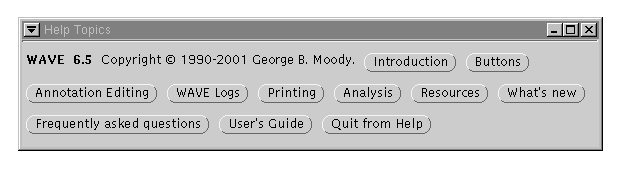
\epsfig{file=help-topics.ps}}
\end{figure}
\label{sec:help-topics-window}
Open this window using \button{Help} in \WAVE{}'s main window.

\index{help!printing}
Each of the buttons in this window, except for the last two described
below, opens a help file in a scrollable text
window.  Use the \button{Print} button in each window to get a paper
copy of the help file if you wish. The on-line manual for \WAVE{}
includes many of these files verbatim.

\begin{description}
\item[\button{Introduction}]
A quick introduction to \WAVE{}'s features.

\item[\button{Buttons}]
A summary of the functions of the buttons in \WAVE{}'s
main control panel and pop-up windows.

\item[\button{Annotation Editing}]
A summary of annotation editing procedures.

\item[\button{WAVE Logs}]
How to create and review \WAVE{} log files.

\item[\button{Printing}]
Methods for printing annotated signals from \WAVE{}.

\item[\button{Analysis}]
Using and customizing the {\sf Analyze} window.

\item[\button{Resources}]
\WAVE{}-specific X11 resources.

\item[\button{What's new}]
Recent changes in \WAVE{}.

\item[\button{Frequently asked questions}]
Common questions about \WAVE{} (answers, too!).

\item[\button{User's Guide}]
Click on this button to begin reading this guide in a web browser
window.  By default, \WAVE{} uses Netscape 1.1 or any later version
available on the \WAVE{} host.  To configure \WAVE{} to use a
different browser, see
\hyperref{\WAVE{} and the web}
{section~}
{, page~\pageref{sec:web}}
{sec:web}.

\item[\button{Quit from Help}]
Press this button to dismiss the {\sf Help Topics} window.
\end{description}

\section{The {\sf Annotation Template} window}
\index{Annotation Template window@{\sf Annotation Template} window}

\begin{figure}[h]
\centerline{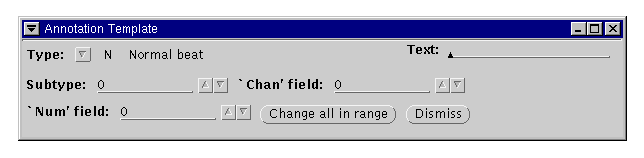
\epsfig{file=annotation-template.ps}}
\end{figure}
\label{sec:annotation-template-window}
Open this window at any time by clicking left anywhere within the
signal window.  Use the data fields in the {\sf Annotation Template}
before inserting an annotation, to specify the characteristics of the
annotation you wish to insert.

\begin{description}
\item[\amenubutton{Type:}]
This field specifies the type of annotation to be inserted.  It may be changed
by selecting a new value from the pull-down menu, by typing the mnemonic while
the pointer is within the signal window, or by selecting an existing annotation
and pressing the \keycap{Copy} or \keycap{F6} keys (these key commands also
copy the other fields of the selected annotation into the corresponding fields
of the {\sf Annotation Template}).

\item[{\sf Text}]
This field specifies the contents of the optional annotation {\tt aux} field.
It may be changed by typing into it directly or by selecting an existing
annotation and pressing the \keycap{Copy} or \keycap{F6} keys.  In most cases,
it should be empty, but it must be filled in for rhythm and certain other
non-beat annotations.  When the annotation is written, \WAVE{} prefixes the
required byte count to this field before transferring it to the {\tt aux}
field.

\item[{\sf Subtype}]
This field specifies the contents of the annotation {\tt subtyp} field.  In
most cases, it should be 0; legal values range from -128 to +127.

\item[{\sf `Chan' field}]
This field specifies the contents of the annotation {\tt chan} field.  In most
cases, it should be 0; legal values range from -128 to +127.  In multi-edit
mode, the {\tt chan} field of the annotation indicates the signal number of
the attached signal.  When inserting annotations in multi-edit mode, the value
of the {\tt chan} field in the annotation is determined by which signal is
nearest to the pointer when the insertion is performed, and the {\sf `Chan'
field} in the {\sf Annotation Template} is updated accordingly.

\item[{\sf `Num' field}]
This field specifies the contents of the annotation {\tt num} field.  In most
cases, it should be 0; legal values range from -128 to +127.  If you
have chosen to {\sf Show annotations: as a signal} in the {\sf View} window,
the {\tt num} fields of the annotations determine the signal amplitudes.

\item[\button{Change all in range}]
This button changes all annotations between the `{\tt <}' and `{\tt >}' markers
(the {\sf Start} and {\sf End} times in the {\sf Analyze} window) to match the
{\sf Annotation Template}.

\item[\button{Dismiss}]
This button makes the {\sf Annotation Template} window disappear (until it is
recalled by clicking left while the pointer is within the signal window).
\end{description}

\section{The {\sf Search Template} window}
\index{search template window@{\sf Search Template} window}

\begin{figure}[h]
\centerline{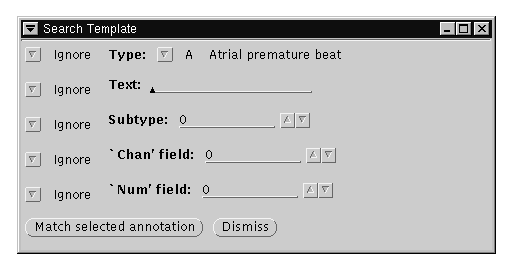
\epsfig{file=search-template.ps}}
\end{figure}
\label{sec:search-template-window}
Open this window by clicking left on \button{More Options...} in the
\marginpar{\emph{The {\sf Search Template} is not available in \WAVE{}
5.0.}}
{\sf Find} window.  This window specifies criteria for searches
performed using \button{{\tt <} Search} and \button{Search {\tt >}}.
Each of the five menu buttons at the left edge can be set to {\sf
Ignore} (the default) or {\sf Match} in order to exclude or include,
respectively, the associated annotation field in the search criteria.

The {\sf Type}, {\sf Text}, {\sf Subtype}, {\sf `Chan' field}, and
{\sf `Num' field} controls work in the same way as their counterparts
in the
\hyperref{{\sf Annotation Template} window}
{{\sf Annotation Template} window (see section~}
{, page~\pageref{sec:annotation-template-window})}
{sec:annotation-template-window}.

\begin{description}
\item[\button{Match selected annotation}]
This button copies the fields of the selected annotation (if any) into
the {\sf Search Template}, and sets all five of the menu buttons at
the left edge of the window to {\sf Match}.  This is a convenient
shortcut if you wish to find another annotation identical to a given
one.

\item[\button{Dismiss}]
This button makes the {\sf Search Template} window disappear (until it is
recalled by clicking left on \button{More Options...} in the {\sf
Find} window).
\end{description}

\section{The {\sf Level} window}
\index{Level window@{\sf Level} window}

\begin{figure}[h]
\centerline{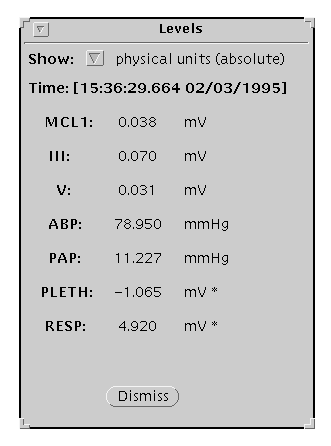
\epsfig{file=level-window.ps}}
\end{figure}
\label{sec:level-window}
Open the {\sf Level} window by choosing {\sf level} in the {\sf View}
\marginpar{\emph{The {\sf Level} window is not available in \WAVE{} 5.0}}
window, then by clicking a mouse button anywhere in the signal window.

\begin{description}
\item[\amenubutton{Show}]
Choose how time and signal levels are displayed in the {\sf Level}
window using this menu.  The four menu choices are {\sf physical units
(absolute)}, {\sf physical units (relative)}, {\sf WFDB units
(absolute)}, and {\sf WFDB units (relative)}.  Physical units are
seconds for time, and as specified in the record's header file for
each of the signals.  WFDB units are sample intervals and
analog-to-digital units (adu).  In relative mode, all measurements are
shown as differences beween the current location and the reference
location (which is determined by the placement of the `{\tt ;'}
reference marker).

\item[{\sf Time}]
This item shows the time corresponding to the most recent cursor
position while a button was depressed within the signal window (and to
the signal levels shown in the remainder of the {\sf Level} window).
Depending on the choice made using the {\sf Show} menu, this item may
be named {\sf Interval} or {\sf Sample number}.

\item[{\it Levels}]
Most of the {\sf Level} window contains an informational display
indicating the names and levels (amplitudes) of the signals.  If an
asterisk (*) appears at the end of any line, it indicates that the
corresponding signal is uncalibrated.

\item[\button{Dismiss}]
This button makes the {\sf Level} window disappear (until it is
recalled by clicking within the signal window).
\end{description}

\section{The {\sf Scope} window}
\index{Scope window@{\sf Scope} window}
\index{Analyze window@{\sf Analyze} window}
\index{oscilloscope display}
\begin{wrapfigure}{l}{2cm}
\mbox{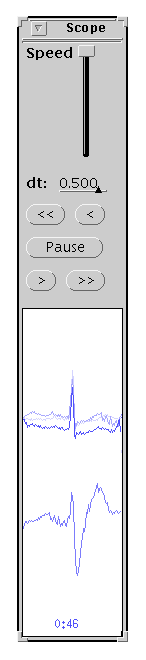
\epsfig{file=scope-window.ps,bbllx=279,bblly=390,bburx=333,bbury=530,clip=}}
\end{wrapfigure}
\label{sec:scope-window}
Open the {\sf Scope} window from the {\sf Analyze} window, using
\button{Show scope window}.  The {\sf Scope} window provides a
simulated oscilloscope display of one signal, triggered by QRS (beat)
annotations.  (Annotations that are not considered QRS annotations,
such as rhythm changes and comments, are those that appear displaced
vertically with respect to the QRS annotations in the signal window;
these non-QRS annotations do not trigger the scope display.)

\index{scales!time}\index{scales!amplitude}
\index{time scale}\index{amplitude scale}
Select the signal to be drawn in the {\sf Scope} window using the {\sf Signal}
control in the {\sf Analyze} window.  The \amenubutton{Time scale:} and
\amenubutton{Amplitude scale} controls in the {\sf View} window define the
scales used in the {\sf Scope} window.

\begin{description}
\item[{\sf Speed}]
This slider controls the playback speed.  Click left on the slider and drag it
to the desired position -- lower to reduce speed, higher to increase speed.

\item[{\sf dt}]
This field specifies the interval from the left edge of the {\sf Scope} window
to the annotated sample, in seconds.  Negative values may be used to shift the
left edge of the scope window past the annotated sample.  Drag the resize
corners to change the interval between the left and right edges of the scope
window.

\item[\button{\tt <<}]
This button displays frames continuously in reverse order.  Use \button{Pause}
to interrupt the display.  The display stops when it reaches the
beginning of the record, an index mark (`{\tt :}'), or the `{\tt <}' marker.

\item[\button{\tt <}]
This button displays the previous frame.

\item[\button{Pause}]
This button freezes the scope display.  It also forces the signal window to be
redrawn, roughly centered on the time shown at the bottom of the scope window,
with the current annotation selected.

\item[\button{\tt >}]
This button displays the next frame.

\item[\button{\tt >>}]
This button displays frames continuously in normal order.  Use \button{Pause}
to interrupt the display.  The display stops when it reaches the end of
the record, an index mark (`{\tt :}'), or the `{\tt >}' marker.
\end{description}

\chapter{System Requirements for \WAVE{}}

\label{app:system-requirements}
\index{Linux}\index{Solaris}\index{SunOS}\index{SPARCstation}\index{PC}
This section includes a shopping list of hardware and software that you will
need in order to run \WAVE{}, or that you may find useful in order to use
\WAVE{} most effectively.

\section{Necessities}

At a minimum, you will require:
\begin{description}
\item [\WAVE{} software]
This is available in binary form from MIT for SPARC-based systems
running Solaris 2.x or SunOS 4.1.x, and for PCs running Linux.  (See
\hyperref{how to obtain the current version of \WAVE{}}
{section~}
{, page~\pageref{sec:getting-wave} for details}
{sec:getting-wave}.)

\item [A computer capable of acting as a \WAVE{} host]
\index{WAVE host@\WAVE{} host}
(one for which a binary version of \WAVE{} is available).
Virtually any PC with a 386 or better CPU can run Linux, and such
systems are likely to be the least expensive choice.  Ideally, a Linux
PC to be used as a \WAVE{} host should have at least 8 Mb of RAM, at
least 200 Mb of available disk space, a three-button mouse (or
trackball), and a graphics card and monitor (17-inch or larger, with a
dot pitch of .26 mm or less) capable of non-interlaced display at 65
Hz or faster with a resolution of at least 1024x768 with 256 colors.
\index{resolution!of display}
In most cases, you will also want the system to be equipped with a
CD-ROM drive (for loading software and digitized signals) and an
Ethernet adapter or a modem.  (Check the Linux Hardware-HOWTO to be
sure that your chosen hardware is supported.  Most graphics cards,
including the popular accelerated cards, are fully supported by the standard
XFree86
\index{X Window System!XFree86 server}
X server, but a few high-end models are supported only in SVGA
compatibility mode.  Commercially available X servers for Linux
support the accelerated modes of many high-end models.)  In early
1997, it was possible to assemble a suitable Linux PC for about
US\$1000 (not including the monitor).  It is not unreasonable to budget
an equal amount for a good monitor, since \WAVE{}'s usability depends
to a significant extent on being able to see its output clearly.  If
your budget permits you to spend more, buy
extra RAM rather than a faster CPU.  Although Linux does not require
large amounts of RAM, it can use additional RAM very effectively, and
you are likely to find that purchasing (say) 16 or 32 Mb of additional
RAM results in a bigger performance improvement than spending the same
amount on a faster CPU.  Fully configured and supported Linux PCs are
available from many vendors if you prefer not to assemble your own;
see the Linux Commercial-HOWTO for further information.

SPARC-based systems available from Sun and other vendors are slightly more
expensive than comparable Linux PCs.

\item [A source of digitized signals]
\index{SPARCstation}\index{PC}\index{WFDB Software Package}\index{MS-DOS}
\index{CD-ROM}\index{ADC boards}\index{data acquisition}
Desktop SPARC systems are equipped with a single-channel
analog-to-digital converter that may be adequate for some applications
(newer versions have high-speed two-channel 16-bit ADCs).  Several
vendors supply data acquisition subsystems for SPARC systems, which
may be useful if you require more speed, resolution, or inputs.
\index{resolution!of ADC}
PC-based hardware and software for digitizing signals is available at
significantly lower cost from many vendors.  The WFDB Software Package
includes MS-DOS software for converting signals from analog to digital
form and back again, using ISA-bus ADC boards from Microstar
Laboratories (see
\hyperref{ADC boards}
{section~}
{, page~\pageref{sec:adc-boards}}
{sec:adc-boards}).
Digitized reference recordings of ECGs and
other signals are available on
\htmladdnormallink{CD-ROMs from MIT}{http://ecg.mit.edu/}
and others; several
CD-ROMs are currently available for use in basic research in
physiologic signal processing as well as for evaluation of
instrumentation.  Single CD-ROM drives are widely
available for prices ranging from US\$50 to \$300, depending on speed;
CD-ROM changers and jukeboxes are also available at higher prices.
\end{description}

\section{Printers}

\index{printing}\index{PostScript}\index{SPARCprinter}\index{Ghostscript}
All currently available \WAVE{}-compatible applications for printing
require the use of a PostScript (or compatible) printer accessible to
the \WAVE{} host
\index{WAVE host@\WAVE{} host}
system.  If you need
paper output, therefore, you should obtain a PostScript printer, or a
PostScript-compatible interpreter (such as the freely available GNU
Ghostscript) for your printer, or you should be prepared to write your
own printing applications.  For users of SBus-based SPARC systems, the
Sun SPARC\-printer is an excellent choice (less expensive and much
faster than standard PostScript printers, with better quality output).

\section{Remote access requirements}

\index{network access}\index{modem access}\index{PPP}\index{SLIP}\index{TERM}
\index{Ethernet}
In order to use \WAVE{}, you may log onto a \WAVE{} host directly, or you
may do so remotely using virtually any local system (computer or X
terminal) connected by TCP/IP-based Ethernet to a \WAVE{} host.  (PPP,
SLIP, or TERM serial-line connections also work, and may be acceptable
for viewing data, but even 28.8 Kbaud connections are likely to be
intolerably slow for extensive annotation editing.)  Thus it is
possible for several users to access \WAVE{} simultaneously using a
single \WAVE{} host, provided only that each user's computer or terminal
runs an X server.  X servers are available for virtually any computer
in current use, including those running any version of UNIX, as well
as for MS-DOS and MS-Windows PCs, Macintoshes, Amigas, and DEC VAXen
running VMS.

\index{Linux}\index{X Window System!XFree86 server}
For many users seeking to add an additional point of access to \WAVE{}, a
networked PC may be attractive.  With current CPUs and graphics adapters,
rendering speed is much faster than was available on far more expensive
workstations only a few years ago.  X server software for MS Windows 3.1/95/NT
is available from many vendors, and may be a good choice if you are heavily
invested in Windows-based software.  (For less than the cost of a Windows X
server, however, you can buy a 1 Gb disk drive and install Linux, XFree86,
and \WAVE{} on it.  Consider this before choosing a commercial X server for
Windows.)  If costs of maintenance and system administration are a concern,
an X terminal is probably a better choice than a networked PC.

\section{X11 window managers}
\index{window manager}\index{ICCCM}
Unlike other windowing systems, X does not impose a particular `look and feel'
on the user; rather, the user may select one of a number of `window managers'
that provide different user interfaces for common operations such as moving and
resizing windows.  Window managers are X client applications that have a
special status allowing them to manipulate the windows of other X clients.  Any
window manager that conforms to the ICCCM (a standard published by the X
Consortium) may be used with \WAVE{}; among these are {\tt fvwm},
\index{olwm@{\tt olwm} (Open Look Window Manager)}
\index{olvwm@{\tt olvwm} (Open Look Virtual Window Manager)}
{\tt olwm}, and {\tt olvwm},
included in source form with most Linux distributions
and widely available elsewhere ({\tt olwm} is also standard on Sun
workstations);  and {\tt mwm} (the Motif window manager, included with most
current commercial UNIX systems).  The Open Look window managers ({\tt olwm}
and {\tt olvwm}) are particularly recommended, since the others do not support
certain Open Look features of \WAVE{} (notably spot help and `pinnable'
popups).  If you
\index{X terminal}
are using an MS-DOS PC or an X terminal to access \WAVE{}, the window
manager must usually be run remotely, often on the same computer that runs
\WAVE{}.

\section{Data acquisition and digitization}
\label{sec:adc-boards}
\index{Linux}\index{digitizing signals}\index{ADC boards}
\index{sample command@{\tt sample} command (for digitization under MS-DOS)}
PC-based data acquisition is a good choice given the large number of ADC boards
available;  note, however, that Linux drivers for these boards are rare.
The WFDB Software Package available separately from MIT includes an MS-DOS
program (named {\tt sample}) for digitization and replay of analog signals
using a DAP 1200- or 2400-series data acquisition board (available from
Microstar Laboratories, 2863 152nd Avenue NE, Redmond, WA 98052 USA; telephone
+1 206 881 4286).

\index{CD-ROM}\index{MIT-BIH Arrhythmia Database}
\index{European ST-T Database}\index{MIT-BIH Polysomnographic Database}
\index{MGH/MF Waveform Database}
You may also find that an existing database of digitally recorded signals may
be useful for your studies.  Four such databases are currently available on
CD-ROM (the MIT-BIH Arrhythmia Database, the European ST-T Database, the
MIT-BIH Polysomnographic Database, and the MGH/MF Waveform Database), and
several more databases in this format are in preparation.  These disks are
compatible with any CD-ROM drive.

Note that the \WAVE{} host
\index{WAVE host@\WAVE{} host}
must be able
to read the signal files.  If you use an MS-DOS data acquisition
program, this can be accomplished in several ways:

\begin{itemize}

\item
The data acquisition PC can be set up to boot either Linux
\index{Linux}
or MS-DOS,
\index{MS-DOS}
and when running \WAVE{} under Linux, signal
files written to MS-DOS file systems can be read directly.  (Newer
versions of Linux can also read files in Windows NT, Windows 95, and
OS/2 file systems.)

\item
Alternatively, you can transfer the digitized
signals to another system acting as the \WAVE{} host, either during
digitization (by writing to a network drive) or afterwards.  Since
signal files are usually very large, Ethernet
\index{Ethernet}
transmission is
recommended.  To set up a minimal Ethernet including a Sun workstation
or Linux PC and an MS-DOS PC, you will need an Ethernet card for each
PC (usually around US\$100; Sun workstations have built-in Ethernet
adapters but may require external transceivers, usually around \$50),
TCP/IP software for the PC (such as Sun's PC-NFS, about \$300), and
miscellaneous cabling and terminators (\$20 or less).  For a truly
minimal network of only two systems, see the Linux Ethernet-HOWTO for
details on how to connect two UTP interfaces without using a hub.  You
will need a hub (US\$150 or more) to connect more than two systems,
unless you are able to use the older `thin' (10 Base 2) Ethernet.  If
\index{sample command@{\tt sample} command (for digitization under MS-DOS)}
you use {\tt sample} for digitization, signal files can be written
directly on the host system's drive at rates up to 80,000 samples per
second using PC-NFS (or up to 100,000 samples per second on local
disks).  This configuration allows you to examine the signal files
using \WAVE{} as the data are being acquired; although \WAVE{} does
not currently support real-time, continuously updated display of
incoming data, it is not difficult to create a log file for \WAVE{}
that can be used to drive a continuously updated time-delayed display
(see
\hyperref{a note about automatic scrolling}
{section~}
{, page~\pageref{sec:autoscroll} }
{sec:autoscroll}
for details).

\item
You can write digitized data to a removable disk, then read it on the
\WAVE{} host.  Devices such as IOmega's 100 Mb Zip or 1 Gb Jaz drives
are suitable for this purpose;  the SCSI versions of these devices are
usable under Linux, Solaris, and SunOS.  For high-speed or high-volume
digitization, the Jaz drive is a good choice.  An advantage of this
approach is that the removable disks are inexpensive enough to be used
for archival storage of the data.
\end{itemize}

\section{About Linux}

\label{sec:linux}
\index{Linux}
As mentioned earlier, an excellent choice for a \WAVE{}
host is a PC running Linux.  Linux is a (very) complete, and
completely free, robust, modern reimplementation of the UNIX operating
system, written by Linus Torvalds and a cast of thousands.  It is
available in source and ready-to-run form by anonymous FTP from many
sources, including
\htmladdnormallink{{\tt tsx-11.mit.edu}}{ftp://tsx-11.mit.edu/pub/linux},
\htmladdnormallink{{\tt sunsite.unc.edu}}{ftp://sunsite.unc.edu/pub/Linux}, and
\htmladdnormallink{{\tt ftp.funet.fi}}{ftp://ftp.funet.fi/pub/Linux}.
You can also obtain Linux on CD-ROMs from many
commercial sources, generally at very low prices (typically US\$10 to
\$40, depending mainly on the amount of printed documentation and
technical support offered).  Current Linux distributions include
\index{XView}\index{olwm@{\tt olwm} (Open Look Window Manager)}
\index{olvwm@{\tt olvwm} (Open Look Virtual Window Manager)}
X11R6, XView 3.2, {\tt olwm} and {\tt olvwm}, TCP/IP networking including NFS
support, the complete collection of GNU software including the GNU
C/C++ compiler, Ghostscript, \TeX, and much more.  For further
information, visit the home page of the Linux Documentation Project
(\htmladdnormallink{{\tt http://sunsite.unc.edu/mdw/}}
{http://sunsite.unc.edu/mdw/}), or get the Linux INFO-SHEET by
anonymous FTP from {\tt tsx-11.mit.edu}
(\htmladdnormallink{{\tt pub/linux/docs/INFO-SHEET}}
{ftp://tsx-11.mit.edu/pub/linux/docs/INFO-SHEET}) or from {\tt sunsite.unc.edu}
(\htmladdnormallink{{\tt pub/Linux/docs/INFO-SHEET}}
{ftp://sunsite.unc.edu/pub/Linux/docs/INFO-SHEET}).
The other Linux HOWTO documents mentioned earlier can be obtained from
these sources as well.

\index{format!of binary executable files}
Since mid-1995, Linux has supported ELF binaries, and current versions
of \WAVE{} for Linux are made available in this format.  Older
versions of Linux used the {\tt a.out} binary format.  If you have
been running one of these older versions of Linux, updating your system
to one with ELF support is highly recommended.  Until you do so, you
can use the Linux {\tt a.out} \WAVE{} version 5.4 binary available from
\htmladdnormallink{{\tt ecg.mit.edu}}{http://ecg.mit.edu/}
\begin{latexonly}
(see section~\ref{sec:getting-wave}, page~\pageref{sec:getting-wave})
\end{latexonly}.

\section{Other useful software}
\label{sec:other-software}

\index{WFDB Software Package}
\WAVE{} makes extensive use of the \emph{WFDB Software Package}, available from
the same sources as \WAVE{} itself
(\htmladdnormallink{{\tt http://ecg.mit.edu}}
{http://ecg.mit.edu}).  The WFDB Software Package includes
{\tt calibrate}, {\tt mrgann}, {\tt plot2d}, {\tt pschart}, {\tt
psfd}, {\tt rdann}, {\tt rdsamp}, {\tt sample}, {\tt snip}, {\tt
sqrs}, {\tt tach}, {\tt wfdbcollate}, {\tt wfdbdesc}, {\tt wfdbwhich},
{\tt wrann}, {\tt wrsamp}, and {\tt xform} (among many other applications).
The package also includes the WFDB library of interface functions for
user-written applications that read and write signal and annotation
files in the formats supported by \WAVE{}.

\index{Netscape}\index{web browser}
A web browser, though not a necessity for everyone who uses \WAVE{},
should be part of your software toolbox.  If you use link annotations,
you will need a browser in order to follow the links to the external
data.  Even if you don't anticipate using link annotations, you can
still use a web browser to view the on-line version of this guide.
Netscape is an attractive choice because of its simple remote-control
interface, among other reasons. As noted earlier, free copies of
Netscape for academic use or for evaluation purposes may be obtained
by anonymous FTP from
\htmladdnormallink{{\tt ftp.netscape.com}}{http://www.netscape.com}).

\index{gnuplot command@{\tt gnuplot} command}
\index{plot2d command@{\tt plot2d} command}
\index{xvgr command@{\tt xvgr} command}
An X-Y plotting program capable of being run from the command line is another
nearly essential tool.  A suitable program should be able to accept multicolumn
text input, allowing specification of which columns to plot from the
command line (so that it can be driven by \WAVE{}).  Avoid commercial software
designed for business graphics with arbitrary (often very low) limits
on the number of points that can be plotted.  If you expect to prepare
plots for publication, avoid packages that only provide screen dumps;
any decent plotting program should be able to generate plots
at the resolution of your printer.  
\htmladdnormallink{{\tt plot2d}}{../dbag/plot2d-1.htm}
(included in the WFDB Software Package) is a
bare-bones command-line front end to {\tt gnuplot}, a fairly capable
interactive plotting program that is included in most Linux distributions,
and is also available by anonymous FTP from
\htmladdnormallink{{\tt prep.ai.mit.edu}}{ftp://prep.ai.mit.edu/pub/gnu} and
numerous other sites.  An interesting alternative is {\tt xvgr},
available from
\htmladdnormallink{{\tt ftp.teleport.com/\-pub/\-users/\-pturner/\-acegr}}
{ftp://ftp.teleport.com/pub/users/pturner/acegr/} and in most Linux
distributions. \WAVE{} and {\tt xvgr} use the same Open Look/XView user
interface.

\chapter{Setting up a \WAVE{}~host}

\label{app:setup}
\section{Obtaining and installing the current version of \WAVE{}}

\label{sec:getting-wave}
\index{WAVE host@\WAVE{} host}
\index{Linux}\index{Solaris}\index{SunOS}\index{SPARCstation}\index{PC}
\index{WWW}\index{WFDB Software Package}\index{downloading}
\index{installing \WAVE{}}
Current (demo) versions of \WAVE{} for SPARCstations running SunOS and
\marginpar{\emph{
The second edition of the MIT-BIH Arrhythmia Database CD-ROM contains
\WAVE{} version 5.0 binaries for SPARC SunOS 4.1.x, within the `{\tt
src/db/wave}' directory.  The CD-ROM also contains the second edition
of this guide, which documents version 5.0, in both \LaTeX{} source
and PostScript formats.  Follow the instructions in {\tt readme.doc}
for installing the WFDB Software Package on your system.  Doing so will
install \WAVE{} 5.0 as well.
}}
Solaris, and for PCs running Linux, may be downloaded via the
Internet.  Point your Web browser to 
\htmladdnormallink{{\tt http://ecg.mit.edu}}
{http://ecg.mit.edu/}
for details, or use anonymous FTP to get
\htmladdnormallink{{\tt pub/software/README.DOC}}
{ftp://ecg.mit.edu/pub/software/README.DOC}
from {\tt ecg.mit.edu} and follow the instructions there for
downloading and installing a demo version of \WAVE{}, and the WFDB
Software Package.  (Demo versions of \WAVE{} do not permit
you to save the results of annotation editing operations, but they are
otherwise fully functional.)
\index{MIMIC Database}
Fully functional \WAVE{} binaries are also included on some of our
CD-ROMs, in the {\tt software} directory.  Follow the instructions in
{\tt software/README.DOC} to install \WAVE{} from any of these CD-ROMs.

Note that \WAVE{} cannot be run at all until the WFDB library (contained
within the WFDB Software Package) and the XView libraries ({\tt
libxview.so.3} and {\tt libolgx.so.3}) have been installed.  The
standard installation script installs the WFDB library in all cases, and
(on Linux PCs) the XView libraries if they are not already installed.
(The XView libraries are preinstalled by Sun on its current
workstations.)  It is strongly recommended that you install the
complete WFDB Software Package, since \WAVE{} uses many of the
applications included in this package.

To confirm that all necessary libraries are available on your system, type
\begin{verbatim}
    ldd /usr/local/bin/wave
\end{verbatim}
after installing \WAVE{} and the WFDB Software Package.  If no libraries
are reported as missing, the installation is complete.  Test it by
working through the exercise in chapter 1.

If you would like to try porting \WAVE{} to another operating
system for which X11 client support (Xlib) is available, please obtain
the XView
\index{XView}
source distribution and attempt to port `{\tt cmdtool}' (a
simple terminal emulator included in the XView distribution) first.
If you are successful, write to the author
(\htmladdnormallink{{\tt george@mit.edu}}{mailto:george@mit.edu})
for information on obtaining a current set of \WAVE{} sources.  Compared to
the original sources, the Linux
\index{Linux}
version of XView (freely available by anonymous FTP from
\htmladdnormallink{{\tt ecg.mit.edu}}
{ftp://ecg.mit.edu/pub/software/},
\htmladdnormallink{{\tt sunsite.unc.edu}}
{ftp://sunsite.unc.edu/pub/Linux/libs/X/xview},
\htmladdnormallink{{\tt tsx-11.mit.edu}}
{ftp://tsx-11.mit.edu/pub/linux/distributions/slackware/source/xv},
and their mirrors, and also available on many low-cost
Linux CD-ROM archives) is easier to port to another operating system,
since many Sun-specific dependencies were removed.  Nevertheless,
porting XView is likely to require significant effort.

\section{Setting up a printer for \WAVE{}}

\label{sec:printer-setup}
\index{lpr command@{\tt lpr} command}
\index{PostScript}
\index{Solaris}
\WAVE{}'s printing capabilities (see
\hyperref{Printing}
{chapter~}
{, page~\pageref{ch:printing}}
{ch:printing})
require that the \WAVE{} host be able to
print PostScript.  Your \WAVE{} host may already be set up to do this if
its default printer is a PostScript printer.  (Under Solaris, make
sure that the directory containing the BSD command {\tt lpr} is in
your {\tt PATH}.)

\index{Ghostscript}
\index{PostScript}
\index{printer!non-PostScript}
\index{fax output}
\index{format!of graphics files}
If the printer itself is incapable of rendering PostScript, you may
still be able to use it if it is supported by Ghostscript (a freely
available PostScript interpreter).  Ghostscript is included in
executable and portable C source form in most if not all Linux
distributions, and is also available by anonymous FTP from many
sources, including
\htmladdnormallink{{\tt prep.ai.mit.edu}}{ftp://prep.ai.mit.edu/pub/gnu}
and other archives of GNU software.  Ghostscript supports a wide
variety of ink jet, dot matrix,
and laser printers including popular models made by Canon, Epson,
Hewlett Packard, IBM, and others; it can also render PostScript into
files in a wide variety of graphics formats, including PBM, PGM, PPM,
PCX, and TIFF (including G3 fax format -- with a fax modem, you can
even print PostScript output on any fax machine).  Ghostscript works
by rasterizing Postscript input on the host system, then transmitting
the raster image to the printer in whatever format the printer
accepts.  For details on setting up Ghostscript for your printer, see
the documentation that comes with Ghostscript, or the Linux
Printing-HOWTO.

Assuming that the \WAVE{} host is somehow able to print PostScript
output (either directly to a PostScript printer, or via Ghostscript or
another interpreter), setup for \WAVE{} is straightforward:

\begin{itemize}
\index{PRINTER environment variable}\index{environment variables!PRINTER}
\item
Set the {\tt PRINTER} environment variable to the name of the printer
you wish to use, if that printer is not the default printer on the \WAVE{}
host.

\index{PSPRINT environment variable}\index{environment variables!PSPRINT}
\index{lpr command@{\tt lpr} command}
\item
Set the {\tt PSPRINT} environment variable to the command needed to
print PostScript from the standard input on the desired printer.
\WAVE{} assumes that this command is `{\tt lpr}' if neither {\tt PSPRINT}
nor {\tt PRINTER} are set;  if only {\tt PRINTER} is set, \WAVE{}
assumes that this command is `{\tt lpr -P\$PRINTER}'.

\index{TEXTPRINT environment variable}\index{environment variables!TEXTPRINT}
\index{on-line help}\index{help!printing}
\item
Set the {\tt TEXTPRINT} environment variable to the command needed to
print ordinary text from the standard input on the desired printer.
(This command is used, for example, to print the text of help topics.)
\WAVE{} assumes that this command is `{\tt lpr}' if neither {\tt TEXTPRINT}
nor {\tt PRINTER} are set;  if only {\tt PRINTER} is set, \WAVE{}
assumes that this command is `{\tt lpr -P\$PRINTER}'.

\index{printer!resolution}
\index{resolution!of printed output}
\item
Finally, if your printer is capable of resolution higher than 300 dpi,
you may also wish to add appropriate {\tt -d} options to the {\tt
pschart} and {\tt psfd} commands in \WAVE{}'s menu file (see
\hyperref{Creating custom formats for printing}
{section~}
{, page~\pageref{sec:custom-printing}, for details}
{sec:custom-printing}).
(This is not necessary in order to obtain
properly-scaled output, but this will affect the amount of fine detail
in your plots, and the thickness of the plotting lines.)
\end{itemize}

\index{profile@{\tt .profile}}
\index{login@{\tt .login}}
In most cases, you will want to add the commands needed to set these
variables to your {\tt .login} or {\tt .profile} file on the \WAVE{}
host, so that they are executed automatically whenever you log in.
For details on setting environment variables, see the discussion of the
\hyperref{{\tt DISPLAY} variable}
{{\tt DISPLAY} variable in section~}
{, page~\pageref{sec:setting-display}}
{sec:setting-display}.

\index{printing!remotely vs. locally}
If you are using \WAVE{} remotely, you may prefer to use a local printer
for your output.  \WAVE{} has no specific support for doing so, but this
can often be arranged if, for example, your own computer is able to
make its printer available for printing from the \WAVE{} host (this is
can be done easily if your computer runs any version of UNIX, or with
somewhat more difficulty if it runs Microsoft Windows).  In this case,
usually all that is needed is to set {\tt PRINTER} to the name of your
printer (as it is known to the \WAVE{} host).  Another possibility is to
set {\tt PSPRINT} and {\tt TEXTPRINT} to commands that capture output
in a file, and then transfer the file to your own computer (via FTP or
any other method) for local printing.  For example, you might set {\tt
PSPRINT} to `{\tt cat~>>output.ps}' and {\tt TEXTPRINT} to `{\tt
cat~>>output.txt}'.  These commands accumulate all PostScript output
into {\tt output.ps}, and all text output into {\tt output.txt}, so
you should delete these files from the \WAVE{} host after copying them
to your computer, so they don't grow indefinitely.

If you need to change printers or print commands while running
\WAVE{}, this can be easily accomplished within \WAVE{}'s
\hyperref{{\sf Print setup} window}
{{\sf Print setup} window (see section~}
{, page~\pageref{sec:print-setup-window})}
{sec:print-setup-window},
which may be opened by selecting {\sf Print setup} from the
\menubutton{File} menu.

\chapter{Frequently Asked Questions}

This is the \WAVE{} FAQ (frequently asked questions) list.  If your version of
\WAVE{} is newer than this guide, you may wish to review the on-line copy of
this FAQ (click on \button{Frequently Asked Questions} in \WAVE{}'s
{\sf Help} window).

If your question is not on this list, and you think it should be, please
send it to me
(\htmladdnormallink{{\tt george@mit.edu}}
{mailto:george@mit.edu})!

\section{Hardware questions}

\subsection{Can I use \WAVE{} if I don't have a SPARCstation?}

If you have a 386, 486, or Pentium-based PC with a VGA card, mouse, at
least 8 Mb of RAM and 100 Mb of available disk space, you can run
\WAVE{} under Linux,
\index{Linux}
a freely available UNIX clone for the PC.

If you have any networked computer that can run X11R4 or a later version
(this includes all current UNIX workstations, PCs, Macintoshes, and a variety
of other systems), and access via network to either a SPARCstation or a
PC running Linux, you can run \WAVE{} remotely (see the next question).

Otherwise, you're out of luck at present.  \WAVE{} requires X11R4 or
later and the XView
\index{XView}
toolkit (both are freely available
in source form for UNIX systems).  See
\hyperref{Setup}
{Appendix~}
{, page~\pageref{app:setup},}
{app:setup} for details if you would like to try porting
\WAVE{} to another version of UNIX.

\index{PostScript}
Other WFDB applications ({\sf WVIEW} for Microsoft Windows, {\sf VIEW} for
MS-DOS, {\sf MacView} for the Macintosh, and {\tt pschart}
and {\tt psfd} for PostScript devices) offer many of the display features of
\WAVE{} in other environments;  none of these currently support annotation
editing or control of external programs, however.

\subsection{How can I use \WAVE{} from an X terminal, PC, Mac, etc.?}

\index{remote access}\index{network access}
As with any X application, you can use an X terminal or any system equipped
with an X server to interact with a copy of \WAVE{} running on another computer
connected to the same network.  To do so, however, requires a few additional
steps:

\begin{itemize}
\item
Find out the host names of the two systems.  On a UNIX system, the
`{\tt hostname}' command will give you this information.  If your
display is connected to a PC or other non-UNIX system, you can try
remotely logging onto the UNIX system on which \WAVE{} resides, and
using the `{\tt who}' command to discover the name of the system in
front of you.

\item
Assume that your system is named {\tt hither} and that \WAVE{} resides on 
{\tt yon}.
\index{WAVE host@\WAVE{} host}
\index{IP address}
\index{address, IP (Internet Protocol)}
You may need to add {\tt yon} to the X server access control list
on {\tt hither}, in order to make it possible for X clients on {\tt yon} to
open windows on your screen.  If {\tt hither} is a UNIX system, you can
accomplish this by typing (on {\tt hither}) `{\tt xhost +yon}'.  (Note:  if
{\tt hither} doesn't recognize {\tt yon} by name, this command will have no
effect.  In this case, use {\tt yon}'s IP address in place of its name.)

\item
Remotely log in to {\tt yon} (for example, via {\tt telnet}), and set the
{\tt DISPLAY} environment variable on {\tt yon} to point back to your display.
If you use the C-shell on {\tt yon}, this will normally be done by
`{\tt setenv DISPLAY hither:0.0}'.  Users of {\tt sh}, {\tt ksh}, or {\tt bash}
should type `{\tt DISPLAY=hither:0.0; export DISPLAY}'.  (Note:  if {\tt yon}
doesn't recognize {\tt hither} by name, this command won't work.  In this case,
use {\tt hither}'s IP address in place of its name.)

\item
Check the connection by starting an X11 client such as {\tt xterm} on {\tt
yon}.  A new window should appear on your display within a few seconds.  (See
the documentation for your X server if this doesn't work).

\item
Once you have succeeded in the test in the previous step, start \WAVE{}
in the usual way (`{\tt wave -r} \emph{record ...}') on {\tt yon}.
See 
\hyperref{``Where do I find the missing fonts?''}
{``Where do I find the missing fonts?'' (section~}
{, page~\pageref{faq:missing-fonts})}
{faq:missing-fonts}
if your X server complains about missing fonts.  See
\hyperref{``I can't find the file named \emph{record}!''}
{``I can't find the file named \emph{record}!'' (section~}
{, page~\pageref{faq:cannot-find-record})}
{faq:cannot-find-record}
if \WAVE{} complains about missing files.
\end{itemize}

X servers are standard on all current UNIX workstations, but not on
PCs or Macintoshes.  There are many MS Windows-hosted X servers
available commercially, as well as a smaller number of MS-DOS and
Macintosh-hosted X servers.

\subsection{Can I run \WAVE{} remotely using a modem?}

\index{modem access}\index{PPP}\index{SLIP}\index{TERM}
It is possible, with appropriate (SLIP, PPP, or TERM) software, to run
\WAVE{} across a serial connection (see the previous question for
details), but this will be painfully slow even with a 28.8 kbps modem.
Using \WAVE{} remotely via Ethernet is usually quite tolerable,
however.

\subsection{How can I insert annotations using a two-button mouse?}

\index{mouse!middle button!simulating}
\index{middle mouse button!simulating}
\index{mouse!right button!simulating}
\index{right mouse button!simulating}
\index{chording (mouse technique)}
Normally, the middle button is used to insert annotations, so the problem is
to simulate a middle button click if you don't have a middle button.
Most, if not all, X servers that support two-button mice provide a way to do
this.  The most common method is to press both buttons simultaneously (an
operation sometimes called ``chording,'' by analogy with playing a chord on
the piano).  Typically, you have an adjustable window of 50 to 100 milliseconds
in which to press both buttons, so that you don't need exactly simultaneous
clicks (which would be impossible to achieve reliably).  Some X servers delay
reporting a button-down event until a button-up event occurs;  this approach
makes chording less error-prone, but it means that the feedback that \WAVE{} 
produces in response to button-down events gets delayed until it may no longer
be useful.  Another approach, more commonly used with one-button mice, is to
simulate the middle button (and, if necessary, the right button) using a
mouse button and keyboard key combination, such as clicking while pressing the
\keycap{SHIFT} or \keycap{CTRL} keys.  Check your X server's manuals for
information about which of these methods is supported.  With a little practice,
annotation editing can be tolerable with a button-impaired mouse.

Independent of the X server, \WAVE{} also makes it possible to simulate a
middle button click, by using the \keycap{F2} key (or the \keycap{5} key
on the numeric keypad).  If you use this technique, you might also wish to
use the \keycap{F3} and \keycap{F4} keys to drag the pointer and marker bars
left or right.

Inexpensive three-button mice, trackballs, and touchpads manufactured
by Logitech and many others are widely available for PCs, and are
highly recommended if you do much annotation editing.  Most are fully
compatible with Microsoft two-button mice and with X server software
for PCs.  Some users prefer trackballs for precision editing since
there is no tendency for the pointer to move when clicking the
buttons, as with a mouse.

\subsection{How do I get spot help if I don't have a {\sf Help} key?}

\index{on-line help}\index{help}
\label{faq:no-help-key}
If you are not using \WAVE{} with a Sun keyboard, use the \keycap{F1}
key to open XView
\index{XView}
spot help for \WAVE{}.  If this doesn't work, you
may need to use the `{\tt xmodmap}' utility (a standard component of
X11, usually found in the same directory as other X clients such as
`{\tt xterm}').  Try the following command:

\begin{verbatim}
	xmodmap -e "keysym F1 = Help"
\end{verbatim}

If you are now able to use \keycap{F1} to open spot help, you may wish
to include this command in your `{\tt .xinitrc}' (a text file in your
home directory; create it if it doesn't exist) so that spot help via
\keycap{F1} is enabled whenever you log in.

If you are not using {\tt olwm} or {\tt olvwm},
\index{olwm@{\tt olwm} (Open Look Window Manager)}
\index{olvwm@{\tt olvwm} (Open Look Virtual Window Manager)}
spot help may not work
properly; in particular, your window manager may pass incorrect
information about which window is active when you invoke spot help.
There is no general solution to this problem; try using {\tt olvwm} or
{\tt olwm}, at least until you are familiar with \WAVE{}'s controls.

\section{Problems starting \WAVE{}}

\subsection{Why won't \WAVE{} run?}

Here are a few things to check:

\begin{enumerate}
\item
\index{wave command@{\tt wave} command}
\index{record!name}
\index{annotator name}
The command used to run \WAVE{} must be typed in lower case, as in `{\tt
wave -r 100s -a atr}'.  Note that letters in record names and
annotator names are also usually in lower case.

\item
\index{PATH environment variable}\index{environment variables!PATH}
Try typing {\tt wave} with no command-line arguments.  You should see a summary
of options.  If you don't, {\tt wave} has not been installed properly, is not
in your {\tt PATH}, or another program named {\tt wave} is in your {\tt PATH}.

\index{dynamically linked libraries}
\index{shared libraries}
\index{libraries!missing}
\index{LD\_LIBRARY\_PATH environment variable}
\index{environment variables!LD\_LIBRARY\_PATH}
Errors similar to `{\tt wave: can't load library 'libxview.so.3'}'
indicate an installation problem which is probably shared by other
applications that use the same libraries.
Use the command `{\tt ldd `which wave`} to identify which dynamically
linked libraries are missing.  Locate these on your system (for
example, using a command such as `{\tt find / -name libxview.so.3
-print}';  if any of these libraries cannot be found on your system, it may be
downloaded from \htmladdnormallink{MIT}{http://ecg.mit.edu}.)
Add the directories in which the missing libraries are found to your
{\tt LD\_LIBRARY\_PATH}.  For example, if the missing libraries are
located in {\tt /usr/openwin/lib}, and you are using the C-shell, use the
command `{\tt setenv LD\_LIBRARY\_PATH /usr/openwin/lib:\$\{LD\_LIBRARY\_PATH\}}'.
Under Linux, if you can obtain root permissions, a more permanent
solution is to add {\tt /usr/openwin/lib} to the list of directories
in `{\tt /etc/ld.so.conf}', and then to run {\tt ldconfig}.

\item
If the previous test works, try typing `{\tt wave -r 100s -a atr}'.  (All
\WAVE{} distributions come with record 100s.)  One of the following should
happen:
\begin{itemize}
\item
\index{WFDB environment variable}\index{environment variables!WFDB}
\index{DISPLAY environment variable}\index{environment variables!DISPLAY}
If you see a summary of options, rather than the \WAVE{} main window, read
the message carefully;  you may not have set the {\tt DISPLAY} or {\tt WFDB}
environment variables, or the X server may not be running.

\item
If you see a lengthy error message referring to missing fonts, see
\hyperref{``Where do I find the missing fonts?''}
{``Where do I find the missing fonts?'' (section~}
{, page~\pageref{faq:missing-fonts})}
{faq:missing-fonts}.

\item
If you see neither a summary of options nor the \WAVE{} main window, the
{\tt DISPLAY} environment variable may be set incorrectly, the X server may be
refusing permission to open a window, or your window manager may be waiting
for you to specify the location or size of the window to be opened.

\item
If you see only a message box reading `{\sf Record 100s is unavailable}', your
{\tt WFDB} environment variable may be set incorrectly;  in this case, find the
directory (probably {\tt /usr/local/database}) containing a file named
`{\tt 100s.hea}' and append the name of that directory to the value of
{\tt WFDB}.

\item
\index{signal!window}
If \WAVE{}'s signal window appears, but is solid white, your X server has a
bug. Click on any of the navigation controls (e.g., \button{\tt <<},
\button{\tt <}, \button{\tt >}, or \button{\tt >>}), or resize the window,
to make the signals appear.  If the signal window is solid (or nearly solid)
blue or black, or has only horizontal lines across it, see
\hyperref{``I can't see the signals!''}
{``I can't see the signals!'' (section~}
{, page~\pageref{faq:cannot-see-signals})}
{faq:cannot-see-signals}.

\index{S option for WAVE@{\tt -S} option for \WAVE{}}
\index{command-line options!{\tt -S}}\index{options!{\tt -S}}
\item
If the signals appear, but there are no annotations or time stamps in the
signal window, your X server has a (different) bug.  Restart \WAVE{}, adding
the `{\tt -S}' option to the `wave' command.  Also see
\hyperref{``I can't see text in the signal window!''}
{``I can't see text in the signal window!'' (section~}
{, page~\pageref{faq:cannot-see-text})}
{faq:cannot-see-text}.

\item
If you see a correct display, your problem is specific to the record you
were previously trying to view.  Find the directory containing the header
file for the desired record, and append the name of that directory to the
value of {\tt WFDB}.  If the record is on a CD-ROM, or was copied from a CD-ROM,
its header file is `\emph{record}{\tt .hea}' (where \emph{record} is the record
name);  otherwise, its name is probably `{\tt header.}\emph{record}'.
\end{itemize}
\end{enumerate}

\subsection{Where do I find the missing fonts?}

\label{faq:missing-fonts}
\index{Open Look fonts}\index{font!Open Look}
\WAVE{} is an XView
\index{XView}
application, and requires the Open Look cursor font
on the server.  If your server doesn't have this font (`{\tt
olcursor.snf}' for X11R4 and earlier servers, `{\tt olcursor.pcf}' for
X11R5 and later servers), you must install it before \WAVE{} will run.
XView applications also use the `{\tt olgl??.snf}' or `{\tt olgl??.pcf}'
glyph fonts; if these are missing, \WAVE{} will run but certain standard
Open Look graphical elements will not have the correct appearance.  To
install these fonts on your X server's system:

\begin{enumerate}

\item
Generate copies of `{\tt ol*.snf}' or `{\tt ol*.pcf}' for your X server
system's architecture.

\item
Copy `{\tt ol*.snf}' or `{\tt ol*.pcf}' to a world-readable directory on the
server machine.

\item
Update the font database on the server machine.

\item
Force the server to reread the font database.
\end{enumerate}

You should be able to find `{\tt ol*.snf}' or `{\tt ol*.pcf}' files on the
machine on which \WAVE{} resides (probably in {\tt /usr/lib/X11/fonts/misc}).
The `{\tt ol*.pcf}' files are portable (although usually optimized for the
architecture of the system on which they are installed).  If you need to use
`{\tt snf}' fonts, however, and the server machine is not of the same
architecture, it will be necessary to find `{\tt ol*.bdf}' in the XView
\index{XView}
distribution and use `{\tt bdftosnf}' to generate `{\tt .snf}' files
for your X server system's architecture (see the man page for `{\tt bdftosnf}';
this step can be done trivially on the server machine, if `{\tt bdftosnf}' is
available there, or with a little more trouble on the remote machine).  If the
server machine runs UNIX, read the man pages for `{\tt mkfontdir}' and
`{\tt xset'} to see how to update and reread the font database; otherwise,
consult the documentation for your X server.  Note that (under UNIX) you do
not need to have write permission in the standard font directory in order to
perform these steps; if you add your own font directory to the font path using
`{\tt xset}', however, remember that this setting lasts only until the server
exits and will need to be repeated afterwards.

\section{Display-related questions}

\subsection{I can't see the signals!}

\label{faq:cannot-see-signals}
\index{signal!window}
If the signal window is solid white, your X server has a bug.  Click on any of
the navigation controls (e.g., \button{\tt <<}, \button{\tt <}, \button{\tt >},
or \button{\tt >>}), or resize the window, to make the signals appear.

\index{format!of signal files}
If the signal window is solid or nearly solid blue (or black if you have
a mono\-chrome or greyscale display), the signals are too big.  \WAVE{}
may be attempting to display signals that fill the entire window.  In
rare cases, noise in the signals themselves can produce this effect.
More common causes include incorrect signal format or gain
specifications in the header file for the record you have opened,
\index{amplitude scale}\index{scales!amplitude}
incorrect display calibration, or a choice of amplitude scale that
results in excessive vertical range of one or more signals.  This
effect can also occur as a result of various problems related to the
WFDB calibration file, for example, if the {\tt WFDBCAL} environment
\index{WFDBCAL environment variable}\index{environment variables!WFDBCAL}
variable does not name an accessible WFDB calibration file (see 
\htmladdnormallink{{\tt wfdbcal(5)}}{../dbag/wfdbca-5.htm}
for details), if any of the signals in the record are of
types not listed in the WFDB calibration file, or if the WFDB calibration
file does not contain appropriate default display scales for all of
the signal types in the record.  See the next several questions for
suggestions on correcting these problems.

If the signal window contains horizontal lines (in blue if you have a color
display) where the signals should appear, the signals are too small.  In this
case, the signal gains specified in the header file may be incorrect, the
display calibration may be incorrect, or you may have specified an amplitude
scale that reduces the vertical range of the signals to zero.  Click on
\button{View...} to check the scales, and adjust them if necessary.

If the signal window contains time indicators in the lower corners,
look for the signal names along the left edge of the window.  If there
are no signal names visible, click on \button{View...}, then on {\sf
signal names} and \button{Redraw} in the {\sf View} window.  If signal
names still do not appear, either the header file or the signal file
for the record you have opened may be inaccessible.  Find these files
(see the next question), add the directory that contains them to your
WFDB path, and try to read a few samples using `{\tt rdsamp -r \emph{
record} -t 1}'.  If this fails, examine the header file for the record
(a text file), and be sure that it specifies at least one signal in an
accessible signal file.

\subsection{I can't see text in the signal window!}

\label{faq:cannot-see-text}
\index{S option for WAVE@{\tt -S} option for \WAVE{}}
\index{command-line options!{\tt -S}}\index{options!{\tt -S}}
This may result from an X server bug.  This bug appears to be limited
to X servers that support `true color' (typically 24- or 32-bit) displays,
when using overlay graphics.  Restart \WAVE{}, adding the `{\tt -S}'
option to the end of the `{\tt wave}' command.

\index{Netscape!color map problem with}\index{color map}
This problem may also occur on 8-bit `pseudo-color' displays, if another
application such as Netscape has already allocated most of the color map.
To avoid this problem, start \WAVE{} before starting Netscape.

\subsection{\WAVE{} doesn't draw/erase properly in the scope window!}

\index{Scope window@{\sf Scope} window}
\marginpar{\emph{Some X servers have bugs that interfere with both of
the scope display methods used by \WAVE{} 5.0.  If changing display
modes doesn't help, try using a current version of \WAVE{}.}}
This problem may result from several different X server bugs.  You
may be able to avoid it by switching from overlay graphics mode (the
usual default) to shared color mode (selected using \WAVE{}'s {\tt -S}
\index{S option for WAVE@{\tt -S} option for \WAVE{}}
\index{command-line options!{\tt -S}}\index{options!{\tt -S}}
command-line option), or vice versa, since \WAVE{} uses different
techniques for drawing in the scope window depending on the display
mode.

\subsection{How can I get correct display scales?}

\label{faq:display-scales}
\index{xdpyinfo command@{\tt xdpyinfo} command}
\index{resolution!of display}
Use `{\tt xdpyinfo}' (a standard X client that is provided as part of
the X core distribution) to check several server parameters.  (As with
virtually all X clients, it doesn't matter which machine you find
`{\tt xdpyinfo}' on; it will query your server from wherever it is run.)
`{\tt xdpyinfo}' will report the version and release numbers of your server;
you should have version 11, release 3 or later.  It will also report
the screen size in pixels and the resolution in pixels per inch.  Take
a minute to verify the screen resolution by direct measurement of the
screen with a ruler.  If the resolution reported by `{\tt xdpyinfo}' is
incorrect, \WAVE{} will not be able to draw waveforms at properly
calibrated scales.  The sample X11 servers from MIT all support a
\index{dpi option for WAVE@{\tt -dpi} option for \WAVE{}}
\index{command-line options!{\tt -dpi}}\index{options!{\tt -dpi}}
`{\tt -dpi}' option, which allows you to specify the correct screen
resolution at the time the server is started; read the man page for X
for details.  (If your server does not support this feature, \WAVE{} can
be given a similar `{\tt -dpi}' option.)

\index{display calibration}\index{calibration!display}
You can also double-check your display calibration using \WAVE{} itself.
Run \WAVE{}, enable the grid display, and set the display scales to
their default values (25 mm/sec, 10 mm/mV).  (Click on
\button{View...} to pop up the controls for the grid and the display
scales; remember that any adjustments you make become effective only
after you click on \button{Redraw} within the {\sf View} window.)  The
grid intervals should measure exactly 5 mm in each direction.  If they
are too small, use a larger value for the `{\tt -dpi}' specification; if the
grid lines are more than 5 mm apart, decrease the `{\tt -dpi}' values.

\subsection{Why are signals too big or too small?}

\index{signal!calibration}\index{calibration!signal}
There are several reasons why the size of signals may be incorrect.  \WAVE{}
determines display scales for signals based on several parameters:

\begin{itemize}

\item
\index{WFDBCAL environment variable}\index{environment variables!WFDBCAL}
First, the {\tt WFDBCAL} environment variable specifies the name
of a text file (located in a directory in the WFDB path) containing the
names of many common signals and customary display scales for each
(expressed as physical units per centimeter).  For example, ECG
signals are customarily displayed at a scale of 1 mV per centimeter.
If a signal appears at an inappropriately large or small scale, its
name may be missing from the calibration file, the {\tt WFDBCAL}
variable may not correctly specify the name of the calibration file,
or the {\tt WFDBCAL} file may not reside in a directory in the WFDB path.
On most systems, the calibration file is `{\tt
/usr/local/database/wfdbcal}', and the {\tt WFDBCAL} environment
variable is set by the same command used to set the WFDB path (see the
discussion about the
\hyperref{database environment}
{database environment in section~}
{, page~\pageref{sec:wfdb-path}}
{sec:wfdb-path}).
Instructions for adding additional signal names and scales to the calibration
file are located within the file itself, and may also be found in the
\htmladdnormallink{{\it WFDB Applications Guide}}{../dbag/dbag.htm}.

\item
\index{header file}
Second, the header file for the record specifies the gain for each signal
(the number of analog-to-digital units per physical unit).  If the gain has
not been determined, or is incorrect, the size of the signal as drawn by
\WAVE{} may be incorrect as well.  If you know the physical values that
correspond to at least two levels represented in the signal (for example,
the top and bottom of a calibration pulse), you can use the `{\tt calibrate}'
application to determine the gain and to rewrite the header file.  See the
\htmladdnormallink{{\it WFDB Applications Guide}}{../dbag/dbag.htm}
for details.  `{\tt calibrate}' can be most conveniently run from
\WAVE{}'s {\sf Analysis} window.

\item
Finally, the display calibration determines the number of pixels per inch
(25.4 mm).  \WAVE{} usually gets its information about the display calibration
from the X server, but the X server may not supply the correct information.
See
\hyperref{``How can I get correct display scales?''}
{``How can I get correct display scales?'' (section~}
{, page~\pageref{faq:display-scales})}
{faq:display-scales}
for details on diagnosing and correcting this problem.
\end{itemize}

\subsection{How can I change \WAVE{}'s default scales or display colors?}

\index{scales}
The easiest way to make simple changes in \WAVE{}'s default display
parameters is by using the controls in the {\sf View} window to
configure the display to your liking.  If you then click on
\button{Save as new defaults} in the {\sf View} window, your choices
are recorded in your `{\tt .Xdefaults}' file (in your home directory)
and will be used for future \WAVE{} sessions.  (Be sure that you have
made your changes effective by using \button{Redraw} before
\button{Save as new defaults}.)

\index{colors!in signal window}
Colors are also determined by X resources that may be specified in
your `{\tt .Xdefaults}' file, but the {\sf View} window does not
include color controls.  
\hyperref{Read about color resources}
{See section~}
{, page~\pageref{setting-colors}}
{setting-colors}
for guidance on setting display colors.

\subsection{Why do colors in other windows change when I use \WAVE{}?}

\index{S option for WAVE@{\tt -S} option for \WAVE{}}
\index{command-line options!{\tt -S}}\index{options!{\tt -S}}
\WAVE{} queries the X server to determine how many colors it can display, and
what methods it can use to do so.  If the X server does not answer this query
correctly, \WAVE{} may attempt to use a suboptimal or unavailable display mode.
If you find that the colors of other windows change when the cursor moves into
a \WAVE{} window, you may prefer to use the `{\tt -S}' option to avoid this
behavior at a slight (often unnoticeable) cost in speed.

\subsection{Everything in the {\sf Analysis Commands} window appears twice!}

\index{stty command@{\tt stty command}}
\index{analysis commands window@{\sf Analysis Commands} window}
This problem, which may occur when you are running \WAVE{} under Linux,
appears to result from a bug in the Linux version of the XView
`termsw' package.  Type the command `{\tt stty -echo}' in the {\sf
Analysis Commands} window, and the problem should go away.

\section{File-related questions}

\subsection{I can't find the file named `\emph{record}'!}

\label{faq:cannot-find-record}
\index{record!name!vs. file name}
\index{file names, vs. record names}
Record names are \emph{not} file names; they are components of file
names only.  For example, three files belong to record 100s: {\tt
100s.hea}, {\tt 100s.dat}, and {\tt 100s.atr}. There is no file named
`{\tt 100s}' belonging to the database.  See
\htmladdnormallink{{\tt annot(5)}}{../dbag/annot-5.htm},
\htmladdnormallink{{\tt header(5)}}{../dbag/header-5.htm}, and
\htmladdnormallink{{\tt signal(5)}}{../dbag/signal-5.htm}, in the
\htmladdnormallink{{\it WFDB Applications Guide}}{../dbag/dbag.htm},
for information about file types and formats.

\subsection{Why does \WAVE{} tell me `Record ... is unavailable'?}

\index{WFDB environment variable}\index{environment variables!WFDB}
In common with other WFDB applications, \WAVE{} searches for its input
signals and annotations in directories named by the {\tt WFDB}
environment variable (see the discussion of the WFDB path in the 
\htmladdnormallink{{\it WFDB Programmer's Guide}}{../dbpg/dbpg.htm}).
If \WAVE{} is running remotely,
remember to set {\tt WFDB} \emph{on the \WAVE{} host}
\index{WAVE host@\WAVE{} host}
(a default can
usually be set for C-shell users by `{\tt source
/usr/local/bin/cshsetwfdb}', or for Bourne shell, Korn shell, and `{\tt bash}'
users by `{\tt .~setwfdb}'; don't omit the `{\tt .}').  The directories
named by {\tt WFDB} are those on the \WAVE{} host; thus (unless your WFDB
files are already on the \WAVE{} host) you must either transfer them
there, or NFS- or RFS-mount the directory in which they reside onto a
suitable point in the file system of the \WAVE{} host.  Furthermore,
remember that output annotation, log, and print files will be written
to your current directory on the \WAVE{} host.

\index{wfdbwhich command@{\tt wfdbwhich} command}
To get the pathname of a WFDB file, use `{\tt wfdbwhich}' (see
\htmladdnormallink{{\tt wfdbwhich(1)}}{../dbag/wfdbwh-1.htm}
for details).  For example, the output of `{\tt wfdbwhich
header 100s}' is the pathname of the header file for record 100s
(usually `{\tt /usr/local/database/100s.hea}').  If `{\tt wfdbwhich}'
can't find the file, neither can \WAVE{} (or any other WFDB application).
In this case, you will need to check and correct the value of the {\tt
WFDB} environment variable.  In unusual cases, the WFDB path may be
correct, but you may not have permission to read the file or one of
the directories in the path to the file; in such cases, you will need
to get the file's owner or your system administrator to give you
appropriate permissions.

\subsection{Where is my annotation file?}

\index{annotation file}
When you edit an annotation file, \WAVE{} makes a copy with your edits,
gives it a name of the form {\it annotator.record}, and saves it in
the current directory (i.e., whatever directory was current when you
started \WAVE{}).  To be able to read your edited copy in a later \WAVE{}
session, be sure that the directory that contains your edited copy is
listed in your WFDB path \emph{before} any other directory that contains
an older version of the same annotation file.  Usually, your WFDB path
begins with `{\tt .}', a synonym for the current directory.  If this
is the case, simply return to the directory that contains your edited
annotation file before starting \WAVE{} each time.

If you created an annotation file without specifying an annotator
name, \WAVE{} uses its own name as the annotator name, so you should
look for a file named {\tt wave.}{\it record} in this case.

If the annotation file was originally created under MS-DOS, or if it is
intended for use under MS-DOS, the filename is constructed in the
opposite order (i.e., as {\it record.annotator}, where {\it annotator}
is truncated to at most three characters).  This is necessary in order
to accommodate MS-DOS's restrictions on file names while still
permitting flexibility in the choice of record names.  Since the
standard CD-ROM databases are intended to be usable under MS-DOS as
well as in other environments, file names on these CD-ROMs follow this
``record name first'' convention as well.

\section{Questions about editing}

\subsection{Why does \WAVE{} tell me `You may not edit annotations ...'?}

Since \WAVE{} is often used to \emph{view} annotated data, without
necessarily editing annotations, annotation editing is disabled when
\WAVE{} starts.  If you have inadvertently done something (such as
clicking the middle mouse button in the signal window) that \WAVE{}
interprets as an editing command, it will warn you that the editing
action is disabled.

If you did intend to edit the annotations, select {\sf Allow editing} from the
\menubutton{Edit} menu, then repeat the edit.

\subsection{How do I edit a record on a CD-ROM?}

\index{CD-ROM}
Be sure that your current directory is writable, that both your current
directory and the CD-ROM directory containing the record you wish to edit are
in your WFDB path, and that your current directory comes \emph{before} the CD-ROM
directory in your WFDB path.  When \WAVE{} writes your edits, they always go into
the current directory (so the current directory cannot be on the CD-ROM, since
the CD-ROM is not writable).  At a later time, when \WAVE{} (or any other WFDB
application) opens the record, it finds your edited version first, and doesn't
look for the original version on the CD-ROM, provided only that, in your WFDB
path, the CD-ROM directory follows the one in which your edits are stored.

\subsection{How can I undo an edit?}

\index{edit!undo}
\WAVE{} doesn't support a general mechanism for `undoing' edits.  Once
you move an annotation or change its attributes, you must manually
restore its position and attributes.  Deleted annotations can always
be restored, however, by selecting the `phantom' annotation left
behind (these are displayed with a `{\sf .}' for the annotation
mnemonic) and then `deleting' the phantom.  This action restores the
attributes of the original annotation, including the {\tt subtype},
{\tt chan}, {\tt num}, and {\tt aux} fields; if the annotation was
moved, however, its original position ({\tt time} field) is not restored.

\index{annotation file!backup}\index{backup!of annotation file}
\WAVE{} is careful not to destroy the version of the annotation file
that was current at the time \WAVE{} loaded the record.  \WAVE{}
always saves edited annotation files to the current directory (even if
the original annotation file was loaded from another directory).
\WAVE{}'s saved annotation files are given names of the form `{\it
annotator.record}'.  If, by saving its output, \WAVE{} would overwrite
an existing file with the same name, \WAVE{} first renames the
existing file by prefixing an underscore (`{\tt \_}') to its name.
Thus it is always possible to recover the state of the annotation file
as it was before you began the most recent editing pass.  To do so,
exit \WAVE{}, and:
\begin{itemize}
\item
If there is a file with a name of the form `{\tt \_}{\it annotator.record}' in
the current directory, rename it as `{\it annotator.record}'.

\item
Otherwise, delete or rename `{\it annotator.record}' so that the previous
version (which must be in another directory in the WFDB path) becomes visible
once again to \WAVE{}.
\end{itemize}

\subsection{Can I define my own annotations?}

\index{anntab file}
Yes.  See
\hyperref{Creating and using new annotation types}
{section~}
{, page~\pageref{sec:creating-annotation-types}}
{sec:creating-annotation-types},
or the file named `{\tt anntab}' in the \WAVE{} distribution for examples.

\subsection{How can I recover work after a crash?}

\index{autosaving}
\WAVE{} autosaves your edits at 1-minute intervals, or after every 20
insertions, deletions, or attribute changes (repositioning doesn't
count).  You don't need to do anything special to recover your work,
but you may lose up to a minute's worth of edits.

\subsection{Can I edit annotations with a text editor?}

Believe it or not, sometimes users ask this question.

\index{wrann command@{\tt wrann} command}
\index{rdann command@{\tt rdann} command}
\index{annotation!editing using {\tt emacs}}
If you have unusual requirements (for example, if you want to change all
annotations of a certain type), you may be able to edit annotations more
efficiently using a text editor such as {\tt emacs}.  Since annotation files
are not text files, however, you will need to convert your files from binary
to text form to edit them, and then convert the edited text back to binary
form in order to use them further with \WAVE{}.  You can do this using {\tt
rdann} and {\tt wrann} (see
\htmladdnormallink{{\tt rdann(1)}}{../dbag/rdann-1.htm} and
\htmladdnormallink{{\tt wrann(1)}}{../dbag/wrann-1.htm},
in the {\it WFDB Applications Guide}, for details).

\subsection{What are `link' annotations?}

\index{link annotation}\index{annotation!link}
By analogy to hyperlinks in World Wide Web documents, link annotations
allow external data (including documents, images, and audio
annotations among other possibilities) to be associated with specific
locations in a record.  In fact, any URL that can be understood by a
supported web browser can be used to specify the location of external
data in a link annotation.  Within the link annotation, the URL
appears as the first part of the {\tt aux} string (in the {\sf Text}
field of the {\sf Annotation Template}).  If the {\tt aux} string
contains any spaces, any characters following the space are treated as
a label to be displayed by \WAVE{} in place of the URL itself.

Support for link annotations is a new feature of \WAVE{} 6.0.  To view
the external data associated with a link annotation, select the link
and press \keycap{Enter} (or \keycap{Return}).
If your web browser is not already running, this may take a few
moments while \WAVE{} starts it.  If nothing happens after a minute or
so, check \WAVE{}'s {\sf Analysis Commands} window for errors that may
have occurred when \WAVE{} attempted to start your web browser.
(\WAVE{} uses Netscape 1.1 or any later version by default.  See
\hyperref{\WAVE{} and the Web}
{section~}
{, page~\pageref{sec:web},}
{sec:web}
for details on obtaining Netscape, or on configuring \WAVE{} to use a
different web browser.)

Link annotations may be moved, copied, attached to specific signals,
inserted, changed, and deleted just as for any other annotation.
\WAVE{} does not include built-in facilities for editing the external
data, however;  other software such as a text editor or a
special-purpose HTML editor may be useful for this purpose.

\subsection{Can \WAVE{} edit signal files?}

\WAVE{} itself doesn't do this, but certain kinds of signal file editing are
easy to do using {\tt snip} from \WAVE{}'s {\sf Analyze} panel.  A common
requirement is to remove unwanted data from the beginning or end of a record.
To do this, simply mark the segment to be retained using the `{\tt <}' and
`{\tt >}' markers, then click on \button{Extract segment}.

If your record contains unwanted signals, remove them from the {\sf Signal
list} before extracting the segment.  You can also rearrange the order of
signals within the signal list if you wish.

\index{snip command@{\tt snip} command}
Note that this operation does not modify the original record;  rather, the
desired portions of the record are copied to create a new record.  If you
wish to copy a set of annotations as well as data from signal files, be sure
to load the annotation file for the original record into \WAVE{} before
extracting the segment.  (See
\htmladdnormallink{{\tt snip(1)}}{../dbag/snip-1.htm}, in the
\htmladdnormallink{{\it WFDB Applications Guide}}{../dbag/dbag.htm},
if you need to copy two or more sets of annotations.)

\index{wfdbcollate command@{\tt wfdbcollate} command}
\index{xform command@{\tt xform} command}
To join two or more records end-to-end, use {\tt wfdbcollate} to create
a multi-segment record.  {\tt wfdbcollate} writes a special header file
for the new record, but does not copy or modify the signal
or header files of the original records;  it will, however, write
new annotation files on request, since the WFDB library does not support
multi-segment annotation sets.  The records to be joined must be
ordinary (not multi-segment) records.  If necessary,
\htmladdnormallink{{\tt xform}}{../dbag/xform-1.htm}
can be used to rewrite a multi-segment record as an ordinary record.  See
\htmladdnormallink{{\tt wfdbcollate(1)}}{../dbag/wfdbco-1.htm}, in the 
\htmladdnormallink{{\it WFDB Applications Guide}}{../dbag/dbag.htm},
for further information.

\index{rdsamp command@{\tt rdsamp} command}
\index{wrsamp command@{\tt wrsamp} command}
More complex editing of signal files, such as splicing segments or
modifying individual samples, can be done by converting the signals to
text form using
\htmladdnormallink{{\tt rdsamp}}{../dbag/rdsamp-1.htm}
(accessible from \WAVE{} via the
\button{List samples} button in the {\sf Analyze} window), editing the
text as required, and converting the edited text to a signal file
using {\tt wrsamp} (see
\htmladdnormallink{{\tt wrsamp(1)}}{../dbag/wrsamp-1.htm}, in the
\htmladdnormallink{{\it WFDB Applications Guide}}{../dbag/dbag.htm},
for details).

\section{What else can \WAVE{} do?}

\subsection{How can I make a screen dump?}

\index{PostScript}
\index{xwd command@{\tt xwd} command}
\index{xpr command@{\tt xpr} command}
\index{screen dump}
If you really want a screen dump, `{\tt xwd | xpr}' will produce one in
PostScript form.  (Type `{\tt man xwd}' and `{\tt man xpr}' for details
on options.)  Another way to do this, if {\tt xpr} is not available, is
`{\tt xwd | xwdtopnm | pnmdepth 255 | pnmtops}'.  If your printer is not a
PostScript printer, you can still print the output of {\tt xpr} using
Ghostscript, a freely available PostScript interpreter.

\index{pschart command@{\tt pschart} command}
Why settle for a screen dump, though?  In most cases, you will prefer to use
`{\tt pschart}' to produce a much nicer plot, and in much less time.  Select
{\sf Print} from \WAVE{}'s \menubutton{File} menu to print the current contents
of the signal window;  use \button{Print chart} in the {\sf Analyze} window
if you wish to specify start and stop times.  See
\htmladdnormallink{{\tt pschart(1)}}{../dbag/pschar-1.htm}, in the
\htmladdnormallink{{\it WFDB Applications Guide}}{../dbag/dbag.htm}
for information about {\tt pschart}'s
numerous formatting options.  If you don't like the defaults, change them by
editing \WAVE{}'s menu file.  Doing so also allows you to change the
default format for the {\sf Print} choice on the \menubutton{File} menu;  see
the comments in the menu file for details).

\index{psfd command@{\tt psfd} command}
If you are plotting a great deal of data, you may wish to use
\htmladdnormallink{{\tt psfd}}{../dbag/psfd-1.htm}
rather than {\tt pschart};  to do so, select \button{Print full disclosure}
rather than \button{Print chart} in \WAVE{}'s {\sf Analyze} window.  Most of
{\tt pschart}'s options are accepted by {\tt psfd}.

If you need to collect a set of figures, either from a single record or from
many records, use \WAVE{}'s {\sf Log} window to record the times of interest,
and enter captions for each figure in the {\sf Description} field of the
{\sf Log} window.  The log file generated in this way can be interpreted
directly as a command file by {\tt pschart}, which prints the captions as
titles for each figure.

\subsection{Can \WAVE{} read digitized signals in \emph{(fill in the blank)}
format?}

\index{format!of signal files}\index{file formats!signals}
\index{signal file!formats}
Probably it can.  The most common formats for storage of digitized
signals are fixed-length binary formats that encode integer samples,
and \WAVE{} supports dozens of such formats.  \WAVE{} does not require
any embedded header information within signal files (but it can be
made to ignore such information).  In most cases, all you need to do
is to write a header file that describes the format in terms
understandable to \WAVE{}; once you have done so, any of the other WFDB
applications can also read your signals.  Writing a header file can be
most easily done by copying an existing header file and modifying it
using a text editor.  See 
\htmladdnormallink{{\tt signal(5)}}{../dbag/signal-5.htm} and
\htmladdnormallink{{\tt header(5)}}{../dbag/header-5.htm} in the
\htmladdnormallink{{\it WFDB Applications Guide}}{../dbag/dbag.htm},
for details on supported signal formats and how to write a header file.

\index{multiplexed signal file}
\index{block-interleaved signal file}
There are at least three common ways of storing multiple signals: in
separate files, in multiplexed (sample-interleaved) files, and in
block-interleaved files.  In a multiplexed file containing N signals,
each set of N consecutive samples contains one sample from each
signal.  In a block-interleaved file containing N signals in blocks of
512 samples, for example, the first 512 samples come from the first
signal, the next 512 samples come from the second signal, and so on.
\WAVE{} supports reading multiple signals from separate files or from
multiplexed files (or both in the same recording), but it does not
directly support block-interleaved files in general.

\WAVE{} does support reading a special type of file containing signals
sampled at different sampling frequencies.  Files of this type contain
``frames'' of samples.  Each frame contains at least one sample of
each signal, but there may be two or more samples of signals sampled
at multiples of the frame rate within each frame.

Block-interleaved files may be described simply as files with very
large frames.  If you have a block-interleaved file, therefore, you
may be able to view it with \WAVE{} via this expedient:

\begin{itemize}
\item
First, check that the block size in samples is no greater than {\tt
WFDB\_MAXSPF}, a symbol defined in the WFDB library header file {\tt wfdb.h}
(which you will probably find in {\tt /usr/include/wfdb}).  If
necessary, increase the value of {\tt WFDB\_MAXSPF}, recompile and
reinstall the shared WFDB library ({\tt libwfdb.so.*}), and check to be
sure that \WAVE{} loads this version of the WFDB library (use the
command {\tt ldd `which wave`}).

\item
Write a header file describing the layout of the block-interleaved
signal file (see
\htmladdnormallink{{\tt header(5)}}{../dbag/header-5.htm},
in the
\htmladdnormallink{{\it WFDB Applications Guide}}{../dbag/dbag.htm},
for details).  The sampling frequency in the
first line of the header should be given as the frame rate (i.e., the
basic sampling rate divided by the number of samples per block), and
the ``samples per frame'' field in each signal specification line
should be given as the number of samples per block.

\index{resolution!of multi-frequency records}
\index{high-resolution mode}
\item
\index{WFDB\_HIGHRES@{\tt WFDB\_HIGHRES}}
Open the record in ``high-resolution'' mode with \WAVE{} (see
\hyperref{``What is high-resolution mode?''}
{section~}
{, page~\pageref{faq:high-res}}
{faq:high-res}).
\end{itemize}

\index{resolution!of time in annotation files}
\index{format!of signal files!changing}
One significant limitation of this approach is that the time
resolution of any annotation files created in this way is limited to
the frame interval.  You can avoid this limitation by reformatting the
signal file (for example, by following the steps above to verify that
the signal file is properly readable, then using {\tt xform} with its
\index{xform command@{\tt xform} command}
own {\tt -H} option; see
\htmladdnormallink{{\tt xform(1)}}{../dbag/xform-1.htm}
in the
\htmladdnormallink{{\it WFDB Applications Guide}}{../dbag/dbag.htm}.

\index{embedded header data in signal files}
\index{preamble in signal files}
\index{signal file!preamble in}
A common feature of many signal file formats is \emph{embedded header
data}:  bytes at the beginning of the signal file that do not contain
digitized samples.  By specifying the length of the embedded header
data as the byte offset for the sample data in the (external) header
file, such formats can be easily accommodated;  \WAVE{} and any other
applications built using the WFDB library simply ignore any preamble.
If the signal file format is documented, it is usually not difficult to
write a program to generate a header file based on embedded header
data.  See
\htmladdnormallink{{\tt header(5)}}{../dbag/header-5.htm}, in the 
\htmladdnormallink{{\it WFDB Applications Guide}}{../dbag/dbag.htm},
for details on byte offsets.

\WAVE{} does not support directly reading signals stored in text files, because
there is no general method for computing the position within such files of
samples occuring at arbitrarily-chosen times.  It is usually simple to convert
such text files into \WAVE{}-compatible binary files using
\htmladdnormallink{{\tt wrsamp}}{../dbag/wrsamp-1.htm},
\index{wrsamp command@{\tt wrsamp} command}
an application supplied with \WAVE{}.

For the same reason, \WAVE{} does not support directly reading signals stored
using variable-length encoding or non-uniform sampling intervals.  If a
decompression utility is available, convert the data to fixed-length, uniform
samples.

\WAVE{} does not support any non-integer storage formats either, mainly because
such formats are not commonly used for digitized data.

If you have signals in an unsupported format, you have two choices if you wish
to analyze them using \WAVE{}:

\begin{itemize}

\index{format!of signal files!changing}
\item
Write a utility to convert your data to a supported format.  This is usually
easy to do -- use `{\tt wrsamp.c}' (the source for {\tt wrsamp}, provided with
\WAVE{}) as a model.

\item
Add support for your format to the WFDB library, and recompile the shared WFDB
library.  Once the new library is installed, \WAVE{} and the other WFDB
applications will be able to use your format without recompilation.
If you have a large amount of data, this may be the only reasonable choice.
It may not be much more difficult than writing a conversion utility,
provided that your format permits computing file position as a function of
time.  See the appendix titled `{\sf Extensions}' in the 
\htmladdnormallink{{\it WFDB Programmer's Guide}}{../dbpg/dbpg.html}
for hints on how to proceed.
\end{itemize}

\index{EDF (European Data Format)}
For example, \WAVE{} does not support directly reading EDF, the
European Data Format first used for recordings of
polysomnograms. (This is \emph{not} the format used for either the
European ST-T Database or the MIT-BIH Polysomnographic Database, both
of which can be read directly by \WAVE{}.)  EDF uses block
interleaving, and also includes an embedded header.  Although the
method outlined above for reading block-interleaved files can
be used to read EDF files, a difficulty in doing so is that the block
size is specified within the embedded header, and may vary between
records.  Moreover, since typical block sizes are quite large, the
time resolution of annotations in this case is very coarse.  A format
converter for EDF files,
\htmladdnormallink{{\tt edf2mit}}{http://ecg.mit.edu}, may be
used to rewrite such files in a format that \WAVE{} can read without
these limitations.  This converter also constructs a
suitable header file from the embedded header in the EDF file.

All currently supported signal formats use 16 bits per sample or less.
In principle, formats requiring up to 32 bits per sample should pose
no problem in environments that support \WAVE{}, but formats requiring
more than 16 bits may be difficult to support in other environments.

\subsection{What is ``high-resolution'' mode?}

\label{faq:high-res}
\index{high-resolution mode}
\index{resolution!of multi-frequency records}
Briefly, it is an alternative display mode for multi-frequency records
only.  See the
\htmladdnormallink{{\it WFDB Programmer's Guide}}{../dbpg/dbpg.htm}
for details on multi-frequency records.

\index{H option for WAVE@{\tt -H} option for \WAVE{}}
\index{command-line options!{\tt -H}}\index{options!{\tt -H}}
The {\tt -H} option, introduced in \WAVE{} 6.0, selects
high-resolution mode.  For ordinary records (those for which all
signals are sampled at the same frequency), high-resolution mode is
identical to standard mode.

\index{resolution!of display}
\index{oversampled signal}\index{signal!oversampled}
In a multi-frequency record, some signals are sampled at multiples of
the basic sampling rate.  These are referred to as \emph{oversampled
signals}.  In standard mode, \WAVE{} \emph{decimates} these signals
(i.e., \WAVE{} reduces their sampling rates to the basic sampling rate
by averaging successive samples) before displaying them.  In
high-resolution mode, however, \WAVE{} displays each sample from any
oversampled signals if the screen resolution is high enough (note that
at standard display scales, it may be difficult to see the
difference).  In this mode, \WAVE{} replicates additional copies of
each sample of any signals sampled at lower rates before displaying
them; in consequence, particularly at highly magnified display scales,
these signals may have a marked stairstep appearance.

\index{resolution!of time in annotation files}
Note that the time resolution for placement of annotations is the same
in high-resolution mode and in standard mode.  Thus, for example, it
is not possible to place annotations on consecutive samples of an
oversampled signal, since the second annotation will replace the first
one.  This is a limitation of the WFDB library, not of \WAVE{} itself,
and may be removed in a future release of the WFDB library.

\subsection{Can \WAVE{} open more than one record at once?}

\index{signal!window}
\index{r option for WAVE@{\tt -r} option for \WAVE{}}
\index{command-line options!{\tt -r}}\index{options!{\tt -r}}
Yes. All records should be listed in one command-line argument,
following the {\tt -r} argument on the command line;  separate the
record names by `{\tt +}' characters.  For example, the command
\begin{verbatim}
    wave -r 237+237n &
\end{verbatim}
starts a \WAVE{} \emph{process group}, opening a separate \WAVE{} signal
window for each of record {\tt 237} and record {\tt 237n}.  Each signal window
corresponds to a separate \WAVE{} process;  thus you may browse through and
edit each record independently.  The signal window assigned to the last record
in the group (in this case, {\tt 237n}) is the \emph{master signal window};
it contains a \button{Sync} button, which may be used to synchronize the other
signal windows with the master at any time.  By synchronizing, we mean that the
other windows are redrawn as necessary so that the times shown in their lower
left corners match that shown in the master signal window.

Remote-control applications such as {\tt wavescript} and {\tt wave-remote} can
also start or control a \WAVE{} process group.  All signal windows in the
group move synchronously in response to commands from {\tt wavescript} or
{\tt wave-remote}.  You may change the record that is open in any signal
window, either via the {\sf Load} window or using a remote-control application.
You may quit from any signal window without affecting the others.

Note that there are a few important limitations:
\begin{itemize}
\item
The number of signal windows (\WAVE{} processes) in any process group cannot
be \emph{increased} once the process group has been created.  

\item
Although you may run two or more \WAVE{} process groups simultaneously,
applications such as {\tt wavescript} can control only a single process group
at a time (by default, the last one started).

\item
Although you may have the same record open in more than one signal window, you
should not edit the same annotator of the record in more than one window at a
time (just as you should not edit the same text file in more than one editor
window at once).  You may edit different annotators of the same record
freely.
\end{itemize}

Taken together, the first two of these points imply that if you decide after
opening a record that you would like to add another record to the group, it
will be necessary to exit and start again, naming all desired records in the
group on the \WAVE{} command line when you do so.

If you wish to move through two records sampled at the same sampling
frequency in lockstep (for example, to view digitally filtered signals
and the original unfiltered signals side-by-side), another approach is
to create a single header file that names the signal files for both
records.  It is not necessary for all signals to be in the same signal
file, or even on the same disk drive.  In this case, however, the total
number of open signals must be 32 or less (see the next question).

\subsection{Can \WAVE{} open more than 32 signals in a window at once?}

\index{WFDB\_MAXSIG@{\tt WFDB\_MAXSIG}}
Not without recompiling.  The limit is {\tt WFDB\_MAXSIG} (defined as 32 in
{\tt <wfdb/wfdb.h>});  it is necessary to recompile \WAVE{} itself, as well as
the WFDB library, in order to increase this limit.  In a future version,
the current limit of 32 signals will be substantially increased or removed.

\subsection{Can \WAVE{} open more than one annotation file in a window at once?}

No.  In most cases, however, it's not really necessary to do so.

\index{bxb command@{\tt bxb} command}
For example, if you want to compare two sets of annotations of the
same data in order to study their differences, use {\tt bxb} with the
`{\tt -o}' option to prepare a comparison annotation file, and then
use \WAVE{} to open that file.  (See 
\htmladdnormallink{{\tt bxb(1)}}{../dbag/bxb-1.htm}, in the
\htmladdnormallink{{\it WFDB Applications Guide}}{../dbag/dbag.htm},
for details.)  If your goal is to
find discrepancies, this is by far the best way to do so; `{\tt bxb}'
produces a statistical summary of them, and you can search for {\sf
NOTE} annotations to find each disagreement (enter `{\tt "}' in the
\index{search}\index{annotation!searching for}
`{\sf Search for}' field of \WAVE{}'s {\sf Find} window).

If you want to annotate multiple signals independently (for example, ECG and
respiration), choose `{\sf attached to signals}' from the \amenubutton{Show
annotations:} menu in \WAVE{}'s {\sf View} window.  See
\hyperref{Multi-edit mode}
{section~}
{, page~\pageref{sec:multi-edit},}
{sec:multi-edit}
for details.

\index{mrgann command@{\tt mrgann} command}
If you already have multiple independent annotation files for a single record
(whether these contain annotations for independent signals or annotations
for disjoint segments of the record), you can use {\tt mrgann} to merge them
into a single file, preserving information about which file each annotation
came from if you wish (see
\htmladdnormallink{{\tt mrgann}}{../dbag/mrgann-1.htm}, in the
\htmladdnormallink{{\it WFDB Applications Guide}}{../dbag/dbag.htm},
for details).

\index{wfdbcollate command@{\tt wfdbcollate} command}
\htmladdnormallink{{\tt wfdbcollate}}{../dbag/wfdbco-1.htm}
can also be used for this purpose if you have separate
annotation files for each segment of a multi-segment record.

\subsection{Can \WAVE{} do smooth scrolling?}

No.

\subsection{Can \WAVE{} be used for real-time display of data being acquired?}

Not easily.  If you have a UNIX application that can write data in a
format readable by \WAVE{}, it should be possible in principle to run it
from \WAVE{}'s {\sf Analyze} window, and to use \WAVE{} to review the data
being acquired, using the \button{Reload} button in \WAVE{}'s {\sf
Analyze} window to read additional samples as they become available.
(\WAVE{} will not attempt to read beyond what it thinks is the end of the
record; if it ever catches up with the digitizing process, therefore,
\WAVE{} can only be forced to read further by using \button{Reload},
or by closing and reopening the record.)

\subsection{Can \WAVE{} scroll through a record without user intervention?}

\label{sec:autoscroll}
Yes.  Create a log file that contains entries spaced at the desired
intervals throughout the record.  A suitable interval might be 10
seconds if that is the width of the signal window.  Open the {\sf Log}
window, load the log file, and click on \button{\tt >>} to start the
scrolling.  Adjust the delay between frames using the slider on the
{\sf Log} window.

\index{Scope window@{\sf Scope} window}
Another way to review a record is via the scope window (accessible by
clicking on \button{Show scope window} in \WAVE{}'s {\sf Analyze}
window).  Note that the scope display, since it is triggered by
annotations, is of no use in detecting erroneously unannotated
waveforms (false negatives), since such waveforms are simply not
displayed in the scope window.  The scope is useful for studying
morphologic variation of waveforms, and for locating erroneously
annotated waveforms (false positives).

\subsection{How can I use \WAVE{}'s menu variables in a script or other program?}

See \WAVE{}'s default menu file for examples of passing \WAVE{}'s menu
variables as command-line arguments to other programs.

\index{menu variables}
Click on \button{Export variables} in \WAVE{}'s
{\sf Analyze} window if you need to use these variables within a shell
script.  (If you are not using {\tt csh} or {\tt tcsh}, edit the \WAVE{}
menu file first to select the alternate definition of this action.)
Once the variables have been exported, they may be used in the same
way as any other environment variables within your shell scripts.  For
example, the time of the left edge of the signal window is {\tt
\$LEFT}.  Within a C program, read the values of these variables using
{\tt getenv}; for example, {\tt getenv("LEFT")} returns the (string)
value of the time of the left edge of the signal window.  Note that
the exported values are only a snapshot of the variables at the time
you click on \button{Export variables}; the values do not track later
actions performed within \WAVE{}.

\subsection{Is there a Motif version of \WAVE{}?}

No.  (Rant begins here.)  When I designed \WAVE{}, I attempted to use
Motif, but switched to XView when it became clear that much of the
documented functionality of the Motif toolkit (at the time, version
0.9) was unimplemented or unusable.  It also seemed unlikely that
anyone would prefer Motif's buggy, ugly, proprietary, bloated, kludgy
procedural interface over XView's buggy, attractive, non-proprietary,
streamlined, elegant object-oriented interface (end of rant).

\index{Open Look}
Motif has clearly become the standard, however, and a consequence of
this is that the Open Look user interface presented by \WAVE{} is
unfamiliar to many users.  There is a scarcity of introductory
material for Open Look in print.  Unfortunately, the Motif API is
vastly different from the XView API with which \WAVE{} is written, and
a port to Motif would be decidedly non-trivial.

\subsection{How can I find out about ...?}

There are several sources of information about \WAVE{}:

\begin{itemize}

\index{PostScript}
\item
If you have not used \WAVE{} before, start by reading the \WAVE{} ~{\it User's
Guide} (this book) and working through the tutorial examples it contains.
If you need to use existing WFDB applications under \WAVE{}'s control, refer to
the 
\htmladdnormallink{{\it WFDB Applications Guide}}{../dbag/dbag.htm}.
If you need to develop your own applications for use with \WAVE{}, read the
\htmladdnormallink{{\it WFDB Programmer's Guide}}{../dbpg/dbpg.htm}.
Printed copies of these guides may be purchased from MIT, or you may
print your own copies on a PostScript printer by following the instructions in
the `{\tt manuals.doc}' file distributed with \WAVE{}.

\index{on-line help}\index{help}\index{Netscape}
\item
The on-line version of the \WAVE{} ~{\it User's Guide} can be opened for
browsing by clicking left on
\button{User's Guide} in \WAVE{}'s {\sf Help Topics} window (this
requires \WAVE{} 6.0 or later, and Netscape 1.1 or later on the
\WAVE{} host).  This guide
may also be read with any Web browser independently of \WAVE{}
(point your browser to
\htmladdnormallink{{\tt file:/usr/local/help/html/wug/wug.htm}}
{file:/usr/local/help/html/wug/wug.htm}
if you have installed \WAVE{} 6.0
or later on your system, or to
\htmladdnormallink
{{\tt http://ecg.mit.edu\-/wug\-/wug.htm}}
{http://ecg.mit.edu/wug/wug.htm}
otherwise).

\item
Use XView
\index{XView}
spot help for brief descriptions of \WAVE{}'s controls and other
graphic elements.  Point to any control and press the \keycap{Help} key (see
\hyperref{``How do I get spot help ...?''}
{``How do I get spot help ...?'', section~}
{, page~\pageref{faq:no-help-key},}
{faq:no-help-key}
if you don't have a \keycap{Help} key).

\item
Use \WAVE{}'s task-oriented on-line help to learn how to use \WAVE{}
as a tool for interactive data analysis, control of external programs,
annotation editing, and other topics.  Click left on \button{Help} in
\WAVE{}'s main control panel to open the {\sf Help} window, containing
buttons for each topic.  Click left on any of these buttons to open a
help window for the associated topic.  Within the help window, use the
scroll bar to move through the topic, or click on \button{Print}
button to obtain a printed copy of the entire topic.

\item
Select `{\sf About WAVE...}' from the \menubutton{Properties} menu, or
\button{What's new} from the {\sf Help} window, for a summary of new
features in \WAVE{}, a current list of known bugs, and instructions for
printing a copy of the on-line manual, which includes the text of all
of the other help topics.  Click on \button{Print} to obtain a printed
copy of the `{\sf What's new}' topic.

\item
The {\tt man} page for \WAVE{}
(\htmladdnormallink{{\tt wave(1)}}{../dbag/wave-1.htm})
contains a concise description of its
command-line options, the environment variables and X resources it
uses, and the \WAVE{} menu file.  (This information is also included
in this Guide;  the {\tt man} page is intended as a compact reference.
The {\tt man} page for \WAVE{} can
be found in the 
\htmladdnormallink{{\it WFDB Applications Guide}}{../dbag/dbag.htm},
or on-line by typing `{\tt man wave}', or by using {\tt xman} or {\tt
tkman}, etc.)

\item
For additional information on the \WAVE{} menu file, see the comments
in the default menu file distributed with \WAVE{} and usually installed as
`{\tt /usr/local/lib/wavemenu.def}'.

\item
For information about the data formats supported by \WAVE{} and the other WFDB
applications, see
\htmladdnormallink{{\tt annot(5)}}{../dbag/annot-5.htm},
\htmladdnormallink{{\tt header(5)}}{../dbag/header-5.htm}, 
\htmladdnormallink{{\tt signal(5)}}{../dbag/signal-5.htm}, and
\htmladdnormallink{{\tt wfdbcal(5)}}{../dbag/wfdbca-5.htm},
in the
\htmladdnormallink{{\it WFDB Applications Guide}}{../dbag/dbag.htm}.
\end{itemize}

\chapter{Command-line Options}

\index{starting WAVE@starting \WAVE{}}\index{wave command@{\tt wave} command}
To start \WAVE{}, open a terminal window and type into it:

{\tt wave -r} \textit{record options \ldots}

\noindent
In most cases, \textit{record} is a single record name;  you may, however,
name several records to be opened by concatenating their names with {\tt +}
between them, as in `{tt wave -r 100+101+102 -a atr}', which opens records
{\tt 100}, {\tt 101}, and {\tt 102}, each in its own signal window.  Note
that there must be no spaces around the `+' characters (the list of records
should appear as a single command-line argument without embedded spaces).

If the {\tt -r} \textit{record} arguments are omitted, \WAVE{} simply
prints a summary of its command-line syntax in the terminal window.

The \textit{options} may include any of these, in any order:

\begin{description}

\item[{\tt -a} {\it annotator}]
Open the specified annotation file for \textit{record}.  If this file
does not exist, it will be created once you insert an annotation.

\index{resolution!of display}
\item[{\tt -dpi} {\it xx}\textrm{{[}{\tt x}}{\it yy}\textrm{]}]
Calibrate \WAVE{} for use with a display having a resolution of
\textit{xx} (by \textit{yy}) dots per inch.

\item[{\tt -f} {\it time}]
Open the record beginning at the specified \textit{time}.

\item[{\tt -g}]
Use shades of grey only, even on a color monitor.

\index{resolution!of multi-frequency records}
\item[{\tt -H}]
Operate in ``high-resolution'' mode when reading multi-frequency
records.

\item[{\tt -m}]
Use monochrome (usually black and white) only, even on a color or
greyscale monitor.  The line styles selected by the {\tt -m} option
may be easier to distinguish on some greyscale monitors than the
default shades of grey.

\item[{\tt -O}]
Use overlay graphics for maximum speed and display quality if
possible.  This is the usual default if the X server supports a
PseudoColor or GrayScale visual.  This option exists only to force use
of overlay graphics if a different mode has been chosen as the
default.

\item[{\tt -s} {\it signal} \textrm{[} {\it signal \ldots} \textrm{]}]
Initialize the signal list.  By default, the signal list includes all
available signals, in numerical order.

\item[{\tt -S}]
Use the standard (shared) color map, even if is possible to modify the
color map.  Using this option conserves color resources if you have
other applications that use non-standard colors, at a small (possibly
unnoticeable) expense of some speed in redrawing the display.  The
{\tt -S} option may be used in combination with the {\tt -g}
option if desired.
\end{description}

The following group of options can be used to enable the optional display
elements normallly chosen in the {\sf View} window.

\begin{description}
\item[{\tt -Vs}]
Display annotation {\tt subtyp} fields.

\item[{\tt -Vc}]
Display annotation {\tt chan} fields.

\item[{\tt -Vn}]
Display annotation {\tt num} fields.

\item[{\tt -Va}]
Display annotation {\tt aux} fields.  (This is the default for
annotations such as rhythm changes and comments;  selecting this
option causes {\tt aux} fields to be displayed for all annotations,
and also causes the annotation mnemonics to be displayed for rhythm
changes, comments, etc.)

\item[{\tt -Vm}]
Display annotation marker bars.

\item[{\tt -VN}]
Display signal names along the left edge of the signal window.

\item[{\tt -Vb}]
Display baselines for any DC-coupled signals, and label the zero
levels and the units along the right edge of the signal window.

\item[{\tt -Vl}]
While the pointer is in the signal window and any mouse button is
depressed, track the intersections of the marker bar with the signals
and draw horizontal marker bars across the signal window at the levels
of these intersections.
\end{description}

The final group of options allows you to select the initial choices
from the menu buttons in the {\sf View} window.  Each of these options
should be followed by a numeric argument that matches the
\emph{position} of the desired choice in the menu, where the top item
on each menu is in position 0, the one below it is in position 1, etc.
\index{amplitude scale}\index{scales!amplitude}
For example, to set the initial amplitude scale to 5 mm/mV (the item
at position 2 in the {\sf Amplitude scale} menu), add {\tt -Vv 2} to
the command line.

\begin{description}
\index{time scale}\index{scales!time}
\item[{\tt -Vt} {\it n}]
Set the time scale (0: 0.25 mm/min, 1: 1 mm/min, 2: 5 mm/min, 3: 25
mm/min, 4: 50 mm/min, 5: 125 mm/min, 6: 250 mm/min, 7: 500 mm/min,
8: 12.5 mm/sec, 9: 25 mm/sec (default), 10: 50 mm/sec, 11: 125 mm/sec,
12: 250 mm/sec).

\index{amplitude scale}\index{scales!amplitude}
\item[{\tt -Vv} {\it n}]
Set the amplitude scale (0: 1 mm/mV, 1: 2.5 mm/mV, 2: 5 mm/mV, 3: 10
mm/mV (default), 4: 20 mm/mV, 5: 40 mm/mV, 6: 100 mm/mV).

\item[{\tt -VS} {\it n}]
Set the choice on the {\sf Draw} menu (0: all signals (default), 1: listed
signals only).

\item[{\tt -VA} {\it n}]
Set the choice on the {\sf Show annotations} menu (0: centered (default), 1:
attached to signals, 2: as a signal).

\item[{\tt -VT} {\it n}]
\index{absolute time}
\index{elapsed time}
\index{time!display mode}
Set the choice on the {\sf Time display} menu (0: elapsed (default), 1:
absolute, 2: in sample intervals).

\item[{\tt -VG} {\it n}]
Set the choice on the {\sf Grid} menu (0: none, 1: 0.2 s, 2: 0.5 mV,
3: 0.2 s x 0.5 mV, 4: 0.04 s x 0.1 mV).
\end{description}

\WAVE{} also accepts generic XView options, including the {\tt -default}
and {\tt -xrm} options for setting
\hyperref{X11 resources}
{X11 resources (see section~}
{, page~\pageref{sec:resources})}
{sec:resources}.

\section{Running two or more \WAVE{} processes}

By specifying two or more record names, separated by `{\tt +}'
characters, in the command-line argument that follows `{\tt -r}' (see
above), you may open separate \WAVE{} signal windows (processes) for each
record.  These processes are almost completely independent: from any
signal window, you may navigate within the record, change display
settings, edit annotations, run external analysis programs, quit the
process, etc., without affecting any other signal windows.

For example, you may open two signal windows for the same record by:
\begin{verbatim}
   wave -r 100+100 -a atr
\end{verbatim}
You can now move about the record freely in either window.  This facility
makes it easy to compare different segments of the record.
Note that whenever two or more windows are displaying the same set of
annotations, as in this case, only one should be editing the
annotations at any given time.

The window associated with the \emph{last} record named on the command
line has a special status: it is designated the master signal window,
and a \button{Sync} button appears at the top of this
window.  Clicking on \button{Sync} causes all of the other signal
windows to be redrawn so that the times shown in their lower left
corners match that in the master signal window.  (Note, however, that
if you have quit a signal window from the middle of the list, any
signal windows from earlier in the list will no longer respond to sync
requests.)

By default, all command-line arguments apply to all signal windows.
You may specify an argument that is to apply to only one signal
window, however, by prefixing the argument with `{\tt +}{\it n}{\tt /}', where
{\it n} is the \emph{signal window number}.  (The first signal window,
corresponding to the first record named on the command line, is signal
window number 0; the next is number 1, etc.)

This facility has many applications.  For example, you may wish to open two
copies of the same record, with two different annotators:
\begin{verbatim}
   wave -r 100+100 -a +0/atr +1/qrs
\end{verbatim}
In this case, record {\tt 100} is opened in two windows, with annotator
{\tt atr} in window 0 and annotator {\tt qrs} in window 1.  (The
`{\tt -a}' option applies to both windows since it does not have a
`{\tt +}{\it n}{\tt /}' prefix.)

As another example, you may wish to discuss a record with colleagues
at other locations:
\begin{verbatim}
   wave -r 200+200+200 -a qrs +0/-display +0/atlantic.bigu.edu:0 \
       +1/-display +1/pacific.widget.com:0
\end{verbatim}
Here, record {\tt 200} is opened in three windows.  Window 0 is opened on
display 0 of {\tt atlantic.bigu.edu}, window 1 on display 0 of
{\tt pacific.widget.com}, and window 3 (the master window) on the local
display.  (For this to work, your colleagues must first allow your
computer to open windows on their displays, typically using
{\tt xhost}.  See
\htmladdnormallink{{\tt xview(7)}}{../dbag/xview-7.htm} 
for information about the {\tt -display} option.  Notice that the
`{\tt +}{\it n}{\tt /}' prefix must be attached to
both the {\tt -display} option and to its argument in order to
apply both of these arguments to the same signal window.)
Your colleagues can freely move about the record, but you can direct
the discussion at any time by using the \button{Sync} button in your signal
window.  In a case such as this one, anyone can enable editing; you
should do so only after making sure that no one else has.  Once you
have saved your work (by selecting {\sf Save} from the {\sf File} menu), your
changes become visible to your colleagues if they reload the
annotations (by clicking on {\sf Reload} from the {\sf Load} window).

As a final example, the MIMIC Database includes both high-resolution
waveform records and medium-resolution (roughly 1 sample per second)
computed measurement records.  You may view both of these at the same
time using a command such as:
\begin{verbatim}
        wave -r 237+237n -a all
\end{verbatim}
Typically, you will wish to view the high-resolution and low-resolution
data at different time scales.  Although \WAVE{} attempts to choose
reasonable defaults, you can adjust the scales independently if you wish:
\begin{verbatim}
        wave -r 237+237n -a all +1/-Vt +1/2
\end{verbatim}

If you use {\tt wavescript} or {\tt wave-remote} to control the master
signal window (this happens by default unless you use the {\tt -pid} option
of these programs to control a different signal window), the other signal
windows are kept synchronized with the master window.

Note that you cannot \emph{increase} the number of signal windows in a group
once you have started a \WAVE{} process group, although you can run more
than one process group at a time if you wish.

\chapter{Menu Variables}
\label{ch:menu-variables}

In \WAVE{}'s menu file, the variables listed below are interpreted by
\WAVE{} before they are passed to the shell, typically as command-line
arguments in button-action commands.

\index{record!name}
\index{annotator name}
\index{time scale}\index{scales!time}
\index{amplitude scale}\index{scales!amplitude}
\vspace{.5cm}
\begin{tabular*}{\textwidth}{l p{3.5 in}}
{\tt \$RECORD} & { the current record name } \\

{\tt \$ANNOTATOR} & { the current input annotator name } \\

{\tt \$START} &
{ the current {\sf Start (elapsed)} time as shown in the {\sf Analyze} window
(the time of the `{\tt <}' marker, if any) } \\

{\tt \$END} &
{ the current {\sf End (elapsed)} time as shown in the {\sf Analyze}
window (the time of the `{\tt >}' marker, if any) } \\

{\tt \$DURATION} &
{ the time interval between {\tt \$END} and {\tt \$START} } \\

{\tt \$LEFT} & { the time of the left edge of the signal window } \\

{\tt \$RIGHT} & { the time of the right edge of the signal window } \\

{\tt \$WIDTH} & { the time interval between {\tt \$RIGHT} and {\tt
\$LEFT} } \\

{\tt \$SIGNAL} & { the number of the selected signal } \\

{\tt \$SIGNALS} & { the signal list } \\

{\tt \$LOG} & { the name of the current log file } \\

{\tt \$WFDB} & { the WFDB path (from the {\sf Load} window) } \\

{\tt \$WFDBCAL} &
{ the WFDB calibration file (from the {\sf Load} window) } \\

{\tt \$TSCALE} & { the time scale, in mm/sec } \\

{\tt \$VSCALE} & { the amplitude scale, in mm/mV } \\

{\tt \$DISPMODE} &
{ the annotation display mode (0: annotations displayed in center,
no marker bars; 1: annotations displayed in center, long marker bars;
2: annotations attached to signals, no bars; 3: annotations attached
to signals, short bars; 4: annotations displayed as a signal, no bars;
5: annotations displayed as a signal, long bars) } \\
\end{tabular*}

\begin{tabular*}{\textwidth}{l p{3.5 in}}
{\tt \$PSPRINT} &
{ the command for printing PostScript data from the standard input,
as specified in the {\sf Print setup} window } \\

{\tt \$TEXTPRINT} &
{ the command for printing text from the standard input,
as specified in the {\sf Print setup} window } \\

{\tt \$URL} &
{ the URL specified by the most recently selected link }
\end{tabular*}

\vspace{.5cm}
Other strings that begin with `{\tt \$}' are passed to the shell unchanged.

\chapter{Keyboard Command and Mouse Action Summary}

\section{General rules for all Open Look applications}

\index{Open Look}
The basic rules for using a mouse in an Open Look application such as \WAVE{}
are:

\begin{itemize}
\index{mouse!right button!uses for}
\item
\emph{To open menus (always identified by a $\nabla$ at the right end of the
control), click right.}

\index{mouse!left button!uses for}
\item
\emph{To use any other control, click left.}
\end{itemize}

Notice boxes and some other windows have \emph{default buttons}, identified
by a double oval outline.  If the pointer is anywhere in the window, you can
press \keycap{Enter} (\keycap{Return}) instead of clicking left on the default
button if you wish.

To type into a text field, move the mouse pointer near the insertion point and
click left.  The text cursor should appear nearby;  if it is a black triangle,
you may begin typing.  Use \keycap{BackSpace} or \keycap{Delete} to erase the
character to the left of the text cursor.  To move the cursor within the field
use the arrow keys (\keycap{$\leftarrow$}, \keycap{$\rightarrow$}), or use
{\tt emacs}-style commands:

\begin{description}
\item[\keycap{Ctrl}+\keycap{A}]
move to the beginning

\item[\keycap{Ctrl}+\keycap{E}]
move to the end

\item[\keycap{Ctrl}+\keycap{F}]
move forward one character

\item[\keycap{Ctrl}+\keycap{B}]
move backward one character
\end{description}

Until you press \keycap{Return} (or \keycap{Enter}), your typing is not
interpreted.

Unless spot help is disabled, you can get help on any control by pointing to
it and pressing \keycap{Help} (or \keycap{F1} if you don't have a \keycap{Help}
key).  To enable spot help, see
\hyperref{``How do I get spot help ...?''}
{``How do I get spot help ...?'', section~}
{, page~\pageref{faq:no-help-key},}
{faq:no-help-key}.

\section{Using the keyboard and mouse in the signal window}

In this section, wherever two keyboard actions are specified, the
first should work on any keyboard, but the second may be usable on Sun
type 4 keyboards only.

Mouse actions in the signal window are generally related to
selecting and editing annotations.  If annotation editing is disabled,
actions that would otherwise modify the annotation file are
disallowed.

\subsection*{Simple mouse actions}

These actions are used to select, insert, change, and move annotations.

\begin{description}
\index{mouse!left button!uses for}
\item[left mouse button click]
If the {\sf Annotation Template} is visible or iconified, select the
annotation to the left of the pointer (if this annotation is not in
the signal window, recenter the signal window on it).  Otherwise,
display the {\sf Annotation Template}.

\index{mouse!middle button!uses for}
\item[middle mouse button click]
Insert an annotation at the location indicated by the pointer, with fields as
specified in the {\sf Annotation Template}.  If the pointer is within
the selection rectangle, the selected annotation is replaced by the
inserted one;  in this case, if the {\sf Type} is `{\tt .}' (deleted
annotation), the selected annotation is marked for deletion.  An
annotation so marked can be restored by deleting it again.

\index{mouse!right button!uses for}
\item[right mouse button click]
Select the annotation to the right of the pointer (if this annotation
is not in the signal window, recenter the signal window on it).
\end{description}

If the pointer is moved during any of the simple mouse actions above, the
selected annotation (if any) is \emph{dragged} along with the pointer.
When the button is released, the selected annotation is \emph{dropped}
at the new location.

\index{marker!editing}
Even if editing is disabled, you may insert, delete, or move `{\tt
:}', `{\tt <}', and `{\tt >}' markers using these mouse actions (or
their keyboard equivalents, below) if you first set the {\sf Type}
field of the {\sf Annotation Template} to the desired marker type.

If you prefer not to have the {\sf Annotation Template} visible while
editing, you can iconify it so that it will not continually pop up
whenever you click left.

\subsection*{Keyboard equivalents for simple mouse actions}

\index{mouse!keyboard equivalents}
These actions can be used on any system.  If you have a one- or
two-button mouse, your X server should provide other methods for
simulating middle and right button clicks;  see the documentation for
your X server for details.

\begin{description}
\item[\keycap{$\leftarrow$}]
Simulate a left mouse button click.

\item[\keycap{F2} (or \keycap{5} on the numeric keypad)]
Simulate a middle mouse button click.

\item[\keycap{$\rightarrow$}]
Simulate a right mouse button click.
\end{description}

To move the pointer left or right, use \keycap{F3} and \keycap{F4} (or
\keycap{=} and \keycap{*} on the numeric keypad).  To simulate a
dragging action, press and hold \keycap{$\leftarrow$}, \keycap{F2}, or
\keycap{$\rightarrow$}, use \keycap{F3} or \keycap{F4} to move
the pointer to the desired location, then drop the selected annotation by
releasing all keys.

\subsection*{Mouse and keyboard combination actions}

These actions are used to select signals.
To perform these actions, press and hold the designated key,
perform the mouse action, then release the key.

\index{signal!selecting}
\begin{description}
\item[\keycap{Shift}+left mouse button]
Select the signal nearest the pointer (the selected signal is
highlighted, and its signal number is entered into the {\sf Signal}
field in the {\sf Analyze} window).  This action can also be performed
using \keycap{Shift}+\keycap{$\leftarrow$}.

\item[\keycap{Ctrl}+left mouse button]
Select the signal nearest the pointer as above, and also enter it into
the {\sf Signal list} field in the {\sf Analyze} window.  This action
can also be performed using \keycap{Shift}+\keycap{$\leftarrow$}.

\index{Meta key@{\sf Meta} key}
\item[\keycap{Meta}+left mouse button]
Select the signal nearest the pointer as above, but \emph{delete} it
from the {\sf Signal list}.  (There is no keyboard-only equivalent.)
\end{description}

(Most keyboards do not have a key labelled {\sf Meta}.  On most Sun
keyboards, the {\sf Meta} keys look like this: \keycap{$\Diamond$};
they flank the space bar.  On most other keyboards, the \keycap{Alt}
key is equivalent to {\sf Meta}.)

\subsection*{Other keyboard actions}

These actions are used for annotation editing and navigation through
the record.

\begin{description}
\item[\keycap{$\uparrow$}]
(In multi-edit mode only, and only if an annotation is attached.) Move
the selected annotation to the next emph{lower} signal number.  If
another annotation is at that location, however, select that
annotation instead.  If (within the \sf{View} window) you have chosen
to draw all signals, this corresponds to moving the selection up one
signal on the display.  If you have chosen to draw listed signals
only, the order of signals in the signal list determines where the
annotation moves on the display.

\item[\keycap{Ctrl}+\keycap{$\uparrow$}]
As for \keycap{$\uparrow$} alone, except that the selected annotation
is copied rather than moved.

\item[\keycap{$\downarrow$}]
As for \keycap{$\uparrow$}, except that the selected annotation
is moved to the next \emph{higher} signal number (i.e., down one
signal on the display if all signals are drawn).

\item[\keycap{Ctrl}+\keycap{$\downarrow$}]
As for \keycap{$\downarrow$} alone, except that the selected annotation
is copied rather than moved.

\item[\keycap{F6} (or \keycap{Copy})]
Copy the selected annotation into the {\sf Annotation Template}.

\item[\keycap{F9} (or \keycap{Find})]
\index{search}\index{annotation!searching for}
Search forward (as for \button{Search {\tt >}}).

\item[\keycap{Ctrl}+\keycap{F9} (or \keycap{Ctrl}+\keycap{Find})]
Search backward (as for \button{{\tt <} Search}).

\item[\keycap{Shift}+\keycap{F9} (or \keycap{End})]
Move to the end of the record.

\item[\keycap{Ctrl}+\keycap{Shift}+\keycap{F9} (or \keycap{Home})]
Move to the beginning of the record.

\item[\keycap{F10} (or \keycap{PgDn})]
Move forward half a screen (as for \button{\tt >}).

\item[\keycap{Shift}+\keycap{F10} (or \keycap{PgUp})]
Move backward half a screen (as for \button{\tt <}).

\item[\keycap{Ctrl}+\keycap{F10} (or \keycap{Ctrl}+\keycap{PgDn})]
Move forward a full screen (as for \button{\tt >>}).

\item[\keycap{Ctrl}+\keycap{Shift}+\keycap{F10} (or 
	\keycap{Ctrl}+\keycap{PgUp})]
Move backward a full screen (as for \button{\tt <<}).

\item[\keycap{Enter} (or \keycap{Return})]
\index{link annotation}\index{annotation!link}
(Only if a link annotation has been selected.)
\marginpar{\emph{Support for link annotations is not available in \WAVE 5.0.}}
Show the external data specified by the link using a web browser;
start the web browser first if necessary.

\end{description}

Typing an annotation or marker mnemonic sets the {\sf Type} field of
the {\sf Annotation Template} (even if the {\sf Annotation Template}
is not visible, and even if editing is disabled).  These mnemonics are
shown on the
\hyperref{{\sf Type} menu}
{{\sf Type} menu (see figure~}
{, page~\pageref{fig:type-menu})}
{fig:type-menu}.

\newpage
\addcontentsline{toc}{chapter}{Index}
\printindex
\end{document}
